\documentclass[11pt]{article}
\usepackage{amsmath,amssymb,mathtools,bm,geometry}
\geometry{margin=1in}
\usepackage{setspace}
\setstretch{1} % triple spacing
\usepackage[numbers,sort&compress]{natbib}
\usepackage[most]{tcolorbox}
\tcbuselibrary{listings,skins,breakable}
\usepackage{xcolor}
\usepackage[most]{tcolorbox}
\usepackage{graphicx}
\usepackage{subcaption}
\usepackage{booktabs}
\usepackage{lscape}
\usepackage{multirow}
\usepackage{array}
\captionsetup[subfigure]{labelformat=simple, labelsep=space}
\newtheorem{theorem}{Theorem}
\newtheorem{assumption}{Assumption}
\newtheorem{lemma}{Lemma}
% Make subfigure labels show as 1(a), 1(b), ...
\renewcommand\thesubfigure{(\alph{subfigure})}
\tcbset{colback=gray!5!white, colframe=gray!50!black, boxrule=0.4pt, arc=2pt, 
        left=6pt, right=6pt, top=4pt, bottom=4pt}

\newcommand{\yiqun}[1]{{\noindent\bf\color{teal}(From Yiqun: #1)}}
\newcommand{\shengyi}[1]{{\noindent\bf\color{violet}(From Shengyi: #1)}}
\newcommand{\moran}[1]{{\noindent\bf\color{green}(From Moran: #1)}}

\title{\texttt{PPPower}: Prediction-powered power and sample size calculation}
\author{}
\date{}

% ---------- Macros ----------
\newcommand{\E}{\mathbb{E}}
\newcommand{\Var}{\mathrm{Var}}
\newcommand{\Cov}{\mathrm{Cov}}
\newcommand{\one}{\mathbf{1}}
\newcommand{\R}{\mathbb{R}}
\newcommand{\norm}[1]{\left\lVert #1 \right\rVert}
\newcommand{\ip}[2]{\left\langle #1,\, #2 \right\rangle}
\newcommand{\ind}{\mathbb{I}}
\newcommand{\wh}{\widehat}
\newcommand{\wt}{\widetilde}

\begin{document}
\maketitle
\begin{abstract}
Modern studies increasingly rely on predictive models trained on large unlabeled datasets, yet classical power and sample-size calculations still assume that only labeled data contribute to statistical precision. Recent advances in \emph{Prediction-Powered Inference} (PPI)~\citep{angelopoulos2023prediction} and related work have shown that model predictions can be incorporated into estimation to achieve unbiased, label-efficient inference. However, existing studies have largely focused on characterizing the inferential gains (e.g., narrower confidence intervals) rather than addressing the practical question most relevant to researchers: \emph{how many samples need to be labeled} to translate these efficiency gains into desired study power or precision.

We present \texttt{PPPower}, a framework for prediction-powered power and sample-size calculation that converts the variance reduction achieved by PPI estimators into concrete estimates of detection power and labeled sample requirements across common models and outcome types. Crucially, \texttt{PPPower} parameterizes its inputs using familiar predictive-performance metrics such as $R^2$ and mean squared error, making it readily usable with standard model-validation outputs.

\texttt{PPPower} provides a practical bridge between predictive modeling and experimental design, enabling researchers to plan label-efficient studies that fully exploit the information contained in modern machine-learning predictions. We envision broad adoption across the physical, biological, and social sciences as AI-powered experiments continue to transform how discovery and inference are conducted. Our package is available at \texttt{https://github.com/yiqunchen/pppower}.
\end{abstract}



\section{Introduction}

Modern data analysis is undergoing a \emph{prediction-powered transition}. Scientists often have access to massive covariate datasets that are easy to collect, but high-quality labels remain costly and time-consuming to obtain. Yet, labeled data are indispensable for determining associations, causal effects, and population summaries of scientific interest. 
As advances in artificial intelligence (AI) and machine learning (ML) models hold the promise to transform science, one natural idea is to leverage ML/AI predictions on the unlabeled data for statistical inference as if they were true labels. However, imperfect models may yield biased or miscalibrated predictions, and using them directly can lead to misleading statistical inference \yiqun{add citations}.

Recent work has focused on whether we can get the best of both worlds by using predicted labels for valid and more efficient inference~\citep{miao2025assumption,angelopoulos2023prediction,wang2020methods,salerno2025ipd,zrnic2024cross,gronsbell2024another,motwani2023revisiting,mani2025no}. In this paper, we follow the framework of \emph{Prediction-Powered Inference} (PPI)~\citep{angelopoulos2023prediction}, which provides a unified recipe for unbiased and efficient inference using predictions for a general class of statistical estimation problems.

As a concrete example, consider estimating a population mean 
$\theta^\star = \E[Y]$. 
Suppose we have access to a predictor $f(X)$ that approximates the conditional expectation $\E[Y|X]$. 
Then the population mean can be decomposed as
\[
\theta^\star = \E[f(X)] + \E[Y - f(X)].
\]
Under the standard independent and identically distributed (i.i.d.) assumption, 
the first term can be estimated from a large unlabeled sample 
$\{X_i\}_{i=1}^N$, 
while the second ``residual term'' can be estimated from a smaller labeled subset 
$\{(X_j, Y_j)\}_{j=1}^n$. 
Combining these two components yields
\begin{equation}
\widehat{\theta}_{\mathrm{PPI}} 
= \frac{1}{N} \sum_{i=1}^{N} f(X_i)
+ \frac{1}{n} \sum_{j=1}^{n} \big( Y_j - f(X_j) \big).
\label{eq:ppi-estimator}
\end{equation}



The estimator in \eqref{eq:ppi-estimator} is unbiased and has variance
\begin{equation}
\Var(\widehat{\theta}_{\mathrm{PPI}})
= \frac{\Var[f(X)]}{N}
+ \frac{\Var[Y - f(X)]}{n}.
\label{eq:ppi-variance}
\end{equation}
Now since we often have access to a much larger unlabeled dataset, the first term in~\eqref{eq:ppi-variance} will typically be small. Moreover, if the predictive model is sufficiently accurate so that the residual variance $\Var[Y - f(X)]/n$ is small, the PPI estimator achieves greater efficiency than the naive sample mean based solely on labeled data, which has variance $\Var(Y)/n$.

Follow-up work such as \texttt{PPI++}~\citep{angelopoulos2023ppipp} has extended this framework to more computationally tractable and flexible paradigms by (1) introducing a tunable trade-off term between the two components in~\eqref{eq:ppi-estimator}, which allows one to balance power and unbiasedness, and (2) enabling easier computation of inferential targets across a wide range of estimands.

While PPI and its extensions offer principled gains in label efficiency, 
their practical implementation requires one additional ingredient: 
a framework for \emph{power and sample-size calculation}. 
In applied settings, researchers who wish to incorporate predictive models 
often have validation metrics characterizing the \emph{predictive performance}, 
such as mean squared error (MSE) for continuous outcomes 
or accuracy for binary outcomes. 
However, there remains a critical gap in understanding how these routinely reported 
metrics translate into questions of statistical design:
\begin{tcolorbox}
 \emph{Given the predictive model performance, are the labeled 
and unlabeled samples available sufficient to achieve the desired power for detecting 
an effect of interest?}
\end{tcolorbox}

Classical power analysis assumes that all information comes from labeled data 
and bases variance entirely on residual noise or group differences~\citep{kraemer2015many,erdfelder1996gpower}. 
\yiqun{cite software}
Existing software packages that support prediction-powered inference typically 
produce only inferential outputs (i.e., corrected estimates and confidence intervals), but not tools for forward planning.  Put together, there is a clear gap: researchers possess well-developed methods 
to \emph{analyze} their data, but none to \emph{plan for} such analyses. 
This is particularly important for experimental design, 
where power analysis plays a crucial role in ensuring sufficient sample size 
to detect meaningful effects without wasting resources.

We address this gap by introducing a rigorous framework for power and sample-size analysis, accompanied by a plug-and-play software package, \texttt{PPPower}. Building on the PPI and PPI++ frameworks, \texttt{PPPower} provides closed-form and simulation-based formulas for confidence interval width, statistical power, and required labeled sample size across common study designs, including one- and two-sample tests and linear or logistic regression models. The framework re-expresses key variance components of PPI in terms of familiar predictive metrics such as mean squared error (MSE), Brier score, and residual-score covariances, linking model performance to inferential precision. As AI-powered studies become increasingly common, \texttt{PPPower} offers a practical and transparent tool for planning prediction-powered analyses. 


% \paragraph{Related literature.}
% The connection between prediction and efficiency traces back to semiparametric efficiency theory and the use of control variates in Monte Carlo estimation. Recent machine learning–assisted approaches, such as Double Machine Learning (Chernozhukov et al., 2018), Targeted Maximum Likelihood Estimation (van der Laan \& Rose, 2011), and Cross-Fitted Augmented Estimating Equations (Athey et al., 2019; Zhang et al., 2021), similarly exploit predicted quantities to reduce variance while maintaining robustness. However, most of these frameworks focus on asymptotic consistency or bias correction rather than on explicit power and design calculations. In applied fields—epidemiology, biostatistics, causal inference—sample-size formulas remain rooted in classical t-tests, linear models, or GLMs that ignore prediction-assisted variance reductions. As machine learning models become ubiquitous and unlabeled datasets continue to expand, a unified framework that ties predictive accuracy metrics (e.g., MSE, Brier score, $R^2$, precision, recall) to power and sample-size planning is urgently needed.

\section{Methods}

\yiqun{Clean up the setup and notation at the end; esp on the moment assumptions}
\subsection{Setup and notation}
Throughout the paper, we consider i.i.d.\ labeled data $\{(X_i,Y_i)\}_{i=1}^{n}$ from the joint distribution $P_{XY}$ on $\mathcal{X}\times\mathcal{Y}$ and i.i.d.\ unlabeled covariates $\{\widetilde X_j\}_{j=1}^{N}$ from the same $P_X$. We also have a predictor $f:\mathcal{X}\to\mathbb{R}$ trained on an independent split, with extensions to predictors obtained via cross-fitting. For notational convenience, we write $f_i=f(X_i)$ and $\widetilde f_j=f(\widetilde X_j)$, and define $\mu_f=\E[f(X)]$, $\sigma_f^2=\Var(f(X))$, $\sigma_\varepsilon^2=\Var(Y-f(X))$, and $\sigma_Y^2=\Var(Y)$. Unless otherwise specified, expectations and variances are population quantities under $P_{XY}$.

We assume finite second moments and nondegeneracy, as in classical power analysis: both $Y$ and $f(X)$ have finite variance with $\Var(Y)>0$. In regression or generalized linear model (GLM) settings, we further require finite second moments of the covariates ($\E[\|X\|^2]<\infty$) and nonsingular population matrices (e.g., the covariance matrix $H=\E[XX^\top]$ in OLS or the Fisher information $J$ in GLMs). These assumptions imply the standard regularity conditions, including the Lindeberg--Feller condition, ensuring asymptotic normality of the labeled and unlabeled sample means.



\section{Vanilla PPI for the Mean: Estimator, Variance, Power}
\label{sec:vanilla_mean}

The \emph{vanilla PPI} estimator of $\theta^\star=\E[Y]$ is
\begin{equation}\label{eq:ppi-mean-est}
\wh\theta_{\mathrm{PPI}}
\;=\;
\underbrace{\frac{1}{N}\sum_{j=1}^N \wt f_j}_{\text{unlabeled plug-in}}
\;+\;
\underbrace{\frac{1}{n}\sum_{i=1}^n \big(Y_i-f_i\big)}_{\text{labeled correction}}.
\end{equation}
Under independence of labeled and unlabeled splits and mild regularity,
\begin{equation}\label{eq:ppi-mean-var}
\Var(\wh\theta_{\mathrm{PPI}})
\;=\;
\frac{\sigma_f^2}{N} + \frac{\sigma_\varepsilon^2}{n},
\qquad
\wh\theta_{\mathrm{PPI}} \approx \mathcal{N}\!\Big(\theta^\star,\ \frac{\sigma_f^2}{N} + \frac{\sigma_\varepsilon^2}{n}\Big).
\end{equation}

\paragraph{CI and power (two-sided).}
A $(1-\alpha)$ Wald CI has half-width
$
h \approx z_{1-\alpha/2}\,\sqrt{\sigma_f^2/N + \sigma_\varepsilon^2/n}.
$
To achieve a target half-width $h$, one needs
\begin{equation}\label{eq:n-for-ci-vanilla}
n \;\ge\; \frac{\sigma_\varepsilon^2}{(h/z_{1-\alpha/2})^2 - \sigma_f^2/N}
\quad\text{(feasible iff the denominator is positive).}
\end{equation}
For testing $H_0:\theta=\theta_0$ vs.\ $H_1:\theta=\theta_0+\Delta$, power $1-\beta$ is attained if
\begin{equation}\label{eq:n-for-power-vanilla}
n \;\ge\; \frac{\sigma_\varepsilon^2}{\big(\Delta/(z_{1-\alpha/2}+z_{1-\beta})\big)^2 - \sigma_f^2/N}.
\end{equation}
Here, we assume a feasible $\beta$ satisfies \[1-\beta > \alpha.\]
\noindent
This assumption holds because, for a two-sided test as considered here, the power function $\pi(\theta)$ is symmetric about $\theta_0$ and attains its minimum $\alpha$, the significance level, when $\theta=\theta_0$, i.e. $\Delta=0$.


\paragraph{Interpretable reparameterizations.}
\begin{itemize}
\item \textbf{Continuous $Y$.} With a good predictor, $\sigma_\varepsilon^2\approx\mathrm{MSE}(f)$ on a labeled pilot; when the model is OLS with an intercept, $\sigma_f^2=\sigma_Y^2-\sigma_\varepsilon^2$ exactly.
\item \textbf{Binary $Y\in\{0,1\}$.} Let $p=\E[Y]$, $\Var(Y)=p(1-p)$. With probabilistic predictions $f\in[0,1]$, $\sigma_\varepsilon^2\approx\text{Brier score}$ and $\sigma_f^2\approx p(1-p)-\text{Brier}$.
\end{itemize}

\section{PPI++ for the Mean: Power-Tuned Blend}
\label{sec:PPI++_mean}

Define the \emph{PPI++} family
\begin{equation}\label{eq:ppi++-mean-est}
\wh\theta_\lambda \;=\; \bar Y_L \;+\; \lambda\,\big(\bar f_U - \bar f_L\big),
\qquad
\bar Y_L:=\frac{1}{n}\sum_{i=1}^n Y_i,\ \bar f_L:=\frac{1}{n}\sum_{i=1}^n f_i,\ \bar f_U:=\frac{1}{N}\sum_{j=1}^N \wt f_j.
\end{equation}
Unbiasedness holds for any $\lambda$ since $\E(\bar f_U - \bar f_L)=0$. The variance is
\begin{equation}\label{eq:ppi++-mean-var}
\Var(\wh\theta_\lambda)
=
\frac{\sigma_Y^2}{n}
+\lambda^2\Big(\frac{\sigma_f^2}{N}+\frac{\sigma_f^2}{n}\Big)
-\frac{2\lambda}{n}\Cov(Y,f).
\end{equation}
Minimizing the quadratic in $\lambda$ yields the \emph{oracle} choice
\begin{equation}\label{eq:lambda-star-mean}
\lambda^\star \;=\; \frac{\Cov(Y,f)}{(1+r)\,\sigma_f^2},\qquad r=\frac{n}{N},
\end{equation}
with minimized variance
\begin{equation}\label{eq:ppi++-mean-var-opt}
\Var(\wh\theta_{\lambda^\star})
\;=\;
\frac{\sigma_Y^2}{n}
-
\frac{\Cov(Y,f)^2}{\sigma_f^2}\cdot \frac{N}{n(n+N)}.
\end{equation}
CI and power follow by replacing $\mathrm{SE}^2$ in \eqref{eq:n-for-ci-vanilla}--\eqref{eq:n-for-power-vanilla} with \eqref{eq:ppi++-mean-var-opt}. Solving $\Var(\wh\theta_{\lambda^\star})\le S^2$ for $n$ yields the quadratic solution
\begin{equation}\label{eq:n-for-ci-ppi++}
n \;\ge\; 
\frac{ \sigma_Y^2 - S^2 N + \sqrt{(\sigma_Y^2 - S^2 N)^2 + 4 S^2\left(\sigma_Y^2 N - \frac{\Cov(Y,f)^2}{\sigma_f^2}\,N\right)} }{2 S^2}.
\end{equation}

\section{Specializations by Outcome Type}

\subsection{Gaussian outcome}
Suppose $(Y,f(X))$ is bivariate normal with correlation $\rho$, variances $\sigma_Y^2,\sigma_f^2$. Then $\Cov(Y,f)=\rho\,\sigma_Y\sigma_f$. The PPI++ optimal variance becomes
\[
\Var(\wh\theta_{\lambda^\star})
=
\frac{\sigma_Y^2}{n} - \rho^2\,\sigma_Y^2 \cdot \frac{N}{n(n+N)}.
\]
When $\rho\to 1$ and $N\gg n$, the labeled requirement shrinks dramatically.

\subsection{Binary outcome}
Let $Y\in\{0,1\}$ with prevalence $p$, $\Var(Y)=p(1-p)$. With calibrated probabilistic predictions,
\[
\sigma_\varepsilon^2 \approx \E\big[(Y-f)^2\big]\ \text{(Brier)},\qquad
\sigma_f^2 \approx p(1-p) - \text{Brier}.
\]
Plug these into \eqref{eq:ppi-mean-var} or \eqref{eq:ppi++-mean-var-opt}.

\section{t-Tests as PPI/PPI++ Special Cases}
\label{sec:t-test}
\subsection{One-sample t-test (mean of a single population)}
Classically, $T=(\bar Y - \mu_0)/(s_Y/\sqrt{n})$. Under PPI,
\[
T_{\mathrm{PPI}} := \frac{\wh\theta_{\mathrm{PPI}} - \mu_0}{\sqrt{\wh\sigma_f^2/N + \wh\sigma_\varepsilon^2/n}},
\qquad
T_{\mathrm{PPI}^{++}} := \frac{\wh\theta_{\lambda} - \mu_0}{\sqrt{\Var(\wh\theta_\lambda)}},
\]
with $\lambda=\lambda^\star$ in \eqref{eq:lambda-star-mean} when pilot estimates of $\Cov(Y,f)$ and $\sigma_f^2$ are available. For finite-sample calibration, a Welch--Satterthwaite degree-of-freedom approximation for the denominator variance can be used.

\subsection{Two-sample t-test (difference in means)}
Let independent groups $A$ and $B$ have means $\theta_A^\star,\theta_B^\star$. Define independent predictors $f_A,f_B$ (or a joint model that outputs group-specific predictions). The PPI estimator for $\Delta^\star=\theta_A^\star-\theta_B^\star$ is
\begin{equation}\label{eq:ppi++-dealta-mean}
\wh\Delta_{\mathrm{PPI}}
=
\Big(\overline{\wt f}_A - \overline{ f}_A + \overline{Y}_A\Big)
-
\Big(\overline{\wt f}_B - \overline{ f}_B + \overline{Y}_B\Big),
\end{equation}
with variance
\begin{equation}\label{eq:ppi++-delta-mean-var}
\Var(\wh\Delta_{\mathrm{PPI}})=
\frac{\sigma_{f,A}^2}{N_A}+\frac{\sigma_{\varepsilon,A}^2}{n_A}
+
\frac{\sigma_{f,B}^2}{N_B}+\frac{\sigma_{\varepsilon,B}^2}{n_B}.
\end{equation}
PPI++ with group-specific $\lambda_A,\lambda_B$ minimizes each group term as in \eqref{eq:ppi++-mean-var-opt}. The test statistic is the usual Wald $Z$ or $t$ with this variance.


% =============================================================================
% OLS and GLM sections are available in regression.tex but NOT included here
% This version focuses on mean and t-test (difference in means) only.
% To include regression content, uncomment the following line:
% \section{Linear Regression (OLS) under PPI/PPI++}
\label{sec:OLS}
Consider the population linear regression target
\[
\beta^\star \;=\; \arg\min_{\beta\in\R^p}\ \E\big[(Y-X^\top\beta)^2\big].
\]
Let $H:=\E[XX^\top]$ (assume nonsingular) and $G:=\E[XY]$. The normal equations give $H\beta^\star=G$, so $\beta^\star=H^{-1}G$.

\paragraph{PPI estimator (closed form).}
Estimate
\[
\wh H \;=\; \frac{1}{N}\sum_{j=1}^N \wt X_j \wt X_j^\top,\qquad
\wh G \;=\; \underbrace{\frac{1}{N}\sum_{j=1}^N \wt X_j\,\wt f_j}_{\text{unlabeled plug-in}}
\;+\;
\underbrace{\frac{1}{n}\sum_{i=1}^n X_i\,(Y_i-f_i)}_{\text{labeled correction}},
\]
and set
\begin{equation}\label{eq:ppi-ols}
\wh\beta_{\mathrm{PPI}} \;=\; \wh H^{-1}\wh G.
\end{equation}

\paragraph{Asymptotic variance for linear contrasts.}
For any fixed $a\in\R^p$, a delta-method expansion yields
\begin{align}
\label{eq:ppi-ols-var-full}
\Var\!\big(a^\top\wh\beta_{\mathrm{PPI}}\big)
\;&\approx\;
a^\top H^{-1}\!\left(
\frac{\Var\big(X f(X)-XX^\top\beta^\star\big)}{N}
+
\frac{\Var\big(X\,(Y-f(X))\big)}{n}
\right)H^{-1}a\\
&=
\label{eq:ppi-ols-var-Sigma}
a^\top H^{-1}\!\left(
\frac{\Sigma_{ff}}{N}
+
\frac{\Sigma_{YY}}{n}
\right)H^{-1}a
\end{align}
with
\[
\Sigma_{YY}=\Var\big(X(Y-X^\top\beta^\star)\big),\quad
\Sigma_{ff}=\Var\big(X(f(X)-X^\top\beta^\star)\big).\]
When the unlabeled sample size $N$ is large, so that $\wh H$ is highly accurate, we treat $\wh H\approx H$. In this case,~\eqref{eq:ppi-ols-var-full} reduces to\begin{equation}
\label{eq:ppi-ols-var-reduc}
\Var\!\big(a^\top\wh\beta_{\mathrm{PPI}}\big)
\;\approx\;
a^\top H^{-1}\!\left(
\frac{\Var\big(X f(X))}{N}
+
\frac{\Var\big(X\,(Y-f(X))\big)}{n}
\right)H^{-1}a.
\end{equation}

\noindent
Given $\Var\!\big(a^\top\wh\beta_{\mathrm{PPI}}\big)$ in~\eqref{eq:ppi-ols-var-Sigma}, CI-width and power analyses yield the required labeled sample size\begin{align}
\label{eq:n-for-ols-ppi}
    n\;\geq\;\frac{A}{S^2-\frac{B}{N}}
\end{align}where
\begin{align*}
A=a^\top H^{-1}\Sigma_{YY}H^{-1}a,\qquad
B:=a^\top H^{-1}\Sigma_{ff}H^{-1}a.\end{align*}Here, $S^2$ is replaced by $\left(\frac{h_t}{z_{1-\alpha/2}}\right)^2$ for the CI-width calculation and by $\frac{\Delta^2}{(z_{1-\alpha/2}+z_{1-\beta})^2}$ for the power calculation.

\paragraph{PPI++ for OLS (score rectification).}
Define the $\lambda$-rectified normal equations (population):
\[
0
=
\E\!\big[X(Y-X^\top\beta)\big]
+\lambda\left(\E\!\big[X(f(X)-X^\top\beta)\big]-\E\!\big[X(f(X)-X^\top\beta)\big]\right),
\]
which vanish at $\beta=\beta^\star$ for any $\lambda$. The empirical version is
\begin{align*}
0
&=
\frac{1}{n}\sum_{i=1}^n X_i\,(Y_i-X_i^\top\beta)
\\
&\quad + \lambda\left(
\frac{1}{N}\sum_{j=1}^N \wt X_j\,(\wt f_j-\wt X_j^\top\beta)
-
\frac{1}{n}\sum_{i=1}^n X_i\,(f_i-X_i^\top\beta)
\right),
\end{align*}
which solves to
\begin{equation}\label{eq:ppi++-ols}
\wh\beta_\lambda
=
\left[\ (1-\lambda)\,\wh H_L + \lambda\,\wh H_U \ \right]^{-1}
\left[\ (1-\lambda)\,\wh G_L + \lambda\,\wh G_U \ \right],
\end{equation}
where $\wh H_L=\frac{1}{n}\sum X_iX_i^\top$, $\wh H_U=\frac{1}{N}\sum \wt X_j \wt X_j^\top$ and $\wh G_L=\frac{1}{n}\sum X_iY_i$, $\wh G_U=\frac{1}{N}\sum \wt X_j \wt f_j$. 

\shengyi{
I think~\eqref{eq:ppi++-ols} may be wrong, it should be \[
\wh\beta_\lambda = \left((1-\lambda)\wh H_L+\lambda \wh H_U\right)^{-1}\left(\wh G_L+\lambda\left(\wh G_U-\wh W\right) \right),
\] where $\wh W = \frac{1}{n}\sum^n_{i=1}X_if_i$.
}


A one-step expansion around $\beta^\star$ yields, for any $a$,
\begin{equation}\label{eq:ppi++-ols-var}
\Var\!\big(a^\top\wh\beta_\lambda\big)
\;\approx\;
a^\top H^{-1}\!\left(
\frac{\Sigma_{YY}}{n}
+\lambda^2\Big(\frac{\Sigma_{ff}}{N}+\frac{\Sigma_{ff}}{n}\Big)
-\frac{2\lambda}{n}\Sigma_{Yf}
\right)H^{-1}a,
\end{equation}
with
\[
\Sigma_{YY}=\Var\big(X(Y-X^\top\beta^\star)\big),\quad
\Sigma_{ff}=\Var\big(X(f(X)-X^\top\beta^\star)\big),\quad
\Sigma_{Yf}=\Cov\big(X(Y-X^\top\beta^\star),\ X(f(X)-X^\top\beta^\star)\big).
\]
The (oracle) variance-minimizing weight for contrast $a^\top\beta$ is
\begin{equation}\label{eq:lambda-star-ols}
\lambda^\star(a)
=
\frac{a^\top H^{-1}\Sigma_{Yf}H^{-1}a}{(1+r)\,a^\top H^{-1}\Sigma_{ff}H^{-1}a}.
\end{equation}
Power and CI-width calculations follow by substituting \eqref{eq:ppi++-ols-var} with $\lambda^\star(a)$. The required labeled sample size satisfies
\begin{equation}
\label{eq:n-for-ols}
    n\geq \frac{A+\lambda^\star(a)^2  B-2\lambda^\star(a) C}{S^2-\frac{\lambda^\star(a)^2  B}{N}},
\end{equation}where \begin{align*}
A=a^\top H^{-1}\Sigma_{YY}H^{-1}a,\qquad
B:=a^\top H^{-1}\Sigma_{ff}H^{-1}a,\qquad
C:=a^\top H^{-1}\Sigma_{Yf}H^{-1}a,
\end{align*} and $\lambda^\star(a)$ is defined in~\eqref{eq:lambda-star-ols}. Here, $S^2$ is replaced by $\left(\frac{h_t}{z_{1-\alpha/2}}\right)^2$ for the CI-width calculation and by $\frac{\Delta^2}{(z_{1-\alpha/2}+z_{1-\beta})^2}$ for the power calculation.

\paragraph{Interpretation (OLS).}
If $f(X)=X^\top\beta^\star$ (oracle), then $\Sigma_{ff}=0$ and $\Sigma_{Yf}=0$, and the PPI++ variance reduces to the label-only Fisher limit, but the \emph{unlabeled} $H$ can be estimated with very high precision, improving finite-sample performance for contrasts $a^\top\beta$ dominated by uncertainty in $H$.

\section{Generalized Linear Models (GLMs) under PPI/PPI++}
\label{sec:GLM}
Let a GLM be specified by a link $g$, linear predictor $\eta=X^\top\beta$, mean $\mu_\beta(X)=g^{-1}(\eta)$, and variance function $v(\mu)$ with dispersion $\phi$. The canonical score is
\begin{equation}
U(\beta)=\E\big[ X\,(Y-\mu_\beta(X)) \big]=0 \quad \text{at } \beta=\beta^\star.
\label{eq:canonical-score}
\end{equation}

\noindent
Its empirical version with labeled correction is \begin{align}
    \wh U(\beta)&=\frac{1}{N}\sum^N_{j=1}\wt X_j(\mu_f(\wt X_j)-\mu_\beta(\wt X_j))
    +\frac{1}{n}\sum^n_{i=1}X_i\left(Y_i-\mu_\beta(X_i)\right)
    -\frac{1}{n}\sum^n_{i=1}X_i\left(\mu_f(X_i)-\mu_\beta(X_i)\right)\notag\\
    &=\frac{1}{N}\sum^N_{j=1}\wt X_j(\mu_f(\wt X_j)-\mu_\beta(\wt X_j))
    +\frac{1}{n}\sum^n_{i=1}X_i\left(Y_i-\mu_f(X_i)\right)\label{eq:emp-canonical-score},
\end{align}which equals zero at $\beta=\wh\beta$, where $\mu_f(x)$ is an external predictor of the conditional mean (e.g., a separate ML model).

\noindent
Let $J:= -\E[\partial U(\beta^\star)/\partial\beta]$ denote the Fisher information matrix (for canonical links, $J=\E[w_\star(X)\,XX^\top]$ with $w_\star(X)=(\partial\mu_\beta/\partial\eta)^2/(\phi\,v(\mu_\beta))$ at $\beta^\star$). 

\paragraph{Asymptotic variance for linear contrasts.}
For any fixed $a\in\R^p$, a delta-method expansion yields\begin{equation}\label{eq:ppi-glm-var}
\Var\!\big(a^\top\wh\beta_\lambda\big)
\;\approx\;
a^\top J^{-1}\!\left(
\frac{\Sigma_{YY}+\Sigma_{ff}}{n}
+\frac{\Sigma_{ff}}{N}
-\frac{2}{n}\Sigma_{Yf}
\right)J^{-1}a,
\end{equation}
with
\[
\begin{aligned}
\Sigma_{YY} &= \Var\big(X\{Y - \mu_{\beta^\star}(X)\}\big), \\
\Sigma_{ff} &= \Var\big(X\{\mu_f(X) - \mu_{\beta^\star}(X)\}\big), \\
\Sigma_{Yf} &= \Cov\big(X\{Y - \mu_{\beta^\star}(X)\},\ 
                      X\{\mu_f(X) - \mu_{\beta^\star}(X)\}\big).
\end{aligned}
\]

\noindent
CI-width and power analyses imply that the required labeled sample size satisfies\begin{align}
\label{eq:n-for-glm-ppi}
     n\geq \frac{A+B-2C}{S^2-\frac{B}{N}}
\end{align}where
\begin{align*}
A\coloneqq a^\top J^{-1}\Sigma_{YY}J^{-1}a,\qquad
B\coloneqq a^\top J^{-1}\Sigma_{ff}J^{-1}a,\qquad 
C\coloneqq a^\top J^{-1}\Sigma_{Yf}J^{-1}a.\end{align*}Here, $S^2$ is replaced by $\left(\frac{h_t}{z_{1-\alpha/2}}\right)^2$ for the CI-width calculation and by $\frac{\Delta^2}{(z_{1-\alpha/2}+z_{1-\beta})^2}$ for the power calculation.

\paragraph{PPI++ for OLS (score rectification).} \noindent
Define the $\lambda$-rectified canonical score as
\begin{equation*}
U_\lambda(\beta)=\E\big[ X\,(Y-\mu_\beta(X)) \big]+\lambda\left(\E\left[X\left(\mu_f(X)-\mu_\beta(X)\right)\right]-
\E\left[X\left(\mu_f(X)-\mu_\beta(X)\right)\right]\right)
\end{equation*}which vanish at $\beta=\beta^\star$ for any $\lambda$.

\noindent
The empirical \emph{PPI++ score} is
\begin{align}
\wh U_\lambda(\beta)
&=
\frac{1}{n}\sum_{i=1}^n X_i\big(Y_i-\mu_\beta(X_i)\big)\nonumber\\
&\quad+\lambda\left(
\frac{1}{N}\sum_{j=1}^N \wt X_j\big(\mu_f(\wt X_j)-\mu_\beta(\wt X_j)\big)
-
\frac{1}{n}\sum_{i=1}^n X_i\big(\mu_f(X_i)-\mu_\beta(X_i)\big)
\right),\label{eq:ppi++-glm-score}
\end{align}
where $\mu_f(x)$ is an external predictor of the conditional mean (e.g., a separate ML model). Solving \eqref{eq:ppi++-glm-score} (e.g., by Newton) yields $\wh\beta_\lambda$.

A one-step expansion gives, for any contrast $a$,
\begin{equation}\label{eq:ppi++-glm-var}
\Var\!\big(a^\top\wh\beta_\lambda\big)
\;\approx\;
a^\top J^{-1}\!\left(
\frac{\Sigma_{YY}}{n}
+\lambda^2\Big(\frac{\Sigma_{ff}}{N}+\frac{\Sigma_{ff}}{n}\Big)
-\frac{2\lambda}{n}\Sigma_{Yf}
\right)J^{-1}a,
\end{equation}
with
\[
\begin{aligned}
\Sigma_{YY} &= \Var\big(X\{Y - \mu_{\beta^\star}(X)\}\big), \\
\Sigma_{ff} &= \Var\big(X\{\mu_f(X) - \mu_{\beta^\star}(X)\}\big), \\
\Sigma_{Yf} &= \Cov\big(X\{Y - \mu_{\beta^\star}(X)\},\ 
                      X\{\mu_f(X) - \mu_{\beta^\star}(X)\}\big).
\end{aligned}
\]

The oracle $\lambda^\star(a)$ minimizing \eqref{eq:ppi++-glm-var} matches \eqref{eq:lambda-star-ols} with $H$ replaced by $J$:
\begin{equation}\label{eq:lambda-star-glm}
\lambda^\star(a)
=
\frac{a^\top J^{-1}\Sigma_{Yf}J^{-1}a}{(1+r)\,a^\top J^{-1}\Sigma_{ff}J^{-1}a}.
\end{equation}
CI and power for $a^\top\beta$ then use the corresponding variance. The required labeled sample size satisfies
\begin{equation}
\label{eq:n-for-glm}
    n\geq \frac{A+\lambda^\star(a)^2  B-2\lambda^\star(a) C}{S^2-\frac{\lambda^\star(a)^2  B}{N}},
\end{equation}where \begin{align*}
A\coloneqq a^\top J^{-1}\Sigma_{YY}J^{-1}a,\qquad
B\coloneqq a^\top J^{-1}\Sigma_{ff}J^{-1}a,\qquad
C\coloneqq a^\top J^{-1}\Sigma_{Yf}J^{-1}a,
\end{align*} and $\lambda^\star(a)$ is defined in~\eqref{eq:lambda-star-glm}. Here, $S^2$ is replaced by $\left(\frac{h_t}{z_{1-\alpha/2}}\right)^2$ for the CI-width calculation and by $\frac{\Delta^2}{(z_{1-\alpha/2}+z_{1-\beta})^2}$ for the power calculation.

\paragraph{Binary GLM (logistic) note.}
For logistic regression, $\phi=1$, $v(\mu)=\mu(1-\mu)$, and $\partial\mu/\partial\eta=\mu(1-\mu)$, so $w_\star(X)=\mu_\star(X)(1-\mu_\star(X))$ and $J=\E[w_\star(X)\,XX^\top]$.


% =============================================================================

% =============================================================================
% EIF-based power analysis (semiparametric efficiency perspective)
% Provides theoretical justification for PPI++ as the efficient estimator
% To include this section, uncomment the following line:
% =============================================================================
% EIF-Based Power Analysis for Mean and Difference in Means
% =============================================================================
% This section can be % =============================================================================
% EIF-Based Power Analysis for Mean and Difference in Means
% =============================================================================
% This section can be % =============================================================================
% EIF-Based Power Analysis for Mean and Difference in Means
% =============================================================================
% This section can be \input{eif_power} in main.tex when ready

\section{EIF-Based Power Analysis}
\label{sec:eif-power}

We derive power formulas from the perspective of semiparametric efficiency theory.
The efficient influence function (EIF) characterizes the asymptotically optimal
estimator for a given statistical model, and its variance directly determines
the power of hypothesis tests.

\subsection{EIF for the Mean with Auxiliary Predictions}

Consider estimating the population mean $\theta^\star = \E[Y]$ using:
\begin{itemize}
    \item Labeled data: $(X_i, Y_i, f_i)$ for $i = 1, \ldots, n$, where $f_i = f(X_i)$
    \item Unlabeled data: $(\widetilde{X}_j, \widetilde{f}_j)$ for $j = 1, \ldots, N$
\end{itemize}

\paragraph{The classical influence function.}
Without auxiliary predictions, the influence function for the mean is simply
\[
\psi_0(Y) = Y - \theta^\star.
\]
The sample mean $\bar{Y}_n$ is the corresponding M-estimator with asymptotic variance $\Var(Y)/n$.

\paragraph{The augmented influence function.}
With auxiliary predictions $f(X)$, we can construct an augmented influence function:
\begin{equation}\label{eq:eif-augmented}
\psi_\lambda(Y, f) = Y - \theta^\star + \lambda\big(f - \E[f]\big),
\end{equation}
where $\lambda \in \mathbb{R}$ is a tuning parameter.

The key observation is that $\E[\psi_\lambda(Y, f)] = 0$ for any $\lambda$ since
$\E[Y] = \theta^\star$ and $\E[f - \E[f]] = 0$. This means the estimating equation
\[
\frac{1}{n}\sum_{i=1}^n \psi_\lambda(Y_i, f_i) = 0
\]
yields an unbiased estimator of $\theta^\star$ for any choice of $\lambda$.

\paragraph{Variance of the augmented estimator.}
The variance of $\psi_\lambda(Y, f)$ is
\begin{align*}
\Var\big(\psi_\lambda(Y, f)\big)
&= \Var(Y) + \lambda^2 \Var(f) + 2\lambda\Cov(Y - \theta^\star, f - \E[f])\\
&= \sigma_Y^2 + \lambda^2 \sigma_f^2 + 2\lambda\Cov(Y, f).
\end{align*}

Minimizing over $\lambda$ gives the \emph{efficient} choice:
\begin{equation}\label{eq:eif-lambda-star}
\lambda^\star_{\text{EIF}} = -\frac{\Cov(Y, f)}{\sigma_f^2},
\end{equation}
with optimal variance
\begin{equation}\label{eq:eif-opt-var}
\Var\big(\psi_{\lambda^\star}(Y, f)\big)
= \sigma_Y^2 - \frac{\Cov(Y, f)^2}{\sigma_f^2}
= \sigma_Y^2 \big(1 - \rho^2_{Yf}\big),
\end{equation}
where $\rho_{Yf} = \Cov(Y, f)/(\sigma_Y \sigma_f)$ is the correlation between $Y$ and $f$.

\paragraph{Connection to PPI++.}
The PPI++ estimator~\eqref{eq:ppi++-mean-est} with optimal $\lambda^\star$ from~\eqref{eq:lambda-star-mean}
achieves exactly this efficient variance in~\eqref{eq:eif-opt-var}, confirming that
PPI++ is the semiparametrically efficient estimator for the mean when auxiliary predictions are available.

\subsection{Power Inversion for EIF-Based Inference}

Given the efficient variance~\eqref{eq:eif-opt-var}, we can derive power formulas by
the standard approach of inverting the power equation.

\paragraph{Setup.}
Consider testing
\[
H_0: \theta^\star = \theta_0 \quad \text{vs} \quad H_1: \theta^\star = \theta_0 + \Delta
\]
at significance level $\alpha$ with target power $1 - \beta$.

\paragraph{Asymptotic distribution under $H_1$.}
The efficient estimator $\widehat{\theta}_{\text{EIF}}$ satisfies
\[
\sqrt{n}\big(\widehat{\theta}_{\text{EIF}} - \theta^\star\big) \xrightarrow{d} \mathcal{N}\big(0, \sigma_{\text{EIF}}^2\big),
\]
where $\sigma_{\text{EIF}}^2 = \sigma_Y^2(1 - \rho_{Yf}^2)$ is the efficient variance.

\paragraph{Power formula.}
The power of the two-sided Wald test is
\begin{equation}\label{eq:eif-power}
\text{Power} = \Phi\left(-z_{1-\alpha/2} + \frac{|\Delta|}{\sigma_{\text{EIF}}/\sqrt{n}}\right)
+ \Phi\left(-z_{1-\alpha/2} - \frac{|\Delta|}{\sigma_{\text{EIF}}/\sqrt{n}}\right).
\end{equation}

\paragraph{Required sample size.}
Inverting~\eqref{eq:eif-power} for target power $1 - \beta$ gives
\begin{equation}\label{eq:eif-n-required}
n \ge \frac{\sigma_Y^2(1 - \rho_{Yf}^2)}{\big(\Delta / (z_{1-\alpha/2} + z_{1-\beta})\big)^2}.
\end{equation}

\paragraph{Efficiency gain.}
Compared to the classical sample mean (without predictions), which requires
\[
n_{\text{classical}} \ge \frac{\sigma_Y^2}{\big(\Delta / (z_{1-\alpha/2} + z_{1-\beta})\big)^2},
\]
the EIF-based approach reduces the required sample size by a factor of $(1 - \rho_{Yf}^2)$.
When $\rho_{Yf} = 0.9$, this is a $81\%$ reduction.

\subsection{EIF for Difference in Means}

For the two-sample setting with independent groups $A$ and $B$, the parameter of interest is
$\Delta^\star = \theta_A^\star - \theta_B^\star$.

\paragraph{Augmented influence function.}
The efficient influence function for the difference is
\[
\psi_{\lambda_A, \lambda_B}(Y_A, f_A, Y_B, f_B)
= \big(Y_A + \lambda_A(f_A - \E[f_A])\big) - \big(Y_B + \lambda_B(f_B - \E[f_B])\big).
\]

With group-specific optimal tuning:
\begin{equation}\label{eq:eif-ttest-lambda}
\lambda_A^\star = -\frac{\Cov(Y_A, f_A)}{\sigma_{f,A}^2}, \qquad
\lambda_B^\star = -\frac{\Cov(Y_B, f_B)}{\sigma_{f,B}^2},
\end{equation}
the efficient variance of the difference estimator is
\begin{equation}\label{eq:eif-ttest-var}
\Var(\widehat{\Delta}_{\text{EIF}})
= \frac{\sigma_{Y,A}^2(1 - \rho_A^2)}{n_A} + \frac{\sigma_{Y,B}^2(1 - \rho_B^2)}{n_B},
\end{equation}
where $\rho_A, \rho_B$ are the group-specific correlations between $Y$ and $f$.

\paragraph{Power formula for two-sample EIF test.}
Under balanced design ($n_A = n_B = n$) and equal variances ($\sigma_{Y,A} = \sigma_{Y,B} = \sigma_Y$),
the power is
\begin{equation}\label{eq:eif-ttest-power}
\text{Power} = \Phi\left(-z_{1-\alpha/2} + \frac{|\Delta|}{\sqrt{2}\sigma_Y\sqrt{(1-\bar\rho^2)/n}}\right)
+ \Phi\left(-z_{1-\alpha/2} - \frac{|\Delta|}{\sqrt{2}\sigma_Y\sqrt{(1-\bar\rho^2)/n}}\right),
\end{equation}
where $\bar\rho^2 = (\rho_A^2 + \rho_B^2)/2$ is the average squared correlation.

\paragraph{Required sample size per group.}
\begin{equation}\label{eq:eif-ttest-n}
n \ge \frac{2\sigma_Y^2(1 - \bar\rho^2)}{\big(\Delta / (z_{1-\alpha/2} + z_{1-\beta})\big)^2}.
\end{equation}

\subsection{Practical Calibration}

The EIF-based formulas require knowledge of:
\begin{itemize}
    \item $\sigma_Y^2$: estimated from labeled data as $\widehat{\sigma}_Y^2 = \frac{1}{n-1}\sum_{i=1}^n(Y_i - \bar{Y})^2$
    \item $\rho_{Yf}$: estimated from labeled data as the sample correlation between $Y_i$ and $f_i$
\end{itemize}

\paragraph{From MSE to correlation.}
For a well-calibrated predictor with $\E[f(X)] \approx \E[Y]$, the MSE relates to the correlation via
\[
\text{MSE} = \E[(Y - f)^2] = \sigma_Y^2 + \sigma_f^2 - 2\Cov(Y, f) = \sigma_Y^2(1 - \rho^2) + (\sigma_f - \rho\sigma_Y)^2.
\]
When $f$ is the best linear predictor of $Y$, we have $\sigma_f = \rho\sigma_Y$ and $\text{MSE} = \sigma_Y^2(1 - \rho^2)$.

\paragraph{From $R^2$ to sample size reduction.}
In regression settings, the $R^2$ of predicting $Y$ from $f$ equals $\rho_{Yf}^2$.
Thus, the sample size reduction factor is exactly $(1 - R^2)$.

\begin{tcolorbox}
\textbf{Rule of thumb:} An auxiliary predictor with $R^2 = 0.5$ (explaining 50\% of variance)
reduces the required labeled sample size by 50\%.
\end{tcolorbox}
 in main.tex when ready

\section{EIF-Based Power Analysis}
\label{sec:eif-power}

We derive power formulas from the perspective of semiparametric efficiency theory.
The efficient influence function (EIF) characterizes the asymptotically optimal
estimator for a given statistical model, and its variance directly determines
the power of hypothesis tests.

\subsection{EIF for the Mean with Auxiliary Predictions}

Consider estimating the population mean $\theta^\star = \E[Y]$ using:
\begin{itemize}
    \item Labeled data: $(X_i, Y_i, f_i)$ for $i = 1, \ldots, n$, where $f_i = f(X_i)$
    \item Unlabeled data: $(\widetilde{X}_j, \widetilde{f}_j)$ for $j = 1, \ldots, N$
\end{itemize}

\paragraph{The classical influence function.}
Without auxiliary predictions, the influence function for the mean is simply
\[
\psi_0(Y) = Y - \theta^\star.
\]
The sample mean $\bar{Y}_n$ is the corresponding M-estimator with asymptotic variance $\Var(Y)/n$.

\paragraph{The augmented influence function.}
With auxiliary predictions $f(X)$, we can construct an augmented influence function:
\begin{equation}\label{eq:eif-augmented}
\psi_\lambda(Y, f) = Y - \theta^\star + \lambda\big(f - \E[f]\big),
\end{equation}
where $\lambda \in \mathbb{R}$ is a tuning parameter.

The key observation is that $\E[\psi_\lambda(Y, f)] = 0$ for any $\lambda$ since
$\E[Y] = \theta^\star$ and $\E[f - \E[f]] = 0$. This means the estimating equation
\[
\frac{1}{n}\sum_{i=1}^n \psi_\lambda(Y_i, f_i) = 0
\]
yields an unbiased estimator of $\theta^\star$ for any choice of $\lambda$.

\paragraph{Variance of the augmented estimator.}
The variance of $\psi_\lambda(Y, f)$ is
\begin{align*}
\Var\big(\psi_\lambda(Y, f)\big)
&= \Var(Y) + \lambda^2 \Var(f) + 2\lambda\Cov(Y - \theta^\star, f - \E[f])\\
&= \sigma_Y^2 + \lambda^2 \sigma_f^2 + 2\lambda\Cov(Y, f).
\end{align*}

Minimizing over $\lambda$ gives the \emph{efficient} choice:
\begin{equation}\label{eq:eif-lambda-star}
\lambda^\star_{\text{EIF}} = -\frac{\Cov(Y, f)}{\sigma_f^2},
\end{equation}
with optimal variance
\begin{equation}\label{eq:eif-opt-var}
\Var\big(\psi_{\lambda^\star}(Y, f)\big)
= \sigma_Y^2 - \frac{\Cov(Y, f)^2}{\sigma_f^2}
= \sigma_Y^2 \big(1 - \rho^2_{Yf}\big),
\end{equation}
where $\rho_{Yf} = \Cov(Y, f)/(\sigma_Y \sigma_f)$ is the correlation between $Y$ and $f$.

\paragraph{Connection to PPI++.}
The PPI++ estimator~\eqref{eq:ppi++-mean-est} with optimal $\lambda^\star$ from~\eqref{eq:lambda-star-mean}
achieves exactly this efficient variance in~\eqref{eq:eif-opt-var}, confirming that
PPI++ is the semiparametrically efficient estimator for the mean when auxiliary predictions are available.

\subsection{Power Inversion for EIF-Based Inference}

Given the efficient variance~\eqref{eq:eif-opt-var}, we can derive power formulas by
the standard approach of inverting the power equation.

\paragraph{Setup.}
Consider testing
\[
H_0: \theta^\star = \theta_0 \quad \text{vs} \quad H_1: \theta^\star = \theta_0 + \Delta
\]
at significance level $\alpha$ with target power $1 - \beta$.

\paragraph{Asymptotic distribution under $H_1$.}
The efficient estimator $\widehat{\theta}_{\text{EIF}}$ satisfies
\[
\sqrt{n}\big(\widehat{\theta}_{\text{EIF}} - \theta^\star\big) \xrightarrow{d} \mathcal{N}\big(0, \sigma_{\text{EIF}}^2\big),
\]
where $\sigma_{\text{EIF}}^2 = \sigma_Y^2(1 - \rho_{Yf}^2)$ is the efficient variance.

\paragraph{Power formula.}
The power of the two-sided Wald test is
\begin{equation}\label{eq:eif-power}
\text{Power} = \Phi\left(-z_{1-\alpha/2} + \frac{|\Delta|}{\sigma_{\text{EIF}}/\sqrt{n}}\right)
+ \Phi\left(-z_{1-\alpha/2} - \frac{|\Delta|}{\sigma_{\text{EIF}}/\sqrt{n}}\right).
\end{equation}

\paragraph{Required sample size.}
Inverting~\eqref{eq:eif-power} for target power $1 - \beta$ gives
\begin{equation}\label{eq:eif-n-required}
n \ge \frac{\sigma_Y^2(1 - \rho_{Yf}^2)}{\big(\Delta / (z_{1-\alpha/2} + z_{1-\beta})\big)^2}.
\end{equation}

\paragraph{Efficiency gain.}
Compared to the classical sample mean (without predictions), which requires
\[
n_{\text{classical}} \ge \frac{\sigma_Y^2}{\big(\Delta / (z_{1-\alpha/2} + z_{1-\beta})\big)^2},
\]
the EIF-based approach reduces the required sample size by a factor of $(1 - \rho_{Yf}^2)$.
When $\rho_{Yf} = 0.9$, this is a $81\%$ reduction.

\subsection{EIF for Difference in Means}

For the two-sample setting with independent groups $A$ and $B$, the parameter of interest is
$\Delta^\star = \theta_A^\star - \theta_B^\star$.

\paragraph{Augmented influence function.}
The efficient influence function for the difference is
\[
\psi_{\lambda_A, \lambda_B}(Y_A, f_A, Y_B, f_B)
= \big(Y_A + \lambda_A(f_A - \E[f_A])\big) - \big(Y_B + \lambda_B(f_B - \E[f_B])\big).
\]

With group-specific optimal tuning:
\begin{equation}\label{eq:eif-ttest-lambda}
\lambda_A^\star = -\frac{\Cov(Y_A, f_A)}{\sigma_{f,A}^2}, \qquad
\lambda_B^\star = -\frac{\Cov(Y_B, f_B)}{\sigma_{f,B}^2},
\end{equation}
the efficient variance of the difference estimator is
\begin{equation}\label{eq:eif-ttest-var}
\Var(\widehat{\Delta}_{\text{EIF}})
= \frac{\sigma_{Y,A}^2(1 - \rho_A^2)}{n_A} + \frac{\sigma_{Y,B}^2(1 - \rho_B^2)}{n_B},
\end{equation}
where $\rho_A, \rho_B$ are the group-specific correlations between $Y$ and $f$.

\paragraph{Power formula for two-sample EIF test.}
Under balanced design ($n_A = n_B = n$) and equal variances ($\sigma_{Y,A} = \sigma_{Y,B} = \sigma_Y$),
the power is
\begin{equation}\label{eq:eif-ttest-power}
\text{Power} = \Phi\left(-z_{1-\alpha/2} + \frac{|\Delta|}{\sqrt{2}\sigma_Y\sqrt{(1-\bar\rho^2)/n}}\right)
+ \Phi\left(-z_{1-\alpha/2} - \frac{|\Delta|}{\sqrt{2}\sigma_Y\sqrt{(1-\bar\rho^2)/n}}\right),
\end{equation}
where $\bar\rho^2 = (\rho_A^2 + \rho_B^2)/2$ is the average squared correlation.

\paragraph{Required sample size per group.}
\begin{equation}\label{eq:eif-ttest-n}
n \ge \frac{2\sigma_Y^2(1 - \bar\rho^2)}{\big(\Delta / (z_{1-\alpha/2} + z_{1-\beta})\big)^2}.
\end{equation}

\subsection{Practical Calibration}

The EIF-based formulas require knowledge of:
\begin{itemize}
    \item $\sigma_Y^2$: estimated from labeled data as $\widehat{\sigma}_Y^2 = \frac{1}{n-1}\sum_{i=1}^n(Y_i - \bar{Y})^2$
    \item $\rho_{Yf}$: estimated from labeled data as the sample correlation between $Y_i$ and $f_i$
\end{itemize}

\paragraph{From MSE to correlation.}
For a well-calibrated predictor with $\E[f(X)] \approx \E[Y]$, the MSE relates to the correlation via
\[
\text{MSE} = \E[(Y - f)^2] = \sigma_Y^2 + \sigma_f^2 - 2\Cov(Y, f) = \sigma_Y^2(1 - \rho^2) + (\sigma_f - \rho\sigma_Y)^2.
\]
When $f$ is the best linear predictor of $Y$, we have $\sigma_f = \rho\sigma_Y$ and $\text{MSE} = \sigma_Y^2(1 - \rho^2)$.

\paragraph{From $R^2$ to sample size reduction.}
In regression settings, the $R^2$ of predicting $Y$ from $f$ equals $\rho_{Yf}^2$.
Thus, the sample size reduction factor is exactly $(1 - R^2)$.

\begin{tcolorbox}
\textbf{Rule of thumb:} An auxiliary predictor with $R^2 = 0.5$ (explaining 50\% of variance)
reduces the required labeled sample size by 50\%.
\end{tcolorbox}
 in main.tex when ready

\section{EIF-Based Power Analysis}
\label{sec:eif-power}

We derive power formulas from the perspective of semiparametric efficiency theory.
The efficient influence function (EIF) characterizes the asymptotically optimal
estimator for a given statistical model, and its variance directly determines
the power of hypothesis tests.

\subsection{EIF for the Mean with Auxiliary Predictions}

Consider estimating the population mean $\theta^\star = \E[Y]$ using:
\begin{itemize}
    \item Labeled data: $(X_i, Y_i, f_i)$ for $i = 1, \ldots, n$, where $f_i = f(X_i)$
    \item Unlabeled data: $(\widetilde{X}_j, \widetilde{f}_j)$ for $j = 1, \ldots, N$
\end{itemize}

\paragraph{The classical influence function.}
Without auxiliary predictions, the influence function for the mean is simply
\[
\psi_0(Y) = Y - \theta^\star.
\]
The sample mean $\bar{Y}_n$ is the corresponding M-estimator with asymptotic variance $\Var(Y)/n$.

\paragraph{The augmented influence function.}
With auxiliary predictions $f(X)$, we can construct an augmented influence function:
\begin{equation}\label{eq:eif-augmented}
\psi_\lambda(Y, f) = Y - \theta^\star + \lambda\big(f - \E[f]\big),
\end{equation}
where $\lambda \in \mathbb{R}$ is a tuning parameter.

The key observation is that $\E[\psi_\lambda(Y, f)] = 0$ for any $\lambda$ since
$\E[Y] = \theta^\star$ and $\E[f - \E[f]] = 0$. This means the estimating equation
\[
\frac{1}{n}\sum_{i=1}^n \psi_\lambda(Y_i, f_i) = 0
\]
yields an unbiased estimator of $\theta^\star$ for any choice of $\lambda$.

\paragraph{Variance of the augmented estimator.}
The variance of $\psi_\lambda(Y, f)$ is
\begin{align*}
\Var\big(\psi_\lambda(Y, f)\big)
&= \Var(Y) + \lambda^2 \Var(f) + 2\lambda\Cov(Y - \theta^\star, f - \E[f])\\
&= \sigma_Y^2 + \lambda^2 \sigma_f^2 + 2\lambda\Cov(Y, f).
\end{align*}

Minimizing over $\lambda$ gives the \emph{efficient} choice:
\begin{equation}\label{eq:eif-lambda-star}
\lambda^\star_{\text{EIF}} = -\frac{\Cov(Y, f)}{\sigma_f^2},
\end{equation}
with optimal variance
\begin{equation}\label{eq:eif-opt-var}
\Var\big(\psi_{\lambda^\star}(Y, f)\big)
= \sigma_Y^2 - \frac{\Cov(Y, f)^2}{\sigma_f^2}
= \sigma_Y^2 \big(1 - \rho^2_{Yf}\big),
\end{equation}
where $\rho_{Yf} = \Cov(Y, f)/(\sigma_Y \sigma_f)$ is the correlation between $Y$ and $f$.

\paragraph{Connection to PPI++.}
The PPI++ estimator~\eqref{eq:ppi++-mean-est} with optimal $\lambda^\star$ from~\eqref{eq:lambda-star-mean}
achieves exactly this efficient variance in~\eqref{eq:eif-opt-var}, confirming that
PPI++ is the semiparametrically efficient estimator for the mean when auxiliary predictions are available.

\subsection{Power Inversion for EIF-Based Inference}

Given the efficient variance~\eqref{eq:eif-opt-var}, we can derive power formulas by
the standard approach of inverting the power equation.

\paragraph{Setup.}
Consider testing
\[
H_0: \theta^\star = \theta_0 \quad \text{vs} \quad H_1: \theta^\star = \theta_0 + \Delta
\]
at significance level $\alpha$ with target power $1 - \beta$.

\paragraph{Asymptotic distribution under $H_1$.}
The efficient estimator $\widehat{\theta}_{\text{EIF}}$ satisfies
\[
\sqrt{n}\big(\widehat{\theta}_{\text{EIF}} - \theta^\star\big) \xrightarrow{d} \mathcal{N}\big(0, \sigma_{\text{EIF}}^2\big),
\]
where $\sigma_{\text{EIF}}^2 = \sigma_Y^2(1 - \rho_{Yf}^2)$ is the efficient variance.

\paragraph{Power formula.}
The power of the two-sided Wald test is
\begin{equation}\label{eq:eif-power}
\text{Power} = \Phi\left(-z_{1-\alpha/2} + \frac{|\Delta|}{\sigma_{\text{EIF}}/\sqrt{n}}\right)
+ \Phi\left(-z_{1-\alpha/2} - \frac{|\Delta|}{\sigma_{\text{EIF}}/\sqrt{n}}\right).
\end{equation}

\paragraph{Required sample size.}
Inverting~\eqref{eq:eif-power} for target power $1 - \beta$ gives
\begin{equation}\label{eq:eif-n-required}
n \ge \frac{\sigma_Y^2(1 - \rho_{Yf}^2)}{\big(\Delta / (z_{1-\alpha/2} + z_{1-\beta})\big)^2}.
\end{equation}

\paragraph{Efficiency gain.}
Compared to the classical sample mean (without predictions), which requires
\[
n_{\text{classical}} \ge \frac{\sigma_Y^2}{\big(\Delta / (z_{1-\alpha/2} + z_{1-\beta})\big)^2},
\]
the EIF-based approach reduces the required sample size by a factor of $(1 - \rho_{Yf}^2)$.
When $\rho_{Yf} = 0.9$, this is a $81\%$ reduction.

\subsection{EIF for Difference in Means}

For the two-sample setting with independent groups $A$ and $B$, the parameter of interest is
$\Delta^\star = \theta_A^\star - \theta_B^\star$.

\paragraph{Augmented influence function.}
The efficient influence function for the difference is
\[
\psi_{\lambda_A, \lambda_B}(Y_A, f_A, Y_B, f_B)
= \big(Y_A + \lambda_A(f_A - \E[f_A])\big) - \big(Y_B + \lambda_B(f_B - \E[f_B])\big).
\]

With group-specific optimal tuning:
\begin{equation}\label{eq:eif-ttest-lambda}
\lambda_A^\star = -\frac{\Cov(Y_A, f_A)}{\sigma_{f,A}^2}, \qquad
\lambda_B^\star = -\frac{\Cov(Y_B, f_B)}{\sigma_{f,B}^2},
\end{equation}
the efficient variance of the difference estimator is
\begin{equation}\label{eq:eif-ttest-var}
\Var(\widehat{\Delta}_{\text{EIF}})
= \frac{\sigma_{Y,A}^2(1 - \rho_A^2)}{n_A} + \frac{\sigma_{Y,B}^2(1 - \rho_B^2)}{n_B},
\end{equation}
where $\rho_A, \rho_B$ are the group-specific correlations between $Y$ and $f$.

\paragraph{Power formula for two-sample EIF test.}
Under balanced design ($n_A = n_B = n$) and equal variances ($\sigma_{Y,A} = \sigma_{Y,B} = \sigma_Y$),
the power is
\begin{equation}\label{eq:eif-ttest-power}
\text{Power} = \Phi\left(-z_{1-\alpha/2} + \frac{|\Delta|}{\sqrt{2}\sigma_Y\sqrt{(1-\bar\rho^2)/n}}\right)
+ \Phi\left(-z_{1-\alpha/2} - \frac{|\Delta|}{\sqrt{2}\sigma_Y\sqrt{(1-\bar\rho^2)/n}}\right),
\end{equation}
where $\bar\rho^2 = (\rho_A^2 + \rho_B^2)/2$ is the average squared correlation.

\paragraph{Required sample size per group.}
\begin{equation}\label{eq:eif-ttest-n}
n \ge \frac{2\sigma_Y^2(1 - \bar\rho^2)}{\big(\Delta / (z_{1-\alpha/2} + z_{1-\beta})\big)^2}.
\end{equation}

\subsection{Practical Calibration}

The EIF-based formulas require knowledge of:
\begin{itemize}
    \item $\sigma_Y^2$: estimated from labeled data as $\widehat{\sigma}_Y^2 = \frac{1}{n-1}\sum_{i=1}^n(Y_i - \bar{Y})^2$
    \item $\rho_{Yf}$: estimated from labeled data as the sample correlation between $Y_i$ and $f_i$
\end{itemize}

\paragraph{From MSE to correlation.}
For a well-calibrated predictor with $\E[f(X)] \approx \E[Y]$, the MSE relates to the correlation via
\[
\text{MSE} = \E[(Y - f)^2] = \sigma_Y^2 + \sigma_f^2 - 2\Cov(Y, f) = \sigma_Y^2(1 - \rho^2) + (\sigma_f - \rho\sigma_Y)^2.
\]
When $f$ is the best linear predictor of $Y$, we have $\sigma_f = \rho\sigma_Y$ and $\text{MSE} = \sigma_Y^2(1 - \rho^2)$.

\paragraph{From $R^2$ to sample size reduction.}
In regression settings, the $R^2$ of predicting $Y$ from $f$ equals $\rho_{Yf}^2$.
Thus, the sample size reduction factor is exactly $(1 - R^2)$.

\begin{tcolorbox}
\textbf{Rule of thumb:} An auxiliary predictor with $R^2 = 0.5$ (explaining 50\% of variance)
reduces the required labeled sample size by 50\%.
\end{tcolorbox}

% =============================================================================

\section{Extension to Cross fitted Predictors}
\label{sec:cross-fitting}
\noindent
We define\[
\bar{f}(x)\coloneqq \E\left[f^{(1)}(x)\right]\ \text{for}\ \forall x,\quad
\tilde{\ell}^{f^{(j)}}_{\theta,i}\coloneqq\ell_\theta\left(\wt X_i,f^{(j)}\left(\wt X_i\right)\right),\quad
\ell^{f^{(j)}}_{\theta,i}\coloneqq\ell_\theta\left(X_i,f^{(j)}\left( X_i\right)\right),\quad
\ell_{\theta,i}\coloneqq \ell_\theta(X_i,Y_i).
\]

\noindent
For general M-estimation, the proposed $\lambda$-rectified cross-prediction estimator is defined as 
\begin{align}
    \hat{\theta}^+_{\lambda}=\arg\min_\theta L^+_\lambda (\theta),
    \ \text{where}\ 
    L^+_\lambda (\theta)
    =\frac{1}{KN}\sum^K_{j=1}\sum^N_{i=1}\lambda\tilde{\ell}^{f^{(j)}}_{\theta,i}
    -\frac{1}{n}\sum^K_{j=1}\sum_{i\in I_j}\left(\lambda \ell^{f^{(j)}}_{\theta,i}-\ell_{\theta,i}\right)
\end{align}

\begin{assumption}
\label{ass:M-stable-f}
We say that the predictions are stable if for all $\theta$, as $n\rightarrow\infty$,
\begin{align*}
    \sqrt{K\Var\left(\nabla \ell_\theta\left(X,f^{(1)}(X)\right)-\nabla \ell_\theta\left(X,\bar{f}(X)\right)\bigg\vert f^{(1)}\right)} \overset{L^1}{\longrightarrow}0.
\end{align*}
\end{assumption}

\begin{theorem} \textbf{(Cross-prediction CLT for General $\lambda$-rectified M-estimators)}

\noindent
Suppose that the predictions
are stable (Assumption~\ref{ass:M-stable-f}). 
Further, assume that $\frac{n}{N}$ has a limit, 
and that $\bar\Sigma_\theta=\Var\left(\nabla \ell^{\bar{f}}_{\theta,i}\right)$, 
and $\bar\Sigma_{\Delta_\lambda,\theta}=\Var\left(\lambda\nabla \ell^{\bar{f}}_{\theta,i}-\nabla\ell_{\theta,i}\right)$ have a nonzero limit. 
Denote $\bar V_{\theta,\lambda}=\tfrac{n}{N}\,\lambda^2\,\bar{\Sigma}_\theta + \bar{\Sigma}_{\Delta_\lambda,\theta}$. Then,
\begin{align}
\label{eq:cross-ppi++-distrn}
        \sqrt{n}\,
\bar V_{\theta,\lambda}^{-1/2}
\big( \nabla L_\lambda^+(\theta) - \nabla L_\lambda(\theta) \big)\overset{d}{\longrightarrow}\mathcal{N}(0,I).
\end{align}
\end{theorem}
\noindent
The vanilla PPI result is recovered as a special case of PPI++, obtained by setting $\lambda = 1$. All subsequent analysis follows analogously.

\begin{table}[h!]
\centering
\renewcommand{\arraystretch}{1.75}
\setlength\extrarowheight{2pt}
\begin{tabular}{|>{\raggedright\arraybackslash}m{3cm}|m{2.5cm}|l|}
\hline
\textbf{Use case} & \textbf{PPI/PPI++} & \textbf{Power formulation} \\
\hline
\multirow[c]{2}{*}{Mean outcome}
 & PPI & $n \ge \frac{\sigma_\varepsilon^2}{\frac{\Delta^2}{\left(z_{1-\alpha/2} + z_{1-\beta}\right)^2} - \frac{\sigma_f^2}{N}}$  \\
\cline{2-3}
 & PPI++ & $n \ge
\frac{ \sigma_Y^2 - \frac{\Delta^2}{\left(z_{1-\alpha/2} + z_{1-\beta}\right)^2}\cdot N + \sqrt{\left(\sigma_Y^2 - \frac{\Delta^2}{\left(z_{1-\alpha/2} + z_{1-\beta}\right)^2} \cdot N\right)^2
+ 4 \cdot \frac{\Delta^2}{\left(z_{1-\alpha/2} + z_{1-\beta}\right)^2}\cdot \left(\sigma_Y^2 N - \frac{\Cov(Y,f)^2}{\sigma_f^2}\right)} }{2 \cdot \frac{\Delta^2}{\left(z_{1-\alpha/2} + z_{1-\beta}\right)^2}}$   \\
\hline
% Linear Regression and GLM formulas moved to regression.tex
\end{tabular}
\caption{Summary of sample size and power formulations for mean estimation with evaluation-independent predictors.}
\label{tab:ppi_power}
  \begin{minipage}{\linewidth}
    Note: Formulas in Table~\ref{tab:ppi_power} can be adjusted to compute the required sample size for a target CI half-width $h_t$ by substituting $\frac{\Delta^2}{\left(z_{1-\alpha/2} + z_{1-\beta}\right)^2}$ with $\left(\frac{h_t}{z_{1-\alpha/2}}\right)^2$.
  \end{minipage}
\end{table}


\section{How to Calibrate from Common Metrics (pilot)}
In practice, plug in estimates from a labeled pilot:
\begin{itemize}
\item \textbf{Mean (continuous):} $\wh\sigma_\varepsilon^2\simeq \mathrm{MSE}(f)$, $\wh\sigma_f^2\simeq \Var(Y)-\mathrm{MSE}(f)$.
\item \textbf{Mean (binary):} $\wh\sigma_\varepsilon^2\simeq \text{Brier}$, $\wh\sigma_f^2\simeq p(1-p)-\text{Brier}$.
% OLS and GLM calibration moved to regression.tex
% \item \textbf{OLS:} $\wh H=\frac{1}{N}\sum \wt X\wt X^\top$, $\wh\Sigma_{YY}=\widehat{\Var}\big(X(Y-X^\top\wh\beta)\big)$, etc.
% \item \textbf{GLM:} $\wh J=\frac{1}{n}\sum \wh w_i X_iX_i^\top$ at a pilot fit, and empirical covariances for $\Sigma_{YY},\Sigma_{ff},\Sigma_{Yf}$.
\end{itemize}

\section{Simulation Blueprint for Power Approximation}
\begin{enumerate}
\item \textbf{Mean, Gaussian $Y$.} Fix $(\sigma_Y^2,\rho)$ and $(n,N)$. Generate $(Y,f)$ bivariate normal, split into labeled/unlabeled, compute $\wh\theta_{\mathrm{PPI}}$ and $\wh\theta_{\lambda^\star}$, form Wald tests at level $\alpha$, and estimate power over Monte Carlo runs.
\item \textbf{Mean, binary $Y$.} Fix prevalence $p$ and a distribution for $f\in[0,1]$ with variance $\sigma_f^2$; draw $Y\mid X\sim\mathrm{Bernoulli}(f(X))$; proceed as above.
% OLS and GLM simulation blueprints moved to regression.tex
% \item \textbf{OLS.} Simulate $X\sim \mathcal{N}(0,\Sigma_X)$, $Y=X^\top\beta^\star+\varepsilon$ with $\varepsilon\sim\mathcal{N}(0,\sigma^2)$; construct an external predictor $f$ (possibly misspecified). Evaluate $\wh\beta_{\mathrm{PPI}}$ and $\wh\beta_{\lambda^\star}$; compute power for a contrast $a^\top\beta$ using \eqref{eq:ppi-ols-var} or \eqref{eq:ppi++-ols-var}.
% \item \textbf{GLM.} Simulate $X$, generate $Y$ from a GLM at $\beta^\star$, build an external $\mu_f(X)$, solve \eqref{eq:ppi++-glm-score}, and compare empirical variance of $a^\top\wh\beta_\lambda$ to \eqref{eq:ppi++-glm-var}.
\end{enumerate}

\section{Summary}
For the mean, vanilla PPI attains
\[
\mathrm{SE}^2 = \sigma_f^2/N + \sigma_\varepsilon^2/n,
\]
while PPI++ chooses $\lambda$ to minimize variance, yielding
\[
\Var(\wh\theta_{\lambda^\star})=\frac{\sigma_Y^2}{n} - \frac{\Cov(Y,f)^2}{\sigma_f^2}\cdot\frac{N}{n(n+N)}.
\]
These formulas drive CI width and power/sample-size calculations for mean estimation and difference-in-means (t-test) settings. Practically, all quantities can be calibrated from a small labeled pilot using familiar metrics such as MSE for continuous outcomes or Brier score for binary outcomes, enabling label-efficient study design and valid inference at scale.

% Note: Extensions to linear regression (OLS) and GLMs are available in regression.tex

\bibliographystyle{plain} 
\bibliography{references}

\clearpage
% Proofs are in a separate file for readability
\appendix
\setstretch{2} % triple spacing
\section{Proof of Section~\ref{sec:vanilla_mean}}

\subsection{Proof of Equation~\eqref{eq:ppi-mean-var}}
Since the unlabeled covariates $\{\widetilde{X}_j\}_{j=1}^N$ are i.i.d. from the same distribution $P$ as the labeled data, and $f$ is fixed with respect to the evaluation data, it follows that $\widetilde{f}_j = f(\widetilde{X}_j)$ are i.i.d. with
\[\operatorname{Var}\!\left(\widetilde{f}_j\right) = \operatorname{Var}\left(f(X)\right)=\sigma_f^2,
\quad
\mathbb{E}\!\left[\widetilde{f}_j\right] =\mathbb{E}[f(X)]= \mu_f.\]

\noindent Moreover, under the mild regularity condition that $\wt{f}_j$ has finite variance $\sigma_f^2$, we have\[\frac{\sqrt{N}\left(\bar f_U-\mu_f\right)}{\sigma_f}\overset{d}{\longrightarrow}\mathcal{N}(0,1),\quad\text{i.e.,}\quad \bar f_U\;\approx\;\mathcal{N}\left(\mu_f,\frac{\sigma_f^2}{N}\right)\;\text{for large $N$},\] by the Central Limit Theorem, where $\bar f_U=\frac{1}{N}\sum^N_{j=1}\wt{f}_j$. 

\shengyi{$\bar f_U\;=\;\mathcal{N}\left(\mu_f,\frac{\sigma_f^2}{N}\right)+o_p\!\left(\frac{1}{\sqrt{N}}\right)$}

\noindent In addition, since the labeled data $\{(X_i, Y_i)\}_{i=1}^n$ are i.i.d. from the distribution $P$, we have
\[\mathbb{E}\!\left[Y_i - f_i\right]
= \mathbb{E}[Y_i] - \mathbb{E}[f_i]
= \mathbb{E}[Y] - \mathbb{E}[f(X)]
= \theta^\star - \mu_f,
\quad \text{and} \quad
\operatorname{Var}\!\left(Y_i - f_i\right)
= \operatorname{Var}\!\left(Y - f(X)\right)
= \sigma_\varepsilon^2.\]

\noindent Similarly, under the mild regularity condition that $\sigma^2_\varepsilon$ is finite, we have
\[
\frac{\sqrt{n}\Bigg(\left(\overline{Y}_L- \bar f_L\right)-
\left(\theta^\star-\mu_f\right)\Bigg)}{\sigma_\varepsilon}\overset{d}{\longrightarrow}\mathcal{N}(0,1),
\quad\text{i.e.,}\quad 
\left(\overline{Y}_L- \bar f_L\right)\approx\mathcal{N}\left(\theta^\star-\mu_f,\frac{\sigma_\varepsilon^2}{n}\right)\;\text{for large $n$},
\] by the Central Limit Theorem, where $\overline{Y}_L =\frac{1}{n}\sum_{i=1}^n Y_i,\ \bar f_L=\frac{1}{n}\sum_{i=1}^n f_i$.

\shengyi{$\overline{Y}_L- \bar f_L\;=\;\mathcal{N}\left(\theta^\star-\mu_f,\frac{\sigma_\varepsilon^2}{n}\right)+o_p\!\left(\frac{1}{\sqrt{n}}\right)$}

\noindent Finally, under the independence of the labeled and unlabeled splits, and given~\eqref{eq:ppi-mean-est}, we have \[
\wh\theta_{\mathrm{PPI}}
\;=\;
\frac{1}{N}\sum_{j=1}^N \wt f_j
\;+\;\frac{1}{n}\sum_{i=1}^n \big(Y_i-f_i\big)=
\bar f_U+\left(\overline{Y}_L-\bar f_L\right)\approx\mathcal{N}\left(\theta^\star,\frac{\sigma_f^2}{N}+\frac{\sigma_\varepsilon^2}{n}\right)\;\text{for large $N$ and $n$},
\] as the sum of independent asymptotically normal variables is also asymptotically normal.

\shengyi{$\wh\theta_{\mathrm{PPI}}\;=\;\mathcal{N}\left(\theta^\star,\frac{\sigma_f^2}{N}+\frac{\sigma_\varepsilon^2}{n}\right)+o_p\!\left(\max\!\left\{
\frac{1}{\sqrt{N}},\,
\frac{1}{\sqrt{n}}
\right\}\right)$}
\subsection{Proof of Equation~\eqref{eq:n-for-ci-vanilla}}
\label{subsec:n-for-ci-vanilla}
\begin{equation*}
n \;\ge\; \frac{\sigma_\varepsilon^2}{(h/z_{1-\alpha/2})^2 - \sigma_f^2/N}
\quad\text{(feasible iff the denominator is positive).}
\end{equation*}

\yiqun{We have this conversation in slakc, but I think what you meant is for any N?}

\noindent Given the asymptotic result in~\eqref{eq:ppi-mean-var}, \[
\wh\theta_{\mathrm{PPI}} \approx \mathcal{N}\!\Bigg(\theta^\star,\ \frac{\sigma_f^2}{N} + \frac{\sigma_\varepsilon^2}{n}\Bigg)\quad\text{for large $N$ and $n$},
\]the asymptotic Wald $(1-\alpha)$ confidence interval for $\theta^\star$ is \[\widehat\theta_{\mathrm{PPI}}
\pm z_{1-\alpha/2}
\sqrt{\frac{\sigma_f^2}{N}+\frac{\sigma_\varepsilon^2}{n}}.\]

\noindent Therefore, for any fixed large $N$, the half-width of a $(1-\alpha)$ Wald confidence interval can be approximated as
\[
h\;\approx\;z_{1-\alpha/2}\sqrt{\frac{\sigma_f^2}{N} + \frac{\sigma_\varepsilon^2}{n}}.
\]
\yiqun{Why can you approximate that? I think we are skipping a very important step here}

\noindent
It follows that, to achieve a target half-width $h_t$, we require
\begin{align*}
z_{1-\alpha/2}\sqrt{\frac{\sigma_f^2}{N} + \frac{\sigma_\varepsilon^2}{n}} \;\le\; h_t
&\iff \frac{\sigma_f^2}{N} + \frac{\sigma_\varepsilon^2}{n} \;\le\; \left(\frac{h_t}{z_{1-\alpha/2}}\right)^2,\\[0.3em]
&\iff \frac{\sigma_\varepsilon^2}{n} \;\le\; \left(\frac{h_t}{z_{1-\alpha/2}}\right)^2 - \frac{\sigma_f^2}{N}.
\end{align*}

\noindent
In particular, if
\[
\left(\frac{h_t}{z_{1-\alpha/2}}\right)^2 - \frac{\sigma_f^2}{N} > 0,\]
then\[
n \;\ge\; \frac{\sigma_\varepsilon^2}{(h_t / z_{1-\alpha/2})^2 - \sigma_f^2 / N}.
\]
Otherwise, if
\[\left(\frac{h_t}{z_{1-\alpha/2}}\right)^2 - \frac{\sigma_f^2}{N} \le 0,\]
then $n < 0$, which is not feasible since $n$ denotes the labeled sample size and must be positive.

\noindent
Therefore, only when $\left(\tfrac{h_t}{z_{1-\alpha/2}}\right)^2 - \tfrac{\sigma_f^2}{N} > 0$, that is, when the predictions on the unlabeled data are not too noisy relative to the target precision, do we have a feasible range of $n$ in~\eqref{eq:n-for-ci-vanilla} that attains the target half-width of a $(1-\alpha)$ Wald confidence interval for $\theta^\star$.

\noindent
We summarize the above analysis in the following Lemma.

\begin{lemma}
\label{lem:n-CI}
Let $\hat{\theta}$ denote the estimator of the parameter of interest. If $\hat{\theta}$ is asymptotically normal, then to achieve a target half-width $h_t$ of a $(1-\alpha)$ Wald confidence interval corresponding to a two-sided test at level $\alpha$, the required sample size should satisfy
\[z_{1-\alpha/2}\sigma_{\hat \theta}\;\le\;h_t,\]
which is equivalently expressed as
\[\Var(\hat{\theta}) \;\le\; \left(\frac{h_t}{z_{1-\alpha/2}}\right)^2,\]subject to additional feasibility conditions when applicable.
\end{lemma}

\subsection{Proof of Equation~\eqref{eq:n-for-power-vanilla}}
\label{subsec:n-for-power-vanilla}
\begin{equation}
n \;\ge\; \frac{\sigma_\varepsilon^2}{\big(\Delta/(z_{1-\alpha/2}+z_{1-\beta})\big)^2 - \sigma_f^2/N}.
\tag{\ref{eq:n-for-power-vanilla}}
\end{equation}

\noindent
Let
\[
\sigma_{\mathrm{PPI}} = 
\sqrt{\frac{\sigma_f^2}{N} + \frac{\sigma_\varepsilon^2}{n}},
\]
denote the asymptotic standard deviation of $\widehat{\theta}_{\mathrm{PPI}}$ 
(as defined in~\eqref{eq:ppi-mean-var}).

\noindent We consider testing
\[
H_0:\ \theta^\star=\theta_0
\quad\text{versus}\quad
H_1:\ \theta^\star=\theta_0+\Delta,
\]
using the standardized test statistic
\[
Z_{stat}=\frac{\widehat{\theta}_{\mathrm{PPI}}-\theta_0}{
\sigma_{\mathrm{PPI}}},
\]where $\wh{\theta}_{\mathrm{PPI}}$ is an estimator of $\theta^\star$ satisfying the asymptotic normality
\[\wh{\theta}_{\mathrm{PPI}}
\approx
\mathcal{N}\!\Big(
\theta^\star,\,
\sigma_{\mathrm{PPI}}^2
\Big)
\quad\text{for large $N$ and $n$},\]as in~\eqref{eq:ppi-mean-var}.

\noindent
To achieve a desired power $1-\beta$ at significance level $\alpha$, we determine the required sample size $n$.

\yiqun{you should specify this test statistic in the proposition, and you should restate the $H_0$ here instead of later}

\noindent
Under the null hypothesis $ H_0\!:\theta^\star = \theta_0 $, by the asymptotic normality in~\eqref{eq:ppi-mean-var}, we have
\[
\widehat{\theta}_{\mathrm{PPI}} 
\approx 
\mathcal{N}\!\left(
  \theta_0,\ 
  \sigma_{\mathrm{PPI}}^2
\right),
\quad \text{i.e.,} \quad 
Z_{stat} \sim \mathcal{N}(0,1).
\]

\yiqun{Why is $\hat{\theta}_{PPI}$ approximately normal?}

\noindent
Therefore, for a two-sided test, the critical region is
\[
\left\{
\widehat{\theta}_{\mathrm{PPI}}:\ 
|Z_{stat}| \ge z_{1-\alpha/2}
\right\}.
\]

\noindent
Similarly, under the alternative hypothesis $ H_1\!:\theta^\star = \theta_0 + \Delta $, by the asymptotic normality in~\eqref{eq:ppi-mean-var}, we have
\[
\widehat{\theta}_{\mathrm{PPI}} 
\approx 
\mathcal{N}\!\left(
  \theta_0 + \Delta,\ 
  \sigma_{\mathrm{PPI}}^2
\right),
\quad \text{i.e.,} \quad 
Z_{stat} -
  \frac{\Delta}{\sigma_{\mathrm{PPI}}}
\sim 
\mathcal{N}(0,1).
\]

\yiqun{Why is $\hat{\theta}_{PPI} $approximately normal?}

\noindent
Hence, the power of the two-sided test is
\begin{align*}
    P_{H_1}\!\left(|Z_{stat}| \ge z_{1-\alpha/2}\right)&=
    P_{H_1}\!\left(Z_{stat} \ge z_{1-\alpha/2}\right) +
    P_{H_1}\!\left(Z_{stat} \le -z_{1-\alpha/2}\right)\\
    &=P_{H_1}\!\left(Z_{stat}-\frac{\Delta}{\sigma_{\mathrm{PPI}}} \ge z_{1-\alpha/2}-\frac{\Delta}{\sigma_{\mathrm{PPI}}}\right) +
    P_{H_1}\!\left(Z_{stat}-\frac{\Delta}{\sigma_{\mathrm{PPI}}} \le -z_{1-\alpha/2}-\frac{\Delta}{\sigma_{\mathrm{PPI}}}\right)\\
    &=1-\Phi\left(z_{1-\alpha/2}-\frac{\Delta}{\sigma_{\mathrm{PPI}}}\right)+\Phi\left(-z_{1-\alpha/2}-\frac{\Delta}{\sigma_{\mathrm{PPI}}}\right)\\
    &=\Phi\left(-z_{1-\alpha/2}+\Bigg|\frac{\Delta}{\sigma_{\mathrm{PPI}}}\Bigg|\right)+\Phi\left(-z_{1-\alpha/2}-\Bigg|\frac{\Delta}{\sigma_{\mathrm{PPI}}}\Bigg|\right)
\end{align*} where $\Phi(\cdot)$ denotes the standard normal cumulative distribution function.
\yiqun{For the derivations above, we write $P_{H_1}$ or $P_{H_0}$ since we are talking about frequentist probability here, we don't condition on the hypotheses}


\yiqun{why is the following claim true?}
\noindent Since
\[
\Phi\!\left(-z_{1-\alpha/2}
  + \Bigg|\frac{\Delta}{\sigma_{\mathrm{PPI}}}\Bigg|\right)
\ge
\Phi\!\left(-z_{1-\alpha/2}
  - \Bigg|\frac{\Delta}{\sigma_{\mathrm{PPI}}}\Bigg|\right),
\]
to achieve a power of $1 - \beta$, it suffices to require
\yiqun{are you saying that this is not an exact power analysis?}
\[
\Phi\!\left(-z_{1-\alpha/2}
  + \Bigg|\frac{\Delta}{\sigma_{\mathrm{PPI}}}\Bigg|\right)
\ge 1 - \beta.
\]

\noindent It follows that \[-z_{1-\alpha/2}+\Bigg|\frac{\Delta}{\sigma_{\mathrm{PPI}}}\Bigg|\;\ge\; z_{1-\beta},\quad\text{i.e.,}\quad z_{1-\alpha/2}+z_{1-\beta}\;\le\; \Bigg|\frac{\Delta}{\sigma_{\mathrm{PPI}}}\Bigg|.\]


\noindent There are two possible cases, 
\begin{enumerate}
  \item[(1)] $|z_{1-\alpha/2} + z_{1-\beta}|\;\le\; \Big|\frac{\Delta}{\sigma_{\mathrm{PPI}}}\Big|$
  \item[(2)] $z_{1-\alpha/2} + z_{1-\beta}\;\le\; -\Big|\frac{\Delta}{\sigma_{\mathrm{PPI}}}\Big|$
\end{enumerate}
\yiqun{I don' think you case (2) is correct. $a<|b|$ should imply $a<b; (b>0)$ or $a<-b \; (b<0)$? }

\noindent
In case~$(1)$, we have 
\begin{align*}
    \left(z_{1-\alpha/2} + z_{1-\beta}\right)^2 \;\le\; \frac{\Delta^2}{\sigma_{\mathrm{PPI}}^2}\;=\;
    \frac{\Delta^2}{\frac{\sigma_f^2}{N} + \frac{\sigma_\varepsilon^2}{n}}\;\le\;
    \frac{\Delta^2}{\frac{\sigma_f^2}{N}},
    \quad\text{i.e.,}\quad \frac{\Delta^2}{\left(z_{1-\alpha/2} + z_{1-\beta}\right)^2}-\frac{\sigma_f^2}{N}\;\ge\;0.
\end{align*}Moreover,
\begin{align*}
     \left(z_{1-\alpha/2} + z_{1-\beta}\right)^2 \;\le\; 
    \frac{\Delta^2}{\frac{\sigma_f^2}{N}
    + \frac{\sigma_\varepsilon^2}{n}}\;&\iff\;
    \frac{\sigma_\varepsilon^2}{n}\;\le\;\frac{\Delta^2}{\left(z_{1-\alpha/2} + z_{1-\beta}\right)^2}-\frac{\sigma_f^2}{N}\\
    &\iff\; n \;\ge\; \frac{\sigma_\varepsilon^2}{\Bigg(\Delta/(z_{1-\alpha/2}+z_{1-\beta})\Bigg)^2 - \sigma_f^2/N}
\end{align*}
In case~$(2)$, we have 
\begin{align*}
    z_{1-\alpha/2} + z_{1-\beta}
    \;\le\;
    -\Bigg|\frac{\Delta}{\sigma_{\mathrm{PPI}}}\Bigg|
    \;\le\; 0.
\end{align*}However, this violates the assumption of non-trivial hypothesis testing, as it contradicts the monotonicity of the inverse quantile function of standard normal distribution. Therefore, we only consider case~$(1)$.

\noindent
Therefore, to achieve the desired power $1-\beta$ at significance level $\alpha$, the labeled sample size $n$ must satisfy the condition in case~(1), as derived in~\eqref{eq:n-for-power-vanilla}.

\noindent
We summarize the power analysis in the following lemma.
\begin{lemma}
\label{lem:n-power}
Let $\hat{\theta}$ denote the estimator of the parameter of interest. For a two-sided test at level $\alpha$ and target power $1-\beta$, the required sample size must satisfy 
\[|z_{1-\alpha/2} + z_{1-\beta}| \;\le\; \Bigg|\frac{\Delta}{\sigma_{\hat \theta}}\Bigg|,\]
which is equivalently expressed as
\[
\Var(\hat \theta) \;\le\; \frac{\Delta^2}{\big(z_{1-\alpha/2} + z_{1-\beta}\big)^2}.
\]\end{lemma}

\yiqun{this section is important -- could you move it to the main text? open a new subsection talking about the estimation}
\subsection{Estimators of $\sigma^2_f$ and $\sigma^2_\varepsilon$ in Equations~\eqref{eq:n-for-ci-vanilla}--\eqref{eq:n-for-power-vanilla}}
\label{subsec:estimator_sigma_f}

\yiqun{why are we using unbiased? can we use MLE? Can you add the variance for these estimators? I think for the variance esitmation to be consistent, is the 2nd moment conditon enough}
Since population quantities under $P$,
\[
\sigma_f^2 = \Var(\wt{f}_j),
\quad\text{and}\quad
\sigma_\varepsilon^2 = \Var(Y_i - f_i),
\]
are unknown in practice, we estimate them using their unbiased sample counterparts.

\noindent
That is, \[
\hat\sigma^2_f=\frac{1}{N-1}\sum^N_{j=1}\left(\wt f_j-\bar{f}_U\right)^2,
\]where $\bar{f}_U=\frac{1}{N}\sum^N_{j=1}\wt f_j$, as $\wt f_j$ are i.i.d. samples from the same distribution of $f(X)$.

\noindent
Similarly, \[
\hat\sigma^2_\varepsilon=\frac{1}{n-1}\sum^n_{i=1}\left(\left(Y_i-f_i\right)-\left(\overline{Y}_L-\bar f_L\right)\right)^2,
\]where $\overline{Y}_L=\frac{1}{n}\sum^n_{i=1} Y_i$ and $\bar{f}_L=\frac{1}{n}\sum^n_{i=1} f_i$, as $Y_i-f_i$ are i.i.d. samples of $Y-f(X)$.

\noindent
In the analysis of confidence intervals and statistical power, we substitute $\widehat{\sigma}_f^2$ and $\widehat{\sigma}_\varepsilon^2$ into~\eqref{eq:n-for-ci-vanilla}--\eqref{eq:n-for-power-vanilla} when computing the required labeled sample size.

\section{Proof of Section~\ref{sec:PPI++_mean}}
\subsection{Proof of Equation~\eqref{eq:ppi++-mean-var}}
\begin{equation}
\Var(\wh\theta_\lambda)
=
\frac{\sigma_Y^2}{n}
+\lambda^2\Big(\frac{\sigma_f^2}{N}+\frac{\sigma_f^2}{n}\Big)
-\frac{2\lambda}{n}\Cov(Y,f).
\tag{\ref{eq:ppi++-mean-var}}
\end{equation}
Given that $\wh\theta_\lambda \;=\; \overline Y_L \;+\; \lambda\,\big(\bar f_U - \bar f_L\big)$, we can decompose its variance as
\begin{align*}
\Var(\wh\theta_\lambda)
&=\Var\left(\overline{Y}_L\right)
+\Var\left(\lambda\,\big(\bar f_U - \bar f_L\big)\right)
+2\cdot\Cov\left(\overline{Y}_L,\lambda\,\big(\bar f_U - \bar f_L\big)\right)\\
&=\Var\left(\overline{Y}_L\right)
+\lambda^2\cdot\Var\left(\bar f_U - \bar f_L\right)
+2\lambda\cdot \Cov\left(\overline{Y}_L,\bar f_U\right)
-2\lambda\cdot \Cov\left(\overline{Y}_L,\bar f_L\right)
\end{align*}

\noindent
We now consider each term individually. 

\noindent
\textbf{(i)} Since $Y_i$ are i.i.d. from $P_Y$, it follows that
\begin{align*}
    \Var\left(\overline{Y}_L\right)
    =\Var\left(\frac{1}{n}\sum^n_{i=1}Y_i\right)
    =\frac{1}{n^2}\sum^n_{i=1}\Var(Y_i)
    =\frac{1}{n}\Var(Y)
    =\frac{\sigma_Y^2}{n}.
\end{align*}

\noindent
\textbf{(ii)} Since the labeled data $\{(X_i, Y_i)\}_{i=1}^n$ and the unlabeled data $\{\wt {X}_j\}_{j=1}^N$ are independent, and the predictor $f$ is fixed with respect to the evaluation data, it follows that $f_i = f(X_i)$ and $\wt{f}_j = f(\widetilde{X}_j)$ are independent.

\noindent
Moreover, since $\{(X_i, Y_i)\}_{i=1}^n$ are i.i.d. with $\Var\left(f( X_i)\right)=\sigma_f^2$ and $\{\wt {X}_j\}_{j=1}^N$ are i.i.d. from the same distribution $P_X$ with $\Var\left(f(\wt X_j)\right)=\sigma_f^2$, we have \begin{align*}
    \Var\left(\bar f_U-\bar f_L\right)
    =\Var\left(\bar f_U\right)+\Var\left(\bar f_L\right)
    =\frac{\sigma^2_f}{N}+\frac{\sigma_f^2}{n}
\end{align*}

\noindent
\textbf{(iii)} The cross term 
$2\lambda\,\Cov\left(\overline{Y}_L,\bar f_U\right)$ vanishes 
because the labeled and unlabeled splits are independent, i.e.\
$\Cov\left(\overline{Y}_L,\bar f_U\right)=0$.

\noindent
\textbf{(iv)} Finally, for the remaining covariance term, we expand
\begin{align*}
    \Cov(\overline{Y}_L,\bar f_L)
    &=\frac{1}{n^2}\Cov\!\left(\sum_{i=1}^n Y_i,\,\sum_{j=1}^n f_j\right)\\
    &=\frac{1}{n^2}\sum_{i=1}^n\Cov(Y_i,f_i)
      +\frac{1}{n^2}\sum_{i\neq j}\Cov(Y_i,f_j).
\end{align*}
Since the labeled samples $\{(X_i, Y_i)\}_{i=1}^n$ are i.i.d., 
the pairs $\{(Y_i, f_i)\}_{i=1}^n$ are also i.i.d. for the fixed predictor $f$, 
implying that $\Cov(Y_i,f_i)=\Cov(Y,f)$. Moreover, because $Y_i$ and $f(X_j)$ are independent for $i \neq j$, 
the cross-covariance terms vanish. It then follows that\[
    \Cov(\overline{Y}_L,\bar f_L)
    = \frac{1}{n^2}\sum_{i=1}^n \Cov(Y_i,f_i)
    = \frac{1}{n}\Cov(Y,f).
\]

\noindent
Substituting all components back into the variance decomposition yields the desired result in~\eqref{eq:ppi++-mean-var}.

\subsection{Proof of Equation~\eqref{eq:lambda-star-mean} and~\eqref{eq:ppi++-mean-var-opt}}
Given the variance of $\hat{\theta}_\lambda$ in~\eqref{eq:ppi++-mean-var}, we define \[
g(\lambda)\coloneqq\Var\left(\hat{\theta}_\lambda\right)
=\frac{\sigma_Y^2}{n}
+\lambda^2\Bigg(\frac{\sigma_f^2}{N}+\frac{\sigma_f^2}{n}\Bigg)
-\frac{2\lambda}{n}\Cov(Y,f)\]
Taking the derivative of $g(\lambda)$ with respect to $\lambda$, we obtain
\begin{align*}
    g^\prime(\lambda)= 2\lambda\Bigg(\frac{\sigma_f^2}{N}+\frac{\sigma_f^2}{n}\Bigg)-\frac{2}{n}\Cov(Y,f)
\end{align*}
Setting $g^\prime(\lambda)=0$ gives \[\lambda^\star=\frac{\Cov(Y,f)}{n\left(\frac{\sigma_f^2}{N}+\frac{\sigma_f^2}{n}\right)}=\frac{\Cov(Y,f)}{\sigma_f^2\left(1+\frac{n}{N}\right)}=\frac{\Cov(Y,f)}{\sigma_f^2(1+r)}\]where $r=\frac{n}{N}$. Since $g(\lambda)$ is quadratic in $\lambda$, it is convex and therefore attains its unique global minimum at $\lambda^\star$, which is the \emph{oracle} choice in~\eqref{eq:lambda-star-mean}.

\noindent
Substituting $\lambda^\star$ into~\eqref{eq:ppi++-mean-var}, we have\begin{align*}
    \Var\left(\hat{\theta}_{\lambda^\star}\right)
    &=\frac{\sigma^2_Y}{n}
    +\left(\frac{\Cov(Y,f)}{\sigma_f^2\left(1+\frac{n}{N}\right)}\right)^2\cdot\sigma_f^2\cdot\left(\frac{1}{N}+\frac{1}{n}\right)
    -\frac{2}{n}\cdot\frac{\Cov(Y,f)}{\sigma_f^2\left(1+\frac{n}{N}\right)}\cdot\Cov(Y,f)\\
    &=\frac{\sigma^2_Y}{n}+\frac{\Cov(Y,f)^2}{\sigma_f^2}\cdot\frac{N}{n(N+n)}-2\cdot \frac{\Cov(Y,f)^2}{\sigma_f^2}\cdot\frac{N}{n(N+n)}\\
    &=\frac{\sigma^2_Y}{n}-\frac{\Cov(Y,f)^2}{\sigma_f^2}\cdot\frac{N}{n(N+n)}
\end{align*}
Therefore, the minimized variance is \[\Var\left(\hat{\theta}_{\lambda^\star}\right)=\frac{\sigma^2_Y}{n}-\frac{\Cov(Y,f)^2}{\sigma_f^2}\cdot\frac{N}{n(N+n)}\]as in~\eqref{eq:ppi++-mean-var-opt}.

\subsection{Proof of Equation~\eqref{eq:n-for-ci-ppi++}}
Since $\overline{Y}_L$, $\bar f_U$, and $\bar f_L$ are sample means of random variables sharing the same mean and variance, they are asymptotically normal under the regularity condition that the variances are finite, i.e., $\Var(Y)=\sigma_Y^2<\infty$ and $\Var(f(X))=\Var(f(\wt X))=\sigma_f^2<\infty$, for large $N$ and $n$.

\noindent
Therefore, given the definition of \emph{PPI++} family in~\eqref{eq:ppi++-mean-est}, $\wh{\theta}_{\lambda^\star}$ is asymptotically normal for large $n$ and $N$ under standard regularity conditions, as it is a sum of asymptotically normal random variables.

\noindent
We first show that $\wt{\theta}_{\lambda^\star}$ is unbiased:\[\E\left(\wh{\theta}_{\lambda^\star}\right)
=\E\left[\overline Y_L \;+\; \lambda^\star\,\big(\bar f_U - \bar f_L\big)\right]
=\E\left[\overline Y_L\right] \;+\; \lambda^\star\left(\E\left[\,\bar f_U\right]-\; \E\left[\,\bar f_L\right]\right)
=\theta^\star+\lambda^\star(\mu_f-\mu_f)=\theta^\star.
\]

\noindent
Given $\Var\left(\hat{\theta}_{\lambda^\star}\right)$ in~\eqref{eq:ppi++-mean-var-opt}, we have \[
\hat{\theta}_{\lambda^\star}\;\approx\;\mathcal{N}\left(\theta^\star,\ \frac{\sigma^2_Y}{n}-\frac{\Cov(Y,f)^2}{\sigma_f^2}\cdot\frac{N}{n(N+n)}\right)\quad\text{for large $N$ and $n$}.
\]

\noindent
We then consider testing
\[
H_0:\ \theta^\star=\theta_0
\quad\text{versus}\quad
H_1:\ \theta^\star=\theta_0+\Delta,
\]
using the standardized test statistic
\[
Z=\frac{\wh{\theta}_{\lambda^\star}-\theta_0}{
\sigma_{\lambda^\star}},\]where $\sigma_{\lambda^\star}$ denotes the standard deviation of $\wh{\theta}_{\lambda^\star}$.

\noindent
Using Lemmas~\ref{lem:n-CI} and~\ref{lem:n-power}, the labeled sample size $n$ required to achieve either a target half-width of a $(1-\alpha)$ Wald confidence interval or a desired power $1-\beta$ can be obtained by solving
\[
\Var\!\left(\widehat{\theta}_{\lambda^\star}\right) \;\le\; S^2
\]for some specified threshold $S^2$.

\noindent
Substituting $\Var\left(\hat{\theta}_{\lambda^\star}\right)$ in~\eqref{eq:ppi++-mean-var-opt}, we have
\begin{align*}
    \frac{\sigma_Y^2}{n}-\frac{\Cov(Y,f)^2}{\sigma_f^2}\cdot\frac{N}{n(n+N)} \;\le\; S^2
    \iff S^2n^2+\left(S^2N-\sigma^2_Y\right)n+\left(\frac{\Cov(Y,f)^2}{\sigma_f^2}N-N\sigma^2_Y\right)\;\geq\;0
\end{align*}
\noindent
Let
\[
a = S^2,\quad
b = S^2 N - \sigma_Y^2,\quad
c = \frac{\Cov(Y,f)^2}{\sigma_f^2}N - N\sigma_Y^2.
\]
We can then rewrite the inequality as
\[a n^2 + b n + c \ge 0\]
\noindent
Since $a = S^2 > 0$, the inequality holds for $n\ge n_1$ or $n\le n_2$, where \[
n_{1,2} =\frac{-b\pm\sqrt{b^2-4ac}}{2a},
\]by the quadratic formula.

\noindent
Because the labeled sample size $n$ must be positive, the feasible region is $n \ge n_1$, provided that $n_1 > 0$ and $b^2 - 4ac \ge 0$.

\noindent
That is, \begin{equation*}
n \;\ge\; 
\frac{ \sigma_Y^2 - S^2 N + \sqrt{(\sigma_Y^2 - S^2 N)^2 + 4 S^2\left(\sigma_Y^2 N - \frac{\Cov(Y,f)^2}{\sigma_f^2}\,N\right)} }{2 S^2},
\end{equation*} as in~\eqref{eq:n-for-ci-ppi++}.

\noindent
And this result holds when both\begin{align*}
    \frac{ \sigma_Y^2 - S^2 N + \sqrt{(\sigma_Y^2 - S^2 N)^2 + 4 S^2\left(\sigma_Y^2 N - \frac{\Cov(Y,f)^2}{\sigma_f^2}\,N\right)} }{2 S^2}\;&>\;0,\\
    (\sigma_Y^2 - S^2 N)^2 + 4 S^2\left(\sigma_Y^2 N - \frac{\Cov(Y,f)^2}{\sigma_f^2}\,N\right)\;&\geq\;0.
\end{align*}

\subsection{Estimators of $\sigma_Y^2$ and $\Cov(Y,f)$ in Equation~\eqref{eq:ppi++-mean-var}}

The quantities $\sigma_Y^2$, $\sigma_f^2$, and $\Cov(Y,f)$ are unknown population parameters appearing in the variance of $\widehat{\theta}_\lambda$, as well as in its minimized variance and the subsequent analyses of confidence intervals and statistical power.

\noindent
We have already introduced the unbiased estimator of $\sigma_f^2$ in Section~\ref{subsec:estimator_sigma_f}.
In this section, we focus on the estimation of $\sigma_Y^2$ and $\Cov(Y,f)$.

\noindent
In practice, we replace $\sigma_Y^2$ with its unbiased sample estimator,\[
\wh{\sigma}_Y^2
= \frac{1}{n - 1}
\sum_{i = 1}^n
\left(Y_i - \overline{Y}_L\right)^2,\]
where
$\overline{Y}_L = \frac{1}{n}\sum_{i = 1}^n Y_i$, since the $\{Y_i\}_{i=1}^n$ are i.i.d. draws from the population distribution of $P_Y$.

\noindent
Next, since the pairs $\{\left(Y_i,f_i\right)\}^n_{i=1}$ are i.i.d. for the fixed predictor $f$, we estimate $\Cov(Y,f)$ using the sample covariance,\[
\wh \Cov(Y,f) = \frac{1}{n-1}\sum^n_{i=1}\left(Y_i-\overline{Y}_L\right)\left(f_i-\bar f_L\right),
\]where $\overline{Y}_L=\frac{1}{n}\sum^n_{i=1} Y_i$ and $\bar{f}_L=\frac{1}{n}\sum^n_{i=1} f_i$.

\section{Proof of Section~\ref{sec:t-test}}
\subsection{Proof of Equation~\eqref{eq:ppi++-delta-mean-var}}

Given the definition of $\wh\Delta_{\mathrm{PPI}}$ in~\eqref{eq:ppi++-dealta-mean}, we have
\[\wh\Delta_{\mathrm{PPI}}={\wh{\theta}_{A,\mathrm{PPI}}}-{\wh{\theta}_{B,\mathrm{PPI}}},\]where ${\wh{\theta}_{A,\mathrm{PPI}}}=\overline{\wt f}_A - \overline{ f}_A + \overline{Y}_A$, and ${\wh{\theta}_{B,\mathrm{PPI}}}=\overline{\wt f}_B - \overline{ f}_B + \overline{Y}_B$.

\noindent
Analogously to the \emph{vanilla PPI} mean estimator for a single group in~\eqref{eq:ppi-mean-est}, under independence of labeled and unlabeled splits within each group and under mild regularity,
\begin{equation*}
\wh\theta_{A,\mathrm{PPI}} \approx \mathcal{N}\!\left(\theta_A^\star,\ \frac{\sigma_{f,A}^2}{N_A} + \frac{\sigma_{\varepsilon,A}^2}{n_A}\right),\quad
\wh\theta_{B,\mathrm{PPI}} \approx \mathcal{N}\!\left(\theta_B^\star,\ \frac{\sigma_{f,B}^2}{N_B} + \frac{\sigma_{\varepsilon,B}^2}{n_B}\right),
\end{equation*}for large $N_A$, $n_A$, $N_B$, and $n_B$.

\noindent
Furthermore, since groups $A$ and $B$ are independent, it follows that\[
\wh\theta_{A,\mathrm{PPI}}-\wh\theta_{B,\mathrm{PPI}} \approx \mathcal{N}\!\left(\theta_A^\star-\theta_B^\star,\ \frac{\sigma_{f,A}^2}{N_A} + \frac{\sigma_{\varepsilon,A}^2}{n_A}+\ \frac{\sigma_{f,B}^2}{N_B} + \frac{\sigma_{\varepsilon,B}^2}{n_B}\right)
\]and hence,\[
\Var\left(\wh\theta_{A,\mathrm{PPI}}-\wh\theta_{B,\mathrm{PPI}}\right)\approx
\frac{\sigma_{f,A}^2}{N_A} + \frac{\sigma_{\varepsilon,A}^2}{n_A}+\ \frac{\sigma_{f,B}^2}{N_B} + \frac{\sigma_{\varepsilon,B}^2}{n_B},
\]for large $N_A$, $n_A$, $N_B$, and $n_B$.

\section{Proof of Section~\ref{sec:cross-fitting}}
\subsection{Proof of Equation~\eqref{eq:cross-ppi++-distrn}}
The proof follows a similar template as the proof of Theorem~$2$ in~\citep{zrnic2024cross} and combines the two lemmas used therein.

\begin{lemma}\label{lem:asy-fU} (Lem.~3 in the proof of Thm.~2 in~\citep{zrnic2024cross})

\noindent
Suppose that the predictions are stable (Ass.~\ref{ass:M-stable-f}). Denote
\[\tilde{L}_j= \frac{1}{\sqrt{N}} \sum_{i=1}^N\Big(
\nabla \tilde{\ell}^{f^{(j)}}_{\theta,i}
- \mathbb{E}[\nabla \ell^{f^{(j)}}_\theta]
- (\nabla \tilde{\ell}_{\theta,i}^{\bar f}- \mathbb{E}[\nabla \ell_\theta^{\bar f}])\Big).\]
Then,
\[\frac{1}{K} \sum_{j=1}^K \tilde{L}_j \;\xrightarrow{p}\;0.\]
\end{lemma}

\begin{lemma}\label{lem:asy-fL} (Lem.~4 in the proof of Thm.~2 in~\citep{zrnic2024cross})

\noindent
Suppose that the predictions are stable (Ass.~\ref{ass:M-stable-f}). Denote
\[L_j= \frac{1}{\sqrt{n}} \sum_{i \in I_j}
\Big(\nabla \ell^{f^{(j)}}_{\theta,i}
- \mathbb{E}[\nabla \ell^{f^{(j)}}_\theta]
- (\nabla \ell_{\theta,i}^{\bar f}- \mathbb{E}[\nabla \ell_\theta^{\bar f}])\Big).\]
Then,
\[\sum_{j=1}^K L_j \;\xrightarrow{p}\; 0.\]
\end{lemma}

\noindent
Writing \begin{align*}\nabla L(\theta)&=\E[\ell_\theta]\\
    &=\frac{1}{K}\left(\sum^K_{j=1}\E\left[\lambda \ell_\theta^{f^{(j)}}\right]-\E\left[\lambda \ell_\theta^{f^{(j)}}-l_\theta\right]\right)\\
    &=\frac{1}{KN}\sum^K_{j=1}\sum^N_{i=1}\E\left[\lambda \ell_\theta^{f^{(j)}}\right]
    -\frac{1}{n}\sum^K_{j=1}\sum_{i\in I_j}\E\left[\lambda \ell_\theta^{f^{(j)}}-\ell_\theta\right]
    \end{align*}where $n$ is assumed to be divisible by $K$ for simplicity, that is, $|I_j|=\frac{n}{K}$ for all $j$.

\noindent
We have\begin{align*}
&\sqrt{n}\,
\Big( \tfrac{n}{N}\,\lambda^2\,\bar{\Sigma}_\theta + \bar{\Sigma}_{\Delta_\lambda,\theta} \Big)^{-1/2}
\big( \nabla L_\lambda^+(\theta) - \nabla L_\lambda(\theta) \big) \\
=&
\sqrt{n}\,
\Big( \tfrac{n}{N}\,\lambda^2\,\bar{\Sigma}_\theta + \bar{\Sigma}_{\Delta_\lambda,\theta} \Big)^{-1/2}
\left(
\frac{1}{KN} \sum_{j=1}^K \sum_{i=1}^N
\nabla \lambda\tilde{\ell}^{f^{(j)}}_{\theta,i}
\;-\;
\frac{1}{n} \sum_{j=1}^K \sum_{i \in I_j}
\big( \nabla \lambda\ell^{f^{(j)}}_{\theta,i} - \nabla \ell_{\theta,i} \big)
\;-\;
\nabla L(\theta)
\right) \\
=&
\sqrt{n}\,
\Big( \tfrac{n}{N}\,\lambda^2\,\bar{\Sigma}_\theta + \bar{\Sigma}_{\Delta_\lambda,\theta} \Big)^{-1/2}\\
&
\left(
\frac{1}{KN} \sum_{j=1}^K \sum_{i=1}^N
\big(
\nabla \lambda \tilde{\ell}^{f^{(j)}}_{\theta,i}
-
\mathbb{E}[\nabla \lambda \ell^{f^{(j)}}_\theta]
\big)
\;-\;
\frac{1}{n} \sum_{j=1}^K \sum_{i \in I_j}
\big(
(\nabla \lambda \ell^{f^{(j)}}_{\theta,i} - \nabla \ell_{\theta,i})
-
\mathbb{E}[\nabla \lambda \ell^{f^{(j)}}_\theta - \nabla \ell_\theta]
\big)
\right) \\
=&
\sqrt{n}\,
\Big( \tfrac{n}{N}\,\lambda^2\,\bar{\Sigma}_\theta + \bar{\Sigma}_{\Delta_\lambda,\theta} \Big)^{-1/2}
\big( T_{1,\lambda} - T_{2,\lambda} \big),
\end{align*}where we define \begin{align*}
T_{1,\lambda}&=\frac{1}{KN} \sum_{j=1}^K \sum_{i=1}^N
\big(\nabla \lambda \tilde{\ell}^{f^{(j)}}_{\theta,i}
-\mathbb{E}[\nabla  \lambda \ell^{f^{(j)}}_\theta]\big),\\
T_{2,\lambda}&=\frac{1}{n} \sum_{j=1}^K \sum_{i \in I_j}
\big((\nabla  \lambda \ell^{f^{(j)}}_{\theta,i} - \nabla \ell_{\theta,i})
-\mathbb{E}[\nabla  \lambda \ell^{f^{(j)}}_\theta - \nabla \ell_\theta]\big).
\end{align*}

\noindent
In particular, we can write
\begin{align*}
\sqrt{N} T_{1,\lambda}
&= \frac{1}{\sqrt{N}} \sum_{i=1}^N
\big( \nabla \lambda \tilde{\ell}_{\theta,i}^{\bar f} - \mathbb{E}[\nabla \lambda \ell^{\bar f}_\theta] \big)
+\frac{\lambda}{K} \sum_{j=1}^K\tilde{L}_j\\
& =\frac{1}{\sqrt{N}} \sum_{i=1}^N
\big( \nabla \lambda \tilde{\ell}_{\theta,i}^{\bar f}
- \mathbb{E}[\nabla \lambda \ell^{\bar f}_\theta] \big)
+ o_P(1),\\
\sqrt{n} T_{2,\lambda} &= 
  \frac{1}{\sqrt{n}} \sum_{j=1}^K \sum_{i \in I_j}\Big( \nabla \lambda \ell^{f^{(j)}}_{\theta,i} - \nabla \ell_{\theta,i}
  - \mathbb{E}[\nabla \lambda \ell^{\bar f}_\theta - \nabla \ell_\theta] \Big)
  + \lambda \sum_{j=1}^K L_j\\
  &=\frac{1}{\sqrt{n}} \sum_{j=1}^K \sum_{i \in I_j}\Big( \nabla \lambda \ell^{f^{(j)}}_{\theta,i} - \nabla \ell_{\theta,i}
  - \mathbb{E}[\nabla \lambda \ell^{\bar f}_\theta - \nabla \ell_\theta] \Big)
  +o_P(1)
\end{align*}using Lemma~\ref{lem:asy-fU} and Lemma~\ref{lem:asy-fL}, respectively.

\noindent
Therefore, \begin{align*}
    &\sqrt{n}\,
\Big( \tfrac{n}{N}\,\lambda^2\,\bar{\Sigma}_\theta + \bar{\Sigma}_{\Delta_\lambda,\theta} \Big)^{-1/2}
\big( \nabla L_\lambda^+(\theta) - \nabla L_\lambda(\theta) \big)\\ 
=&
\sqrt{n}\,
\Big( \tfrac{n}{N}\,\lambda^2\,\bar{\Sigma}_\theta + \bar{\Sigma}_{\Delta_\lambda,\theta} \Big)^{-1/2}
\big( T_{1,\lambda} - T_{2,\lambda} \big)\\
=&\Big( \tfrac{n}{N}\,\lambda^2\,\bar{\Sigma}_\theta + \bar{\Sigma}_{\Delta_\lambda,\theta} \Big)^{-1/2}
\left(\frac{\sqrt{n}}{\sqrt{N}}\ \sqrt{N}\  T_{1,\lambda} - \sqrt{n}T_{2,\lambda} \right)\\
=&\Big( \tfrac{n}{N}\,\lambda^2\,\bar{\Sigma}_\theta + \bar{\Sigma}_{\Delta_\lambda,\theta} \Big)^{-1/2}\frac{\sqrt{n}}{\sqrt{N}}\frac{1}{\sqrt{N}} \sum_{i=1}^N
\big( \nabla \lambda \tilde{\ell}_{\theta,i}^{\bar f}
- \mathbb{E}[\nabla \lambda \ell^{\bar f}_\theta] \big)\\
&-\Big( \tfrac{n}{N}\,\lambda^2\,\bar{\Sigma}_\theta + \bar{\Sigma}_{\Delta_\lambda,\theta} \Big)^{-1/2}\frac{1}{\sqrt{n}} \sum_{j=1}^K \sum_{i \in I_j}\Big( \nabla \lambda \ell^{f^{(j)}}_{\theta,i} - \nabla \ell_{\theta,i}
  - \mathbb{E}[\nabla \lambda \ell^{\bar f}_\theta - \nabla \ell_\theta] \Big)
\end{align*}

Denote the limits of $\frac{n}{N}$, $\bar\Sigma_\theta$, $\bar\Sigma_{\Delta_\lambda,\theta}$ by $r$, $\bar\Sigma_{\theta,\lim}$, $\bar\Sigma_{\Delta_\lambda,\theta,\lim}$, respectively.

By the Lindeberg central limit theorem, the first term converge in distribution to\[
    \mathcal{N}\left(0,
    \Big( r\,\lambda^2\,\bar{\Sigma}_{\theta,\lim} + \bar{\Sigma}_{\Delta_\lambda,\theta,\lim} \Big)^{-1/2}
    \left(r\lambda^2\bar{\Sigma}_{\theta,\lim}\right)
    \Big( r\,\lambda^2\,\bar{\Sigma}_{\theta,\lim} + \bar{\Sigma}_{\Delta_\lambda,\theta,\lim} \Big)^{-1/2}
    \right),
\]and the second term converge in distribution to\[
    \mathcal{N}\left(0,
    \Big( r\,\lambda^2\,\bar{\Sigma}_{\theta,\lim} + \bar{\Sigma}_{\Delta_\lambda,\theta,\lim} \Big)^{-1/2}
    \bar{\Sigma}_{\Delta_\lambda,\theta,\lim} 
    \Big( r\,\lambda^2\,\bar{\Sigma}_{\theta,\lim} + \bar{\Sigma}_{\Delta_\lambda,\theta,\lim} \Big)^{-1/2}
    \right),
\]respectively, as $\Big( \tfrac{n}{N}\,\lambda^2\,\bar{\Sigma}_\theta + \bar{\Sigma}_{\Delta_\lambda,\theta} \Big)^{-1/2}$ is symmetric.

\noindent
Since the labeled and unlabeled samples are independently drawn, the two terms are independent. Therefore, we can sum their expectations and variances, obtaining\begin{align*}
    \sqrt{n}\,
\Big( \tfrac{n}{N}\,\lambda^2\,\bar{\Sigma}_\theta + \bar{\Sigma}_{\Delta_\lambda,\theta} \Big)^{-1/2}
\big( \nabla L_\lambda^+(\theta) - \nabla L_\lambda(\theta) \big)\overset{d}{\longrightarrow}\mathcal{N}(0,I)
\end{align*}as in~\eqref{eq:cross-ppi++-distrn}.




% The following content was moved to proofs.tex:
% - Proof of Section~\ref{sec:vanilla_mean}
% - Proof of Section~\ref{sec:PPI++_mean}
% - Proof of Section~\ref{sec:t-test}
% - Proof of Section~\ref{sec:cross-fitting}
%
% OLS/GLM proofs are in proofs_regression.tex (not included in this version)

% END PROOF INPUT - Simulation section follows

\newpage

\section{Simulation}
We conduct extensive simulation Monte Carlo experiments to evaluate the finite-sample performance of Prediction Powered Inference (PPI) and PPI++ for two canonical estimands:
\begin{enumerate}
    \item The population mean
$\theta = \mathbb{E}[Y]$,
    \item Linear contrasts in OLS regression
$\theta = a^\top \beta$
\end{enumerate}

\noindent The two settings share a common design philosophy:
\begin{itemize}
    \item generate labeled and unlabeled datasets;
    \item fit prediction models of varying quality;
    \item plug cross-fitted or externally trained predictions into PPI/PPI++;
    \item compute empirical rejection rates across Monte Carlo replicates;
    \item compare empirical power to closed-form theoretical power curves.
\end{itemize}

We first describe the common data-generating setup, followed by separate subsections for mean estimation and OLS linear contrasts.

\subsection{Common Simulation Frameworks}

\subsubsection{Labeled and Unlabeled Samples}

For each Monte Carlo replication:
\begin{enumerate}
    \item labeled sample size $n \in \{50, 100, 150, 200, 300\},$
    \item unlabeled sample size $N = 2000,$
    \item number of replicates $R = 500,$

\end{enumerate}

\noindent Covariates for all simulations (both mean and OLS) are drawn as: $X = (x_1, x_2)^\top \sim \mathcal{N}(0, I_2).$

\subsubsection{Effect Size}

Under the alternative, both simulations introduce an effect shift of magnitude $\delta \in \{0, 0.05,\ldots,0.6\}$ aligned with the estimand being tested (mean shift or contrast-aligned shift).

\subsubsection{Prediction Models}

All simulations compare the same set of prediction models:

\begin{itemize}
    \item \texttt{glm\_correct}: includes all true features used in $f(X)$ for that simulation,
    \item \texttt{glm\_mis}: misspecified model using part of the true features,
    \item \texttt{glm\_wrong}: a deliberately misspecified model,
    \item \texttt{rf}: random forest (implemented with \texttt{ranger} using 200 trees and default \texttt{mtry} = $\sqrt{p}$).
\end{itemize}

\emph{Because $f_\text{true}$ differs between mean estimation and OLS, which variables constitute a “correct” or “misspecified” model depend on the specific simulation.
This is described separately in Sections 3.2 and 3.3.}

\subsection{Prediction Strategy}

\begin{itemize}
    \item PPI uses an external training set of size $n/2$.
    \item PPI++ uses 2-fold cross-fitting on the labeled data, with $\lambda$ being estimated on an external dataset of size $n/2$.
\end{itemize}

\subsection{Simulation A: Mean Estimation}

\subsubsection{Outcome Model}

\noindent For the mean-estimation experiment, we consider a simple regression setting with covariates
\( X = (x_1, x_2)^\top \in \mathbb{R}^2 \)
and outcome
\[
Y = f_{\textrm{mean}}(X) + \varepsilon, \qquad 
f_\textrm{mean}(X) = x_1 + x_1 x_2 + x_2^3, \qquad
\varepsilon \sim \mathcal{N}(0, 1).
\]
The goal is to estimate the population mean
\(\theta = \mathbb{E}[Y]\)
using the prediction-powered estimator $\widehat{\theta}_{\mathrm{PPI}}$ where
\(\widehat{f}\) is a prediction model fitted on some external dataset within the same population and evaluated on both labeled and unlabeled samples
\(\{\tilde X_i\}_{i=1}^{N}\).

To quantify empirical power, we test the null hypothesis
\[
H_0 : \theta = \theta_0
\quad \text{against} \quad
H_1 : \theta^\star = \theta_0 + \delta,
\]
where $\delta$ controls the mean-shift effect size.

\subsubsection{Prediction Models}

\begin{itemize}
    \item \texttt{glm\_correct}: generalized linear model with predictors $(x_1, x_1 x_2, x_2^3)$,
    \item \texttt{glm\_mis}: generalized linear model with predictors $(x_1, x_2)$,
    \item \texttt{glm\_wrong}: generalized linear model with the interaction term $(x_1x_2)$ only,
    \item \texttt{rf}: random forest (implemented with \texttt{ranger} using 200 trees and default \texttt{mtry} = $\sqrt{p}$).
\end{itemize}

\subsubsection{Testing Procedure}
For each replicate, we compute the test statistic
\[
Z = \frac{\widehat{\theta}_{\mathrm{PPI}} - \theta_0}
         {\widehat{\sigma}_{\mathrm{PPI}}},
\quad
\widehat{\sigma}_{\mathrm{PPI}}
  = \sqrt{\frac{\hat{\sigma}^2_f}{N}
         + \frac{\hat{\sigma}^2_\varepsilon}{n}} \quad \text{as derived in}~\eqref{eq:ppi-mean-var},
\]
and reject $H_0$ when $|Z| > z_{1-\alpha/2}$.
The empirical power is then estimated as the Monte Carlo average
\[
\widehat{\pi}(\delta)
  = \frac{1}{R} \sum_{r=1}^{R} 
    I\{ |Z_r| > z_{1-\alpha/2} \},
\]
based on $R$ independent simulation replicates.\\


\subsection{Simulation B: OLS Linear Contrast Estimation}

\subsubsection{Outcome Model}

For the linear-contrast experiment, we consider a correctly specified linear regression model with covariates $X = (x_1, x_2)^\top \in \mathbb{R}^2$ and outcome 
\[
Y = f_{\mathrm{OLS}}(X) + \varepsilon,
\qquad
f_{\mathrm{OLS}}(X)
= \beta_0 + \beta_1 x_1 + \beta_2 x_2,
\qquad
\varepsilon \sim \mathcal{N}(0,1),
\]

where $(\beta_0, \beta_1, \beta_2)^\top = (1,\ 2,\ 3.5)^\top.$

We are interested in inference for scalar linear contrasts $\theta = c^\top \beta^\star$, where we consider the three contrasts $c_1 = (1, 1, 0),
\,
c_2 = (1, 0, 1),
\,
c_3 = (1, 1, -1).$

To evaluate power, we introduce an alternative by adding a contrast-aligned perturbation:
$f_{\delta}(X) = f_{\mathrm{OLS}}(X) + \delta (X^\top c)$. This modification is equivalent to shifting the true population coefficient vector by $\beta^\star_\delta = \beta^\star + \delta c$, and therefore the target contrast becomes $\theta^\star (\delta) = c^\top \beta_\delta^\star = c^\top (\beta^\star + \delta c) = \theta_0 + \delta \|c\|^2$. Thus, the contrast value changes by a known analytic amount $\delta \|c\|^2$.\\


\subsubsection{Prediction Models}

We evaluate the same suite of prediction models used in Simulation A, adapted to the linear setting:

\begin{itemize}
\item \texttt{glm\_correct}: linear regression using predictors $(x_1, x_2)$,
\item \texttt{glm\_mis}: misspecified linear model omitting one predictor $(x_1)$ only,
\item \texttt{glm\_wrong}: severely misspecified linear model using the interaction term $(x_1 x_2)$,
\item \texttt{rf}: random forest (200 trees, default \mathrm{mtry} = \sqrt{p}).
\end{itemize}


\subsubsection{Testing Procedure}

For each Monte Carlo replicate we compute the prediction-powered OLS contrast estimator
$\widehat{\theta}_{\mathrm{PPI/PPI{++}}}
= c^\top \widehat{\beta}_{\mathrm{PPI/PPI{++}}},$
along with its sandwich standard error $\widehat{\sigma}$, derived from the closed-form PPI/PPI++ variance for linear regression.

The Wald statistic is

\[Z
= \frac{\widehat{\theta} - \theta_0}{\widehat{\sigma}},
\qquad
\text{reject }H_0
\iff |Z| > z_{1-\alpha/2}.\]

Empirical power at effect size $\delta$ is computed as
\[\widehat{\pi}(\delta)
= \frac{1}{R} \sum_{r=1}^{R}
I\!\left(|Z_r| > z_{1-\alpha/2}\right),\]
based on $R = 500$ Monte Carlo replications.

% For each Monte Carlo replicate:

% \begin{itemize}
%     \item Draw labeled sample (size $n$) and unlabeled sample (size $N$) separately from the data-generating distribution so that they are independent. Suppose we do a 2-fold cross-fitting that split the traning data into fold $1$ and fold $2$. Denote labeled data as $L_1, L_2$ and unlabeled data as $U$.
%     \item \textbf{Rectifier model}:

%     For Fold $1$:
%     \begin{itemize}
%         \item Train the predictive model on $L_2$,
%         \item Predict on the hold-out labeled block $L_1$, denote the out-of-fold predictions as $\hat{f}_l^{(1)}$,
%         \item Using the same trained model, predict on the unlabeled data $U$, denote the predictions as $\hat{f}_{u,\, 1}$.
%     \end{itemize}

%     For Fold $2$:
%     \begin{itemize}
%         \item Train the predictive model on $L_1$,
%         \item Predict on the hold-out labeled block $L_2$, denote the out-of-fold predictions as $\hat{f}_l^{(2)}$,
%         \item Using the same trained model, predict on the unlabeled data $U$, denote the predictions as $\hat{f}_{u,\, 2}$.
%     \end{itemize}

%     After this step, unlabeled set $U$ have their corresponding predictions $\hat{f}_{u,\, 1}$ and $\hat{f}_{u,\, 2}$. We take the average of the two: $\hat{f}_u = \frac{\hat{f}_{u, \, 1} + \hat{f}_{u, \, 2}}{2}$ for each observation in the unlabeled set.
    
%     Every labeled observation $\{X_i, Y_i\}_{i=1}^n$ now carries one out-of-sample predictions (cross-fitted) from the labeled-fit ($\hat{f}_l^{(1)}$, $\hat{f}_l^{(2)}$). Unlabeled observations $\{\tilde{X}_j\}_{j=1}^N$ have out-of-sample prediction from the unlabeled-fit $\hat{f}_u$.

%     \item $\{X_i, Y_i, \hat{f}_{l, i}\}_{i=1}^n$ and $\{\tilde{X}_j, \hat{f}_{u, j}\}_{j=1}^N$ are passed into the PPI++ estimator, record the rejection status, SE estimate, and $\hat{\lambda}$.
    
% \end{itemize}

% Above process is repeated until the loop is finished. Empirical power is calculated thereafter. This framework also applies to mean estimation and/or OLS/GLM/Logistic regressions.\\



\noindent \underline{Simulation implementation}:

We generated $n$ labeled samples and $N = 2000$ unlabeled samples per Monte Carlo replicate.
The labeled covariates $X_i = (x_{i1}, x_{i2})^\top$ were drawn independently from
$\mathcal{N}(0, I_2)$.
The outcome was simulated as
\( Y_i = f(X_i) + \varepsilon_i \)
with $\varepsilon_i \sim \mathcal{N}(0, 1)$,
and a mean shift $\delta$ was added to both labeled and unlabeled $f(X)$
to represent a true effect under $H_1$.\\

We compared four prediction models:
\begin{itemize}
  \item \texttt{glm\_correct}:
    linear regression with predictors $(x_1, x_1x_2, x_2^3)$;
  \item \texttt{glm\_mis}:
    linear regression with predictors $(x_1, x_2)$ only;
  \item \texttt{glm\_wrong}:
    linear regression with the interaction term $(x_1x_2)$ only;
  \item \texttt{rf}:
    Random forest implemented with \texttt{ranger} using 200 trees and default $\texttt{mtry}=\sqrt{p}$.
\end{itemize}

For vanilla PPI, we trained the prediction model using a stand-alone dataset generated from the distribution, with sample size $n/2$ (equals to the sample size used to cross-fit in PPI++). Then, the fitted model is used to predict both the labeled and the unlabeled data. \\

For each combination of \( n \in \{50, 100, 150, 200, 300\}, \,
\delta \in \{0, 0.05, 0.10, \ldots, 0.60\},\) and prediction model type, 
we performed $R = 500$ Monte Carlo replications.
The empirical power $\widehat{\pi}(\delta)$ and its Monte Carlo standard error
\[
\widehat{\mathrm{SE}}_{\text{MC}}
  = \sqrt{\widehat{\pi}(\delta)\, [1 - \widehat{\pi}(\delta)] / R}
\]
were computed for each setting.\\

We extended the mean-estimation experiment from the vanilla PPI to evaluate the performance of the power-tuned variant, PPI++. The data generation and model-fitting procedures are identical to those used in the vanilla PPI simulation. For PPI++ only, we applied two-fold cross-fitting on labeled data:
each half of the labeled sample served alternately as training and validation when computing out-of-fold predictions and predictions on the unlabeled sample, to guarantee valid statistical inference. We used a plug-in weight $\hat{\lambda}$ computed as
\[
\hat{\lambda} = \frac{\widehat{\Cov}(Y,\hat{f})}{(1+r)\,\hat{\sigma}_f^2},\qquad r=\frac{n}{N} \quad \text{based on the derivation in}~\eqref{eq:lambda-star-mean} \text{ and clipped the value to } [0,1]
\]

Under the data-generating process $Y = f(X) + \varepsilon$ with $\varepsilon \perp X$ and $\mathrm{Var}(\varepsilon) > 0$, we can compute:

\[\Cov(Y, f) = \Cov(f + \varepsilon, f) = \sigma^2_f + \Cov(\varepsilon, f) = \sigma^2_f,\]

this simplifies the expression in~\eqref{eq:lambda-star-mean} to
\[
\lambda^\star = \frac{N}{N + n} < 1,
\]
showing that the power-tuned PPI++ estimator automatically downweights the correction term when the labeled data are relatively scarce. In our simulations, $\widehat{\lambda}$ closely tracks $\lambda^\star$ under well-specified models, while clipping prevents instability when model misspecification or training noise leads to negative or overly large plug-in estimates.

%%%%%%%%%%%%%%%%%%%%%%%%%%%%%%%%%%%%%%%%


The empirical power of the \emph{Prediction-Powered Inference} (PPI) family depends critically on how well the predictive model $f(X)$ aligns with the true conditional mean $\E[Y\mid X]$ and on the relative amount of labeled and unlabeled data. Recall that both estimators take the general form
\[
\widehat{\theta}_\lambda
= \bar{Y}_L + \lambda\big(\bar{f}_U - \bar{f}_L\big),
\]
where $\lambda = 1$ corresponds to the classical (``vanilla'') PPI estimator, and $\lambda = \lambda^\star$ minimizes the asymptotic variance:
\[
\lambda^\star
= \frac{\Cov(Y,f)}{(1 + n/N)\,\Var(f)}.
\]

When the predictive model is well-calibrated (i.e., $f(X)$ is close to $\E[Y\mid X]$), $\Cov(Y,f)$ is large relative to $\Var(f)$, yielding $\lambda^\star \approx 1$. In this case, the PPI++ and PPI estimators coincide, producing nearly identical power curves. 
However, as the model becomes more mis-specified, $\Cov(Y,f)$ decreases while $\Var(f)$ may increase, leading to a smaller $\lambda^\star$. 
The PPI++ estimator adaptively downweights the noisy prediction term, thereby reducing excess variance and maintaining better Type I error control, often at the cost of slightly reduced power when the model is poor.


Adding random noise to $\widehat{f}$ inflates $\Var(\hat{f})$ and reduces $\Cov(Y,\hat{f})$. 
From the expression above, both effects act to shrink $\lambda^\star$, causing PPI++ to behave more conservatively relative to vanilla PPI. 
When prediction noise is high, the unlabeled correction term $\bar{f}_U - \bar{f}_L$ contributes more variance than information, and thus the optimal strategy is to downweight it---precisely what PPI++ does automatically.

The ratio $r = n/N$ determines how much the unlabeled portion contributes to the estimator’s total variance. 
When $n$ is small, the labeled variance $\Var(Y)/n$ dominates, and the improvement from using $\bar{f}_U$ is modest, resulting in minimal observed difference between PPI and PPI++. 
As $n$ increases (with $N$ fixed), the labeled term becomes more stable, and the benefit of optimally tuning $\lambda$ becomes more apparent. 


In practice, $\lambda^\star$ is replaced by its sample estimate $\widehat{\lambda}$, which introduces additional variability, especially when $\Cov(Y,f)$ is small. 
When $\widehat{\lambda}$ fluctuates around 1, the PPI++ and PPI curves appear nearly identical; 
when $\widehat{\lambda}$ reliably deviates from 1 (for example, under high prediction noise or moderate model bias), the adaptive adjustment becomes statistically meaningful and PPI++ achieves higher efficiency.\\

\noindent \underline{Simulation implementation}:


Theoretical $\lambda^\star$ based on the setup: \\


The simulation was conducted with $n \in \{100, 200, 500, 1000\}$. Figure~\ref{fig:ppi++_power_faceted_noise} depicts that PPI++ estimator achieved a modest power increase for large labeled sample size (large $n$).\\

% PPI++ rerun with lambda chosen using an external set of data like the vanilla version

% Check the PPI++ paper for simulation

% Sample size calc for binary outcome for PPI and PPI++

% Simulate X, Y, Fit f_wrong at n = 50 a bunch of times, compute Cov(f, Y) and lambda^*

\begin{figure}[!htp]
    \centering
    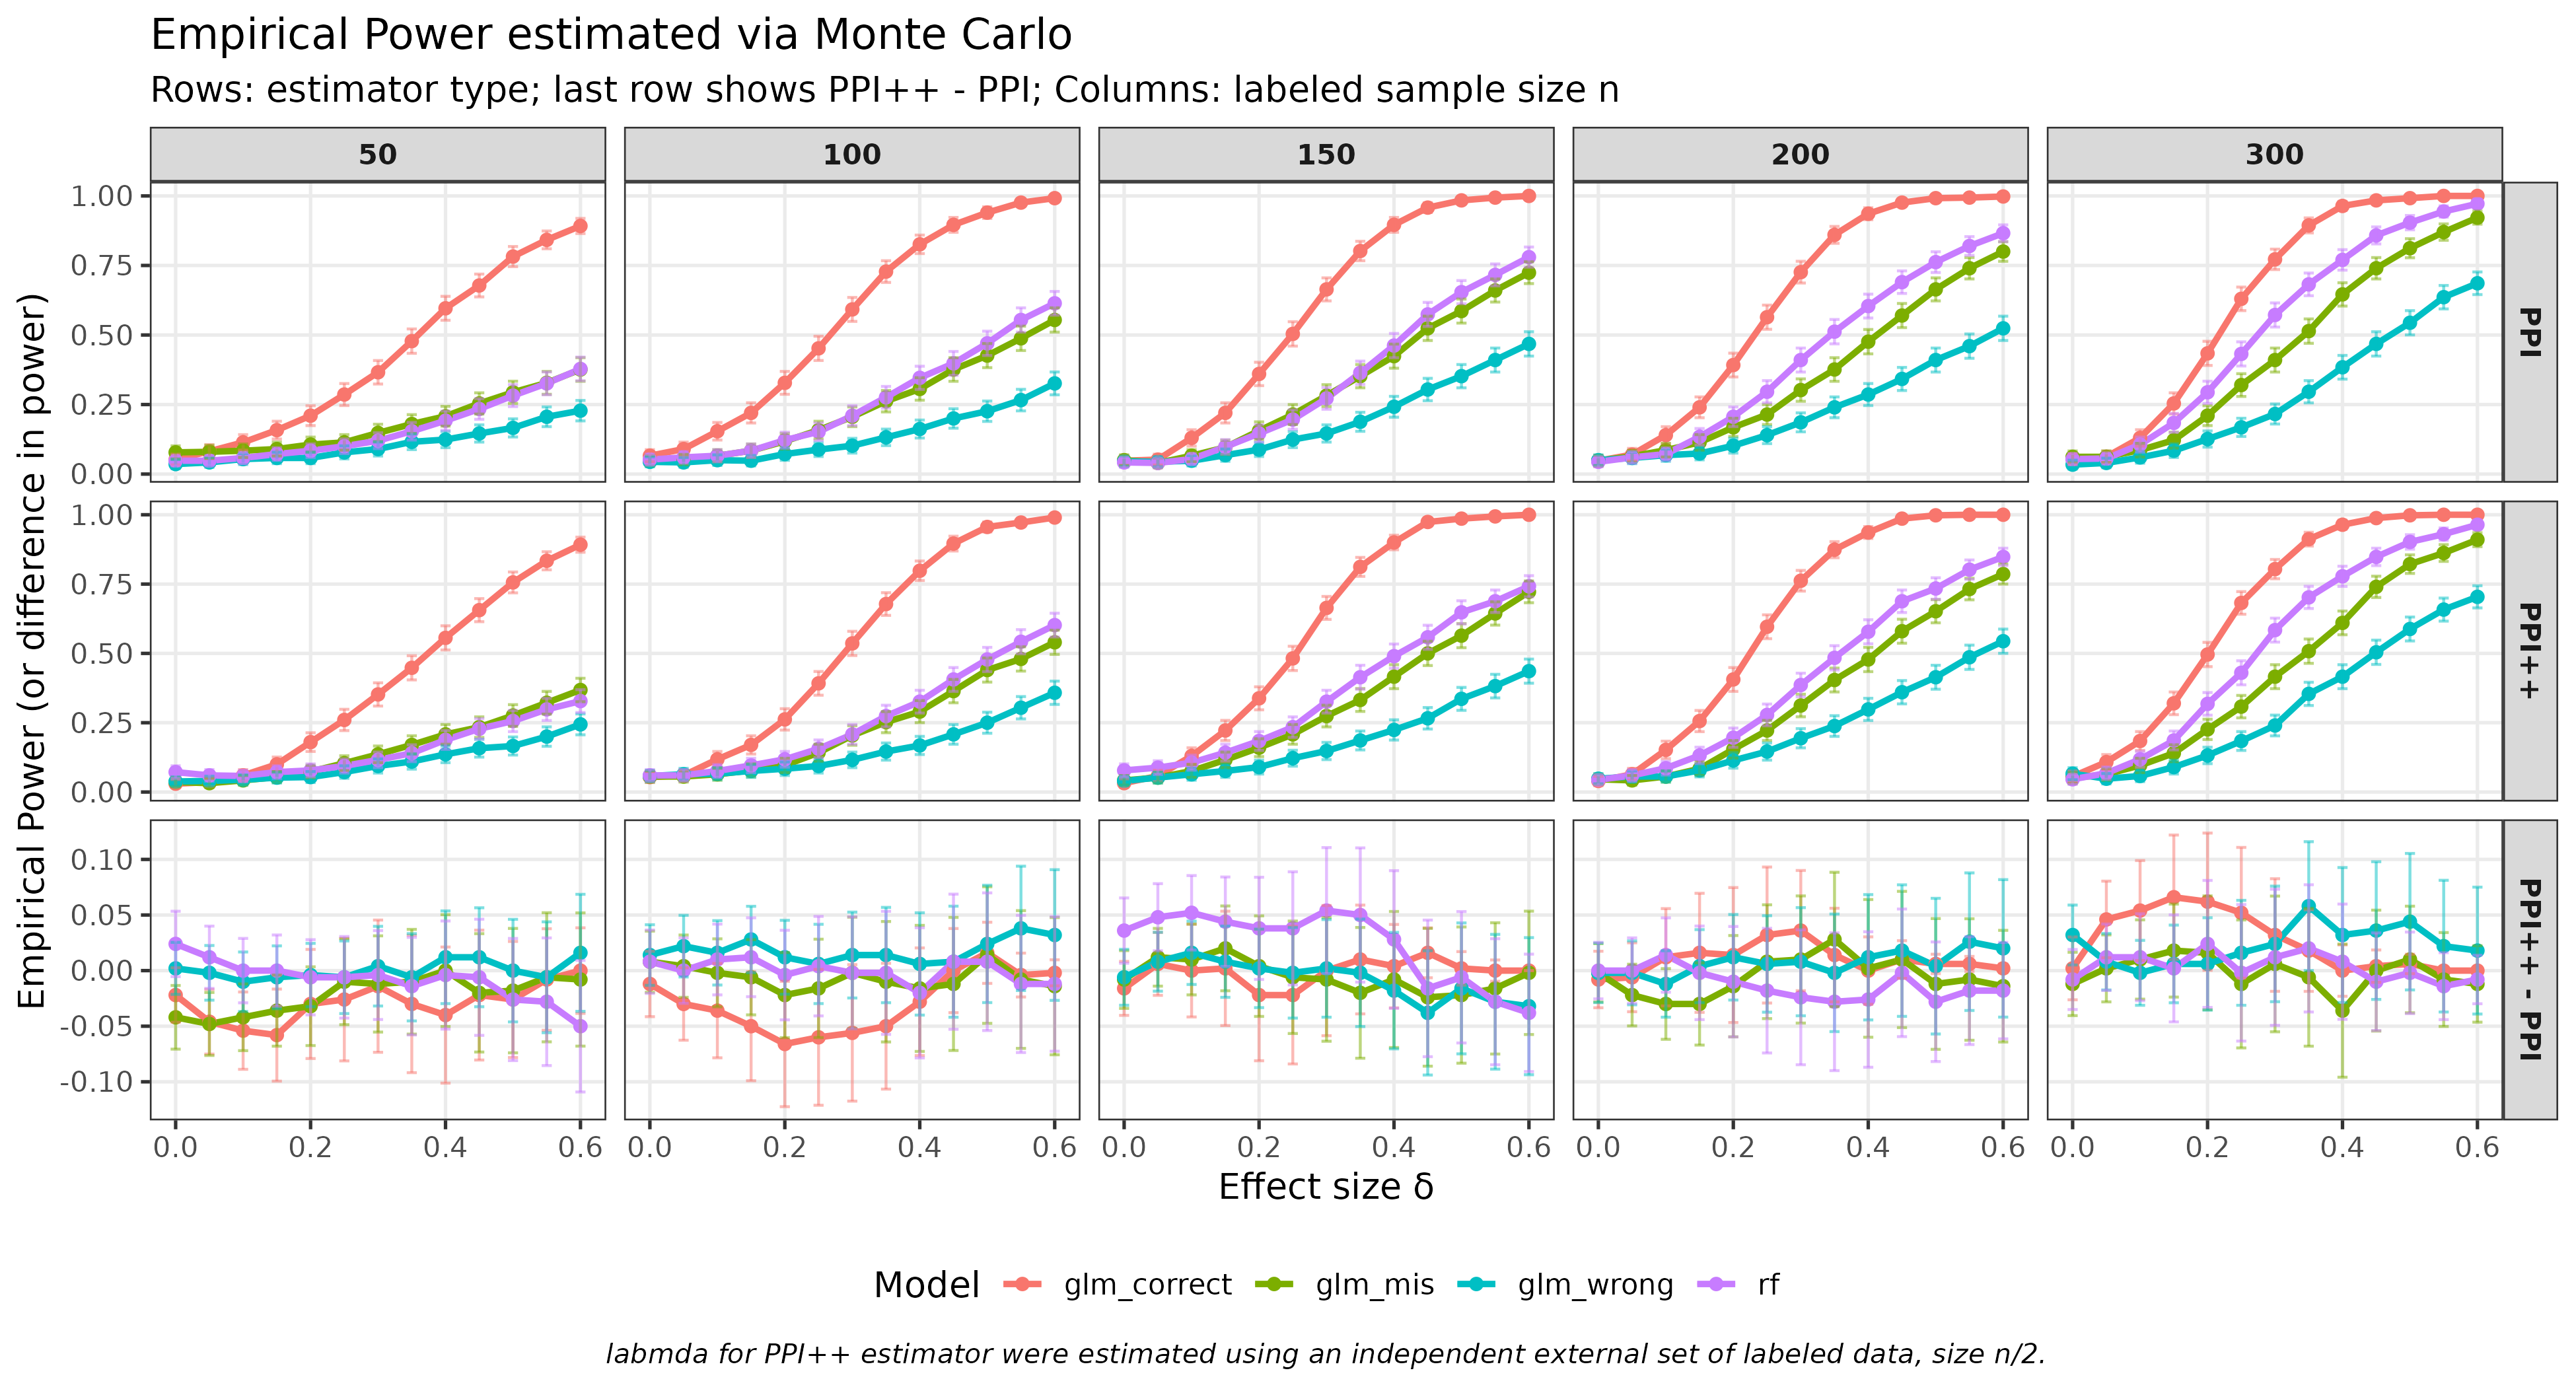
\includegraphics[width=0.95\linewidth]{power_curve_external_lambda_sample_estimates.png}
    \caption{Empirical power by estimator and labeled size $n$. Rows: (vanilla) PPI, PPI++, Difference between PPI++ and PPI.}
    \label{fig:power-by-n}
\end{figure}

\vspace{-0.5em}

\begin{figure}[!htp]
    \centering
    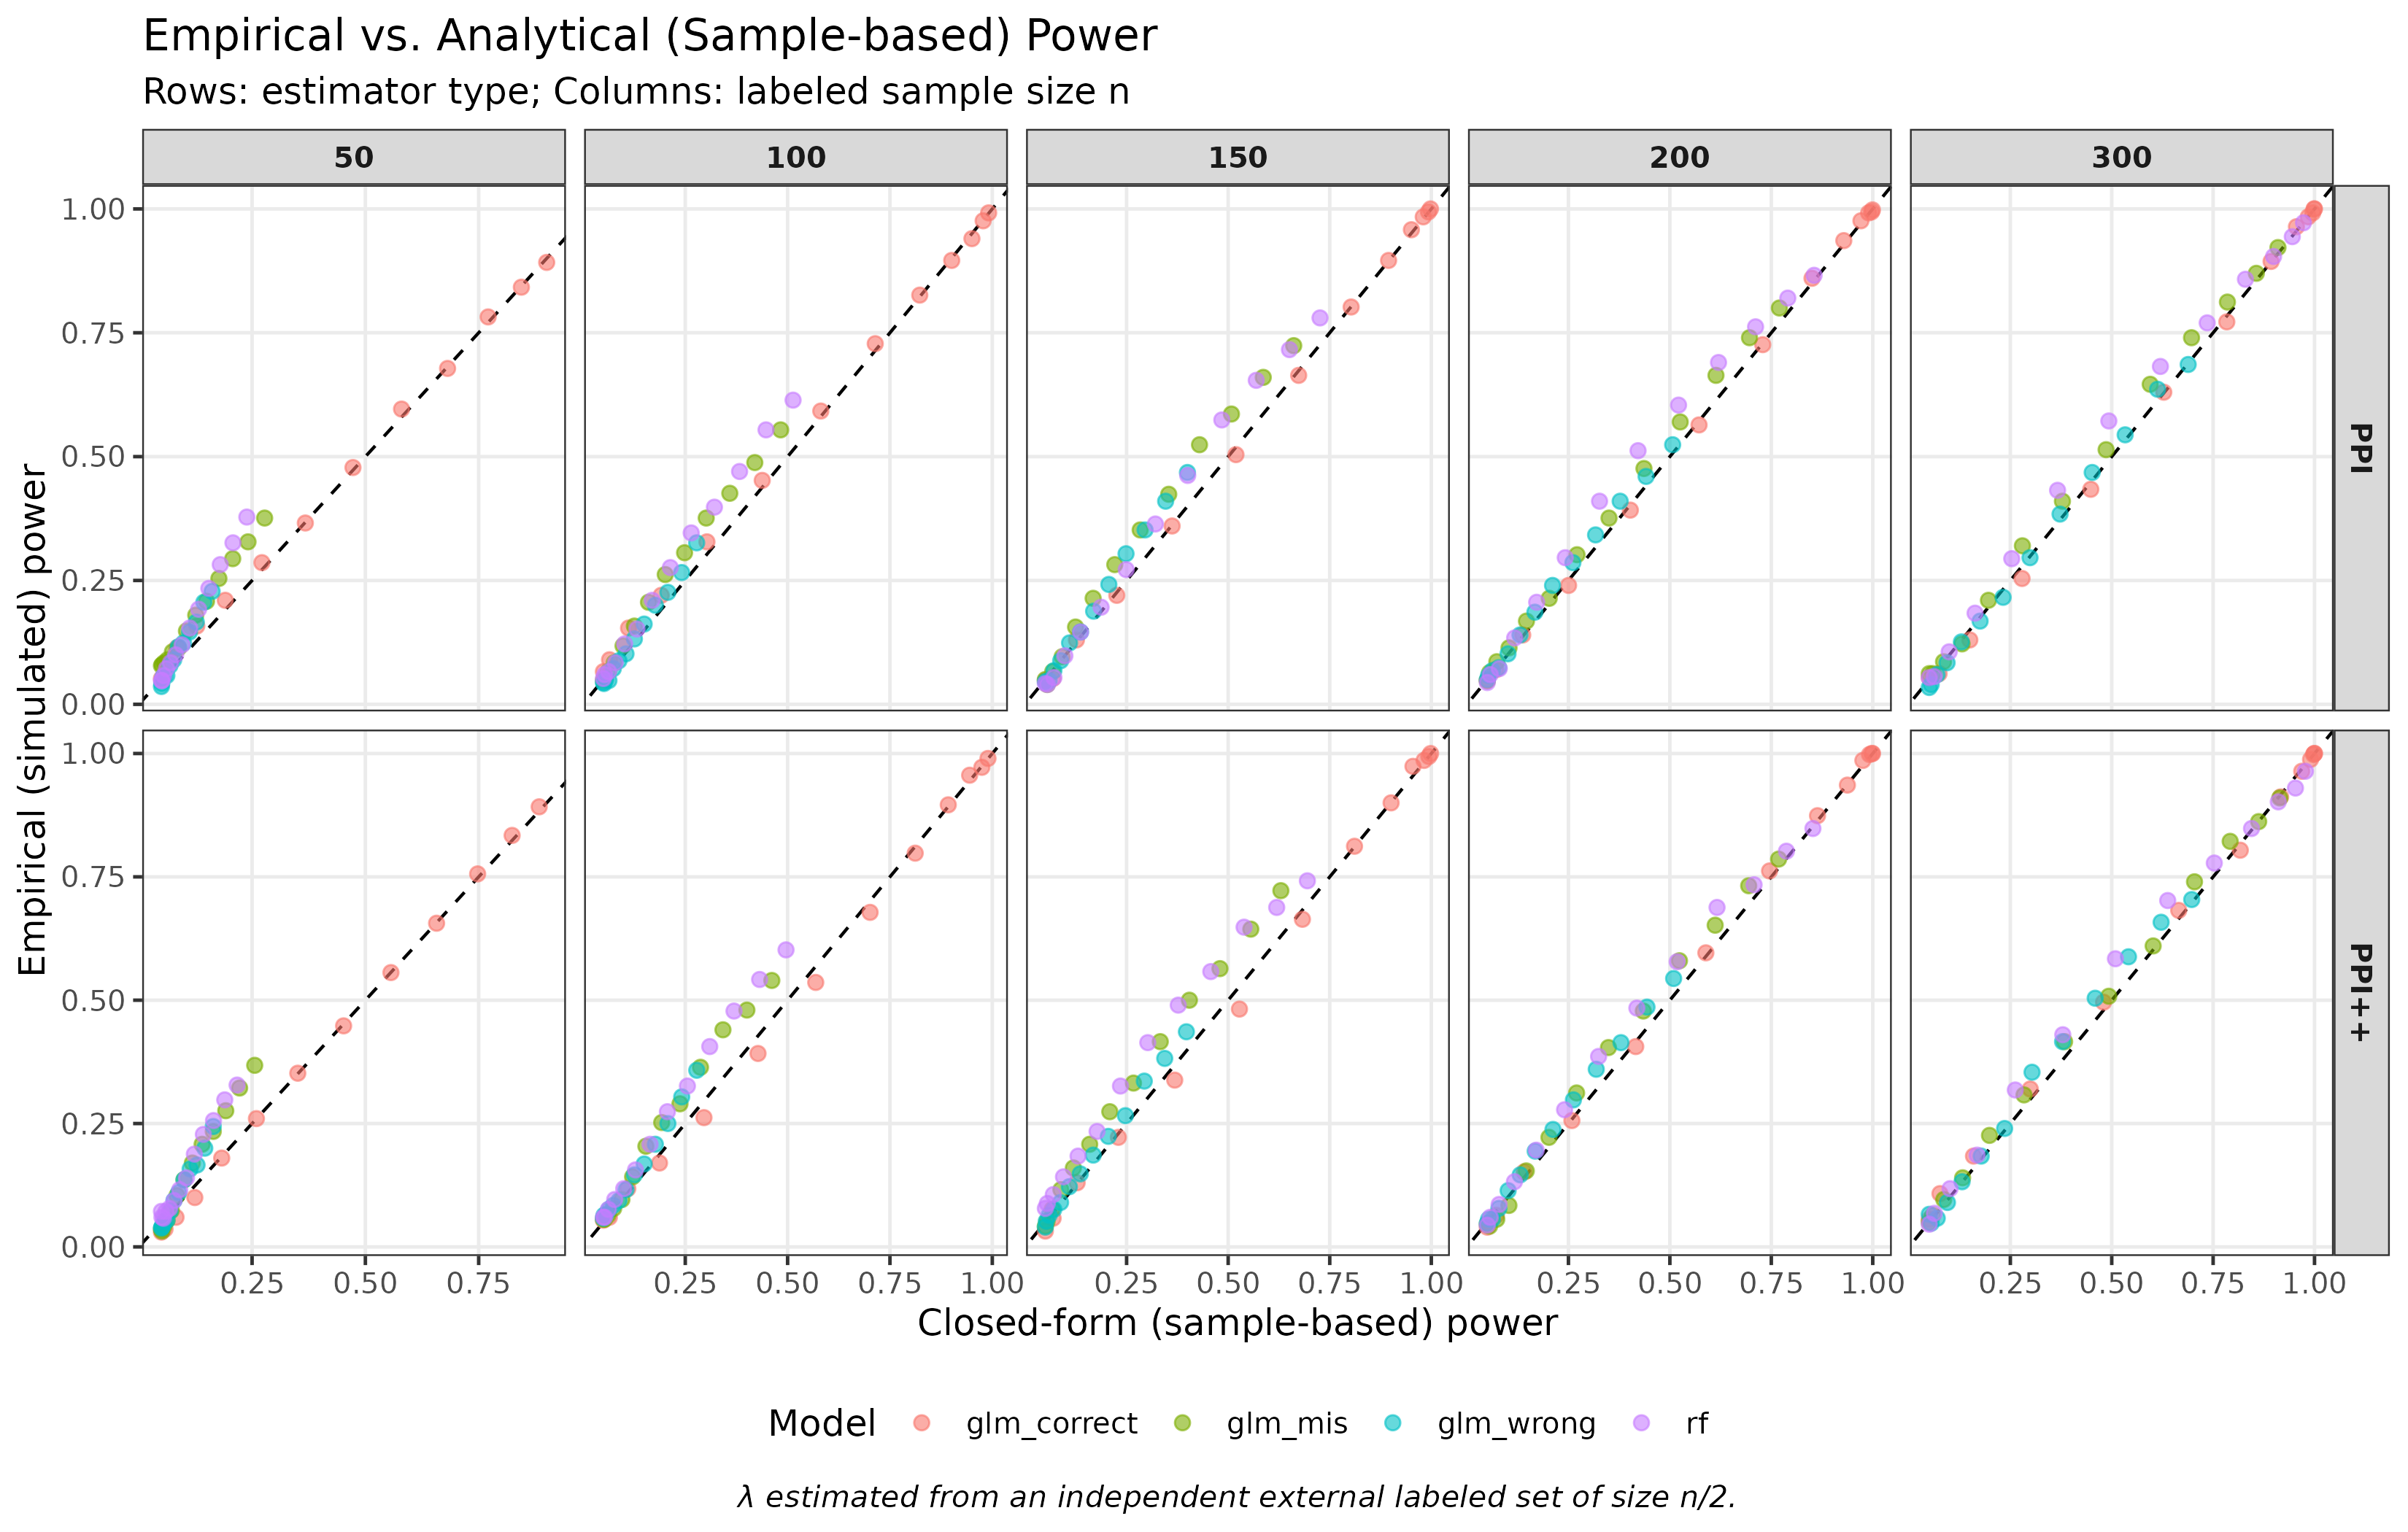
\includegraphics[width=0.95\linewidth]{analytical_empirical_power_verification_plot_sample_theoretical_power.png}
    \caption{Analytical vs. empirical power simulated by Monte Carlo. $y = x$ (dashed line) represents perfect calibration. Random forest models are not reported.}
    \label{fig:analytical-empirical-power}
\end{figure}

\begin{figure}[h!]
    \centering
    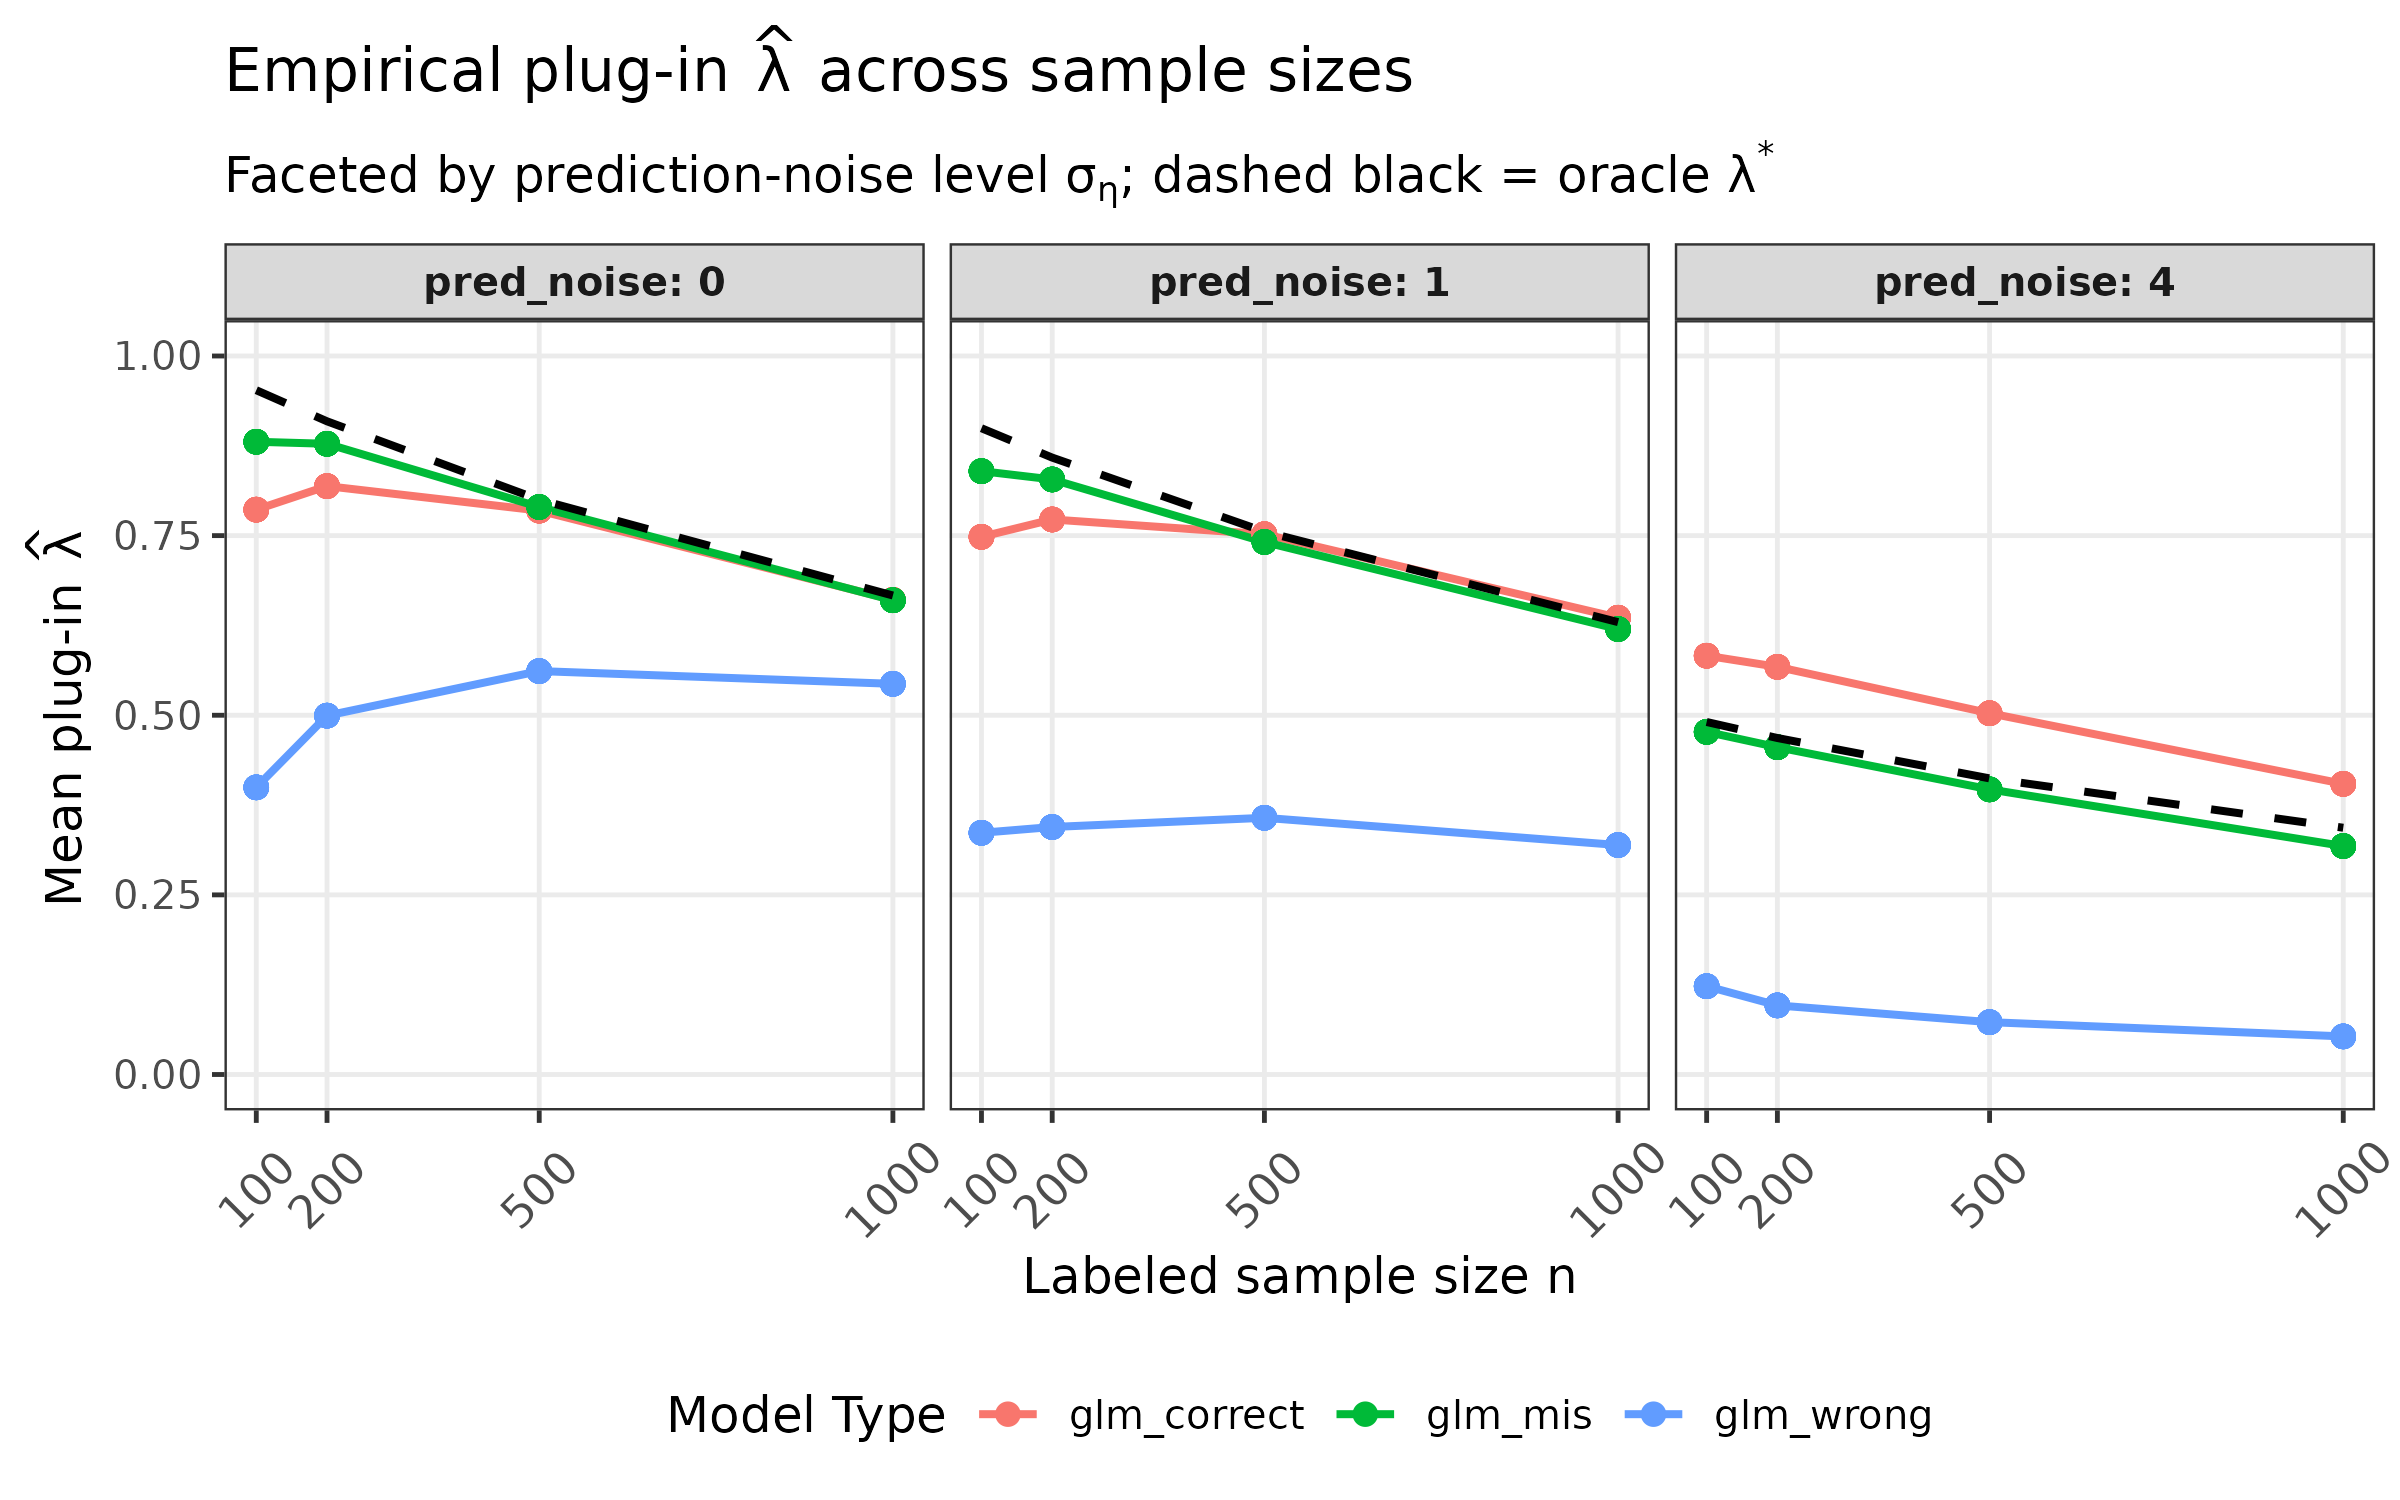
\includegraphics[width=0.99\linewidth]{lambda_empirical_vs_oracle.png}
    \caption{Empirical plug-in $\hat{\lambda}$ from PPI++ estimators across prediction noise levels $\sigma_\eta$ across different models. Oracle $\lambda^\star$ is denoted in dashed line.}
    \label{fig:pred-noise-vs-lambda}
\end{figure}

\begin{landscape}
\begin{table}
\caption{Empirical Power (Monte Carlo SE with $R = 500$) by Delta for Design = PPI\_crossfit}
\label{tab:power_delta_ppi_crossfit}

\resizebox{\linewidth}{!}{
\begin{tabular}{lllccccccccccccc}
\toprule
model\_type & ppi\_type & n & 0 & 0.05 & 0.10 & 0.15 & 0.20 & 0.25 & 0.30 & 0.35 & 0.40 & 0.45 & 0.50 & 0.550000 & 0.600000 \\
\midrule
glm\_correct & PPI & 50 & 0.036 (0.008) & 0.066 (0.011) & 0.086 (0.013) & 0.118 (0.014) & 0.162 (0.016) & 0.248 (0.019) & 0.35 (0.021) & 0.43 (0.022) & 0.55 (0.022) & 0.65 (0.021) & 0.756 (0.019) & 0.826 (0.017) & 0.878 (0.015) \\
glm\_correct & PPI & 100 & 0.036 (0.008) & 0.05 (0.01) & 0.094 (0.013) & 0.208 (0.018) & 0.316 (0.021) & 0.432 (0.022) & 0.576 (0.022) & 0.706 (0.02) & 0.83 (0.017) & 0.904 (0.013) & 0.948 (0.01) & 0.982 (0.006) & 0.996 (0.003) \\
glm\_correct & PPI & 150 & 0.042 (0.009) & 0.068 (0.011) & 0.116 (0.014) & 0.222 (0.019) & 0.35 (0.021) & 0.54 (0.022) & 0.686 (0.021) & 0.806 (0.018) & 0.892 (0.014) & 0.954 (0.009) & 0.986 (0.005) & 0.992 (0.004) & 0.994 (0.003) \\
glm\_correct & PPI & 200 & 0.064 (0.011) & 0.082 (0.012) & 0.16 (0.016) & 0.262 (0.02) & 0.402 (0.022) & 0.558 (0.022) & 0.71 (0.02) & 0.83 (0.017) & 0.902 (0.013) & 0.966 (0.008) & 0.99 (0.004) & 0.994 (0.003) & 1.0 (0.0) \\
glm\_correct & PPI & 300 & 0.034 (0.008) & 0.062 (0.011) & 0.166 (0.017) & 0.306 (0.021) & 0.476 (0.022) & 0.666 (0.021) & 0.816 (0.017) & 0.916 (0.012) & 0.976 (0.007) & 0.994 (0.003) & 0.996 (0.003) & 1.0 (0.0) & 1.0 (0.0) \\
glm\_mis & PPI & 50 & 0.032 (0.008) & 0.036 (0.008) & 0.044 (0.009) & 0.06 (0.011) & 0.094 (0.013) & 0.118 (0.014) & 0.138 (0.015) & 0.164 (0.017) & 0.216 (0.018) & 0.27 (0.02) & 0.314 (0.021) & 0.348 (0.021) & 0.394 (0.022) \\
glm\_mis & PPI & 100 & 0.038 (0.009) & 0.042 (0.009) & 0.052 (0.01) & 0.07 (0.011) & 0.106 (0.014) & 0.154 (0.016) & 0.212 (0.018) & 0.26 (0.02) & 0.314 (0.021) & 0.378 (0.022) & 0.424 (0.022) & 0.472 (0.022) & 0.532 (0.022) \\
glm\_mis & PPI & 150 & 0.042 (0.009) & 0.052 (0.01) & 0.066 (0.011) & 0.096 (0.013) & 0.124 (0.015) & 0.186 (0.017) & 0.25 (0.019) & 0.324 (0.021) & 0.412 (0.022) & 0.492 (0.022) & 0.576 (0.022) & 0.638 (0.021) & 0.694 (0.021) \\
glm\_mis & PPI & 200 & 0.078 (0.012) & 0.08 (0.012) & 0.092 (0.013) & 0.122 (0.015) & 0.162 (0.016) & 0.224 (0.019) & 0.31 (0.021) & 0.386 (0.022) & 0.472 (0.022) & 0.56 (0.022) & 0.632 (0.022) & 0.698 (0.021) & 0.754 (0.019) \\
glm\_mis & PPI & 300 & 0.038 (0.009) & 0.048 (0.01) & 0.088 (0.013) & 0.14 (0.016) & 0.208 (0.018) & 0.31 (0.021) & 0.41 (0.022) & 0.508 (0.022) & 0.634 (0.022) & 0.722 (0.02) & 0.812 (0.017) & 0.86 (0.016) & 0.902 (0.013) \\
glm\_wrong & PPI & 50 & 0.048 (0.01) & 0.044 (0.009) & 0.042 (0.009) & 0.062 (0.011) & 0.068 (0.011) & 0.068 (0.011) & 0.08 (0.012) & 0.09 (0.013) & 0.11 (0.014) & 0.13 (0.015) & 0.156 (0.016) & 0.184 (0.017) & 0.214 (0.018) \\
glm\_wrong & PPI & 100 & 0.042 (0.009) & 0.042 (0.009) & 0.046 (0.009) & 0.058 (0.01) & 0.082 (0.012) & 0.088 (0.013) & 0.108 (0.014) & 0.136 (0.015) & 0.182 (0.017) & 0.22 (0.019) & 0.28 (0.02) & 0.308 (0.021) & 0.346 (0.021) \\
glm\_wrong & PPI & 150 & 0.058 (0.01) & 0.06 (0.011) & 0.074 (0.012) & 0.082 (0.012) & 0.106 (0.014) & 0.14 (0.016) & 0.166 (0.017) & 0.206 (0.018) & 0.256 (0.02) & 0.294 (0.02) & 0.35 (0.021) & 0.414 (0.022) & 0.472 (0.022) \\
glm\_wrong & PPI & 200 & 0.04 (0.009) & 0.038 (0.009) & 0.052 (0.01) & 0.07 (0.011) & 0.104 (0.014) & 0.14 (0.016) & 0.194 (0.018) & 0.244 (0.019) & 0.302 (0.021) & 0.362 (0.021) & 0.426 (0.022) & 0.478 (0.022) & 0.544 (0.022) \\
glm\_wrong & PPI & 300 & 0.04 (0.009) & 0.036 (0.008) & 0.05 (0.01) & 0.082 (0.012) & 0.13 (0.015) & 0.2 (0.018) & 0.264 (0.02) & 0.348 (0.021) & 0.428 (0.022) & 0.506 (0.022) & 0.578 (0.022) & 0.656 (0.021) & 0.72 (0.02) \\
rf & PPI & 50 & 0.06 (0.011) & 0.064 (0.011) & 0.062 (0.011) & 0.074 (0.012) & 0.09 (0.013) & 0.114 (0.014) & 0.144 (0.016) & 0.168 (0.017) & 0.2 (0.018) & 0.242 (0.019) & 0.264 (0.02) & 0.298 (0.02) & 0.326 (0.021) \\
rf & PPI & 100 & 0.076 (0.012) & 0.084 (0.012) & 0.096 (0.013) & 0.136 (0.015) & 0.158 (0.016) & 0.18 (0.017) & 0.224 (0.019) & 0.276 (0.02) & 0.342 (0.021) & 0.396 (0.022) & 0.448 (0.022) & 0.528 (0.022) & 0.584 (0.022) \\
rf & PPI & 150 & 0.042 (0.009) & 0.05 (0.01) & 0.08 (0.012) & 0.12 (0.015) & 0.178 (0.017) & 0.246 (0.019) & 0.322 (0.021) & 0.41 (0.022) & 0.482 (0.022) & 0.572 (0.022) & 0.642 (0.021) & 0.714 (0.02) & 0.782 (0.018) \\
rf & PPI & 200 & 0.084 (0.012) & 0.088 (0.013) & 0.12 (0.015) & 0.156 (0.016) & 0.204 (0.018) & 0.3 (0.02) & 0.392 (0.022) & 0.498 (0.022) & 0.59 (0.022) & 0.676 (0.021) & 0.758 (0.019) & 0.82 (0.017) & 0.868 (0.015) \\
rf & PPI & 300 & 0.058 (0.01) & 0.068 (0.011) & 0.114 (0.014) & 0.2 (0.018) & 0.3 (0.02) & 0.422 (0.022) & 0.564 (0.022) & 0.684 (0.021) & 0.774 (0.019) & 0.858 (0.016) & 0.904 (0.013) & 0.95 (0.01) & 0.966 (0.008) \\
\bottomrule
\end{tabular}
}
\end{table}

\begin{table}
\caption{Empirical Power (Monte Carlo SE with $R = 500$) by Delta for Design = PPI\_noncrossfit}
\label{tab:power_delta_ppi_noncrossfit}
\resizebox{\linewidth}{!}{
\begin{tabular}{lllccccccccccccc}
\toprule
model\_type & ppi\_type & n & 0 & 0.05 & 0.10 & 0.15 & 0.20 & 0.25 & 0.30 & 0.35 & 0.40 & 0.45 & 0.50 & 0.55 & 0.60 \\
\midrule
glm\_correct & PPI & 50 & 0.052 (0.01) & 0.082 (0.012) & 0.114 (0.014) & 0.158 (0.016) & 0.21 (0.018) & 0.286 (0.02) & 0.366 (0.022) & 0.478 (0.022) & 0.596 (0.022) & 0.678 (0.021) & 0.782 (0.018) & 0.842 (0.016) & 0.892 (0.014) \\
glm\_correct & PPI & 100 & 0.066 (0.011) & 0.09 (0.013) & 0.154 (0.016) & 0.22 (0.019) & 0.328 (0.021) & 0.452 (0.022) & 0.592 (0.022) & 0.728 (0.02) & 0.826 (0.017) & 0.896 (0.014) & 0.94 (0.011) & 0.976 (0.007) & 0.992 (0.004) \\
glm\_correct & PPI & 150 & 0.048 (0.01) & 0.052 (0.01) & 0.13 (0.015) & 0.22 (0.019) & 0.36 (0.021) & 0.504 (0.022) & 0.664 (0.021) & 0.802 (0.018) & 0.896 (0.014) & 0.958 (0.009) & 0.984 (0.006) & 0.994 (0.003) & 1.0 (0.0) \\
glm\_correct & PPI & 200 & 0.048 (0.01) & 0.07 (0.011) & 0.14 (0.016) & 0.24 (0.019) & 0.392 (0.022) & 0.564 (0.022) & 0.726 (0.02) & 0.86 (0.016) & 0.936 (0.011) & 0.976 (0.007) & 0.992 (0.004) & 0.994 (0.003) & 0.998 (0.002) \\
glm\_correct & PPI & 300 & 0.054 (0.01) & 0.062 (0.011) & 0.13 (0.015) & 0.254 (0.019) & 0.434 (0.022) & 0.63 (0.022) & 0.772 (0.019) & 0.894 (0.014) & 0.964 (0.008) & 0.984 (0.006) & 0.992 (0.004) & 1.0 (0.0) & 1.0 (0.0) \\
glm\_mis & PPI & 50 & 0.078 (0.012) & 0.08 (0.012) & 0.084 (0.012) & 0.09 (0.013) & 0.106 (0.014) & 0.114 (0.014) & 0.148 (0.016) & 0.18 (0.017) & 0.208 (0.018) & 0.254 (0.019) & 0.294 (0.02) & 0.328 (0.021) & 0.376 (0.022) \\
glm\_mis & PPI & 100 & 0.048 (0.01) & 0.052 (0.01) & 0.066 (0.011) & 0.084 (0.012) & 0.118 (0.014) & 0.158 (0.016) & 0.206 (0.018) & 0.262 (0.02) & 0.306 (0.021) & 0.376 (0.022) & 0.426 (0.022) & 0.488 (0.022) & 0.554 (0.022) \\
glm\_mis & PPI & 150 & 0.05 (0.01) & 0.04 (0.009) & 0.066 (0.011) & 0.096 (0.013) & 0.156 (0.016) & 0.214 (0.018) & 0.282 (0.02) & 0.352 (0.021) & 0.424 (0.022) & 0.524 (0.022) & 0.586 (0.022) & 0.66 (0.021) & 0.724 (0.02) \\
glm\_mis & PPI & 200 & 0.048 (0.01) & 0.064 (0.011) & 0.086 (0.013) & 0.114 (0.014) & 0.168 (0.017) & 0.214 (0.018) & 0.302 (0.021) & 0.376 (0.022) & 0.476 (0.022) & 0.57 (0.022) & 0.664 (0.021) & 0.74 (0.02) & 0.8 (0.018) \\
glm\_mis & PPI & 300 & 0.062 (0.011) & 0.062 (0.011) & 0.086 (0.013) & 0.122 (0.015) & 0.21 (0.018) & 0.32 (0.021) & 0.41 (0.022) & 0.514 (0.022) & 0.646 (0.021) & 0.74 (0.02) & 0.812 (0.017) & 0.87 (0.015) & 0.922 (0.012) \\
glm\_wrong & PPI & 50 & 0.036 (0.008) & 0.042 (0.009) & 0.054 (0.01) & 0.058 (0.01) & 0.058 (0.01) & 0.078 (0.012) & 0.09 (0.013) & 0.116 (0.014) & 0.124 (0.015) & 0.146 (0.016) & 0.166 (0.017) & 0.206 (0.018) & 0.228 (0.019) \\
glm\_wrong & PPI & 100 & 0.044 (0.009) & 0.042 (0.009) & 0.05 (0.01) & 0.048 (0.01) & 0.072 (0.012) & 0.088 (0.013) & 0.102 (0.014) & 0.132 (0.015) & 0.162 (0.016) & 0.2 (0.018) & 0.226 (0.019) & 0.266 (0.02) & 0.326 (0.021) \\
glm\_wrong & PPI & 150 & 0.046 (0.009) & 0.044 (0.009) & 0.048 (0.01) & 0.068 (0.011) & 0.088 (0.013) & 0.124 (0.015) & 0.146 (0.016) & 0.188 (0.017) & 0.242 (0.019) & 0.304 (0.021) & 0.352 (0.021) & 0.41 (0.022) & 0.468 (0.022) \\
glm\_wrong & PPI & 200 & 0.05 (0.01) & 0.058 (0.01) & 0.068 (0.011) & 0.074 (0.012) & 0.102 (0.014) & 0.14 (0.016) & 0.186 (0.017) & 0.24 (0.019) & 0.286 (0.02) & 0.342 (0.021) & 0.41 (0.022) & 0.46 (0.022) & 0.524 (0.022) \\
glm\_wrong & PPI & 300 & 0.034 (0.008) & 0.04 (0.009) & 0.06 (0.011) & 0.084 (0.012) & 0.126 (0.015) & 0.168 (0.017) & 0.216 (0.018) & 0.296 (0.02) & 0.384 (0.022) & 0.468 (0.022) & 0.544 (0.022) & 0.636 (0.022) & 0.686 (0.021) \\
rf & PPI & 50 & 0.048 (0.01) & 0.048 (0.01) & 0.058 (0.01) & 0.072 (0.012) & 0.084 (0.012) & 0.1 (0.013) & 0.12 (0.015) & 0.154 (0.016) & 0.192 (0.018) & 0.234 (0.019) & 0.282 (0.02) & 0.326 (0.021) & 0.378 (0.022) \\
rf & PPI & 100 & 0.052 (0.01) & 0.06 (0.011) & 0.066 (0.011) & 0.084 (0.012) & 0.122 (0.015) & 0.152 (0.016) & 0.21 (0.018) & 0.276 (0.02) & 0.346 (0.021) & 0.398 (0.022) & 0.47 (0.022) & 0.554 (0.022) & 0.614 (0.022) \\
rf & PPI & 150 & 0.042 (0.009) & 0.04 (0.009) & 0.054 (0.01) & 0.098 (0.013) & 0.146 (0.016) & 0.196 (0.018) & 0.272 (0.02) & 0.364 (0.022) & 0.462 (0.022) & 0.574 (0.022) & 0.654 (0.021) & 0.716 (0.02) & 0.78 (0.019) \\
rf & PPI & 200 & 0.044 (0.009) & 0.06 (0.011) & 0.072 (0.012) & 0.134 (0.015) & 0.206 (0.018) & 0.296 (0.02) & 0.41 (0.022) & 0.512 (0.022) & 0.604 (0.022) & 0.69 (0.021) & 0.762 (0.019) & 0.82 (0.017) & 0.866 (0.015) \\
rf & PPI & 300 & 0.054 (0.01) & 0.056 (0.01) & 0.106 (0.014) & 0.184 (0.017) & 0.294 (0.02) & 0.432 (0.022) & 0.572 (0.022) & 0.682 (0.021) & 0.77 (0.019) & 0.858 (0.016) & 0.904 (0.013) & 0.944 (0.01) & 0.972 (0.007) \\
\bottomrule
\end{tabular}
}
\end{table}

\begin{table}
\caption{Empirical Power (Monte Carlo SE with $R = 500$) by Delta for Design = PPI++\_crossfit}
\label{tab:power_delta_ppi++_crossfit}
\resizebox{\linewidth}{!}{
\begin{tabular}{lllccccccccccccc}
\toprule
model\_type & ppi\_type & n & 0 & 0.05 & 0.10 & 0.15 & 0.20 & 0.25 & 0.30 & 0.35 & 0.40 & 0.45 & 0.50 & 0.55 & 0.60 \\
\midrule
glm\_correct & PPI++ & 50 & 0.05 (0.01) & 0.062 (0.011) & 0.088 (0.013) & 0.11 (0.014) & 0.136 (0.015) & 0.182 (0.017) & 0.26 (0.02) & 0.324 (0.021) & 0.428 (0.022) & 0.506 (0.022) & 0.606 (0.022) & 0.702 (0.02) & 0.748 (0.019) \\
glm\_correct & PPI++ & 100 & 0.046 (0.009) & 0.054 (0.01) & 0.094 (0.013) & 0.184 (0.017) & 0.276 (0.02) & 0.376 (0.022) & 0.488 (0.022) & 0.622 (0.022) & 0.732 (0.02) & 0.812 (0.017) & 0.888 (0.014) & 0.92 (0.012) & 0.958 (0.009) \\
glm\_correct & PPI++ & 150 & 0.05 (0.01) & 0.064 (0.011) & 0.112 (0.014) & 0.2 (0.018) & 0.306 (0.021) & 0.464 (0.022) & 0.62 (0.022) & 0.714 (0.02) & 0.834 (0.017) & 0.906 (0.013) & 0.944 (0.01) & 0.966 (0.008) & 0.984 (0.006) \\
glm\_correct & PPI++ & 200 & 0.058 (0.01) & 0.08 (0.012) & 0.138 (0.015) & 0.278 (0.02) & 0.392 (0.022) & 0.52 (0.022) & 0.676 (0.021) & 0.794 (0.018) & 0.884 (0.014) & 0.954 (0.009) & 0.986 (0.005) & 0.992 (0.004) & 1.0 (0.0) \\
glm\_correct & PPI++ & 300 & 0.034 (0.008) & 0.074 (0.012) & 0.158 (0.016) & 0.294 (0.02) & 0.488 (0.022) & 0.642 (0.021) & 0.816 (0.017) & 0.94 (0.011) & 0.976 (0.007) & 0.992 (0.004) & 0.996 (0.003) & 0.998 (0.002) & 1.0 (0.0) \\
glm\_mis & PPI++ & 50 & 0.036 (0.008) & 0.04 (0.009) & 0.044 (0.009) & 0.064 (0.011) & 0.088 (0.013) & 0.112 (0.014) & 0.134 (0.015) & 0.182 (0.017) & 0.224 (0.019) & 0.264 (0.02) & 0.306 (0.021) & 0.356 (0.021) & 0.41 (0.022) \\
glm\_mis & PPI++ & 100 & 0.038 (0.009) & 0.036 (0.008) & 0.052 (0.01) & 0.074 (0.012) & 0.114 (0.014) & 0.158 (0.016) & 0.206 (0.018) & 0.26 (0.02) & 0.306 (0.021) & 0.37 (0.022) & 0.43 (0.022) & 0.48 (0.022) & 0.542 (0.022) \\
glm\_mis & PPI++ & 150 & 0.044 (0.009) & 0.054 (0.01) & 0.076 (0.012) & 0.088 (0.013) & 0.126 (0.015) & 0.196 (0.018) & 0.254 (0.019) & 0.334 (0.021) & 0.408 (0.022) & 0.498 (0.022) & 0.568 (0.022) & 0.636 (0.022) & 0.694 (0.021) \\
glm\_mis & PPI++ & 200 & 0.07 (0.011) & 0.076 (0.012) & 0.092 (0.013) & 0.122 (0.015) & 0.162 (0.016) & 0.226 (0.019) & 0.324 (0.021) & 0.392 (0.022) & 0.476 (0.022) & 0.564 (0.022) & 0.624 (0.022) & 0.682 (0.021) & 0.758 (0.019) \\
glm\_mis & PPI++ & 300 & 0.036 (0.008) & 0.046 (0.009) & 0.076 (0.012) & 0.148 (0.016) & 0.206 (0.018) & 0.31 (0.021) & 0.42 (0.022) & 0.534 (0.022) & 0.648 (0.021) & 0.744 (0.02) & 0.824 (0.017) & 0.864 (0.015) & 0.914 (0.013) \\
glm\_wrong & PPI++ & 50 & 0.046 (0.009) & 0.046 (0.009) & 0.05 (0.01) & 0.064 (0.011) & 0.074 (0.012) & 0.078 (0.012) & 0.094 (0.013) & 0.122 (0.015) & 0.136 (0.015) & 0.154 (0.016) & 0.19 (0.018) & 0.23 (0.019) & 0.258 (0.02) \\
glm\_wrong & PPI++ & 100 & 0.046 (0.009) & 0.044 (0.009) & 0.054 (0.01) & 0.056 (0.01) & 0.082 (0.012) & 0.1 (0.013) & 0.122 (0.015) & 0.16 (0.016) & 0.21 (0.018) & 0.25 (0.019) & 0.296 (0.02) & 0.34 (0.021) & 0.376 (0.022) \\
glm\_wrong & PPI++ & 150 & 0.058 (0.01) & 0.066 (0.011) & 0.07 (0.011) & 0.09 (0.013) & 0.12 (0.015) & 0.146 (0.016) & 0.176 (0.017) & 0.21 (0.018) & 0.256 (0.02) & 0.302 (0.021) & 0.352 (0.021) & 0.418 (0.022) & 0.484 (0.022) \\
glm\_wrong & PPI++ & 200 & 0.036 (0.008) & 0.034 (0.008) & 0.056 (0.01) & 0.076 (0.012) & 0.1 (0.013) & 0.152 (0.016) & 0.212 (0.018) & 0.262 (0.02) & 0.326 (0.021) & 0.374 (0.022) & 0.442 (0.022) & 0.498 (0.022) & 0.558 (0.022) \\
glm\_wrong & PPI++ & 300 & 0.046 (0.009) & 0.038 (0.009) & 0.048 (0.01) & 0.084 (0.012) & 0.136 (0.015) & 0.186 (0.017) & 0.278 (0.02) & 0.36 (0.021) & 0.438 (0.022) & 0.516 (0.022) & 0.592 (0.022) & 0.664 (0.021) & 0.746 (0.019) \\
rf & PPI++ & 50 & 0.06 (0.011) & 0.064 (0.011) & 0.06 (0.011) & 0.07 (0.011) & 0.088 (0.013) & 0.114 (0.014) & 0.142 (0.016) & 0.164 (0.017) & 0.194 (0.018) & 0.236 (0.019) & 0.26 (0.02) & 0.296 (0.02) & 0.328 (0.021) \\
rf & PPI++ & 100 & 0.076 (0.012) & 0.082 (0.012) & 0.096 (0.013) & 0.136 (0.015) & 0.158 (0.016) & 0.178 (0.017) & 0.226 (0.019) & 0.276 (0.02) & 0.342 (0.021) & 0.396 (0.022) & 0.446 (0.022) & 0.53 (0.022) & 0.586 (0.022) \\
rf & PPI++ & 150 & 0.042 (0.009) & 0.05 (0.01) & 0.082 (0.012) & 0.118 (0.014) & 0.182 (0.017) & 0.248 (0.019) & 0.322 (0.021) & 0.41 (0.022) & 0.482 (0.022) & 0.566 (0.022) & 0.642 (0.021) & 0.714 (0.02) & 0.778 (0.019) \\
rf & PPI++ & 200 & 0.084 (0.012) & 0.088 (0.013) & 0.12 (0.015) & 0.156 (0.016) & 0.202 (0.018) & 0.298 (0.02) & 0.392 (0.022) & 0.494 (0.022) & 0.59 (0.022) & 0.676 (0.021) & 0.758 (0.019) & 0.82 (0.017) & 0.87 (0.015) \\
rf & PPI++ & 300 & 0.058 (0.01) & 0.068 (0.011) & 0.114 (0.014) & 0.198 (0.018) & 0.296 (0.02) & 0.422 (0.022) & 0.562 (0.022) & 0.684 (0.021) & 0.774 (0.019) & 0.858 (0.016) & 0.902 (0.013) & 0.95 (0.01) & 0.966 (0.008) \\
\bottomrule
\end{tabular}
}
\end{table}

\begin{table}
\caption{Empirical Power (Monte Carlo SE with $R = 500$) by Delta for Design = PPI++\_independent\_split}
\label{tab:power_delta_ppi++_independent_split}
\resizebox{\linewidth}{!}{
\begin{tabular}{lllccccccccccccc}
\toprule
model\_type & ppi\_type & n & 0.00 & 0.05 & 0.10 & 0.15 & 0.20 & 0.25 & 0.30 & 0.35 & 0.40 & 0.45 & 0.50 & 0.55 & 0.60 \\
\midrule
glm\_correct & PPI++ & 50 & 0.052 (0.01) & 0.064 (0.011) & 0.082 (0.012) & 0.124 (0.015) & 0.164 (0.017) & 0.224 (0.019) & 0.282 (0.02) & 0.372 (0.022) & 0.448 (0.022) & 0.528 (0.022) & 0.608 (0.022) & 0.674 (0.021) & 0.752 (0.019) \\
glm\_correct & PPI++ & 100 & 0.052 (0.01) & 0.07 (0.011) & 0.124 (0.015) & 0.184 (0.017) & 0.268 (0.02) & 0.386 (0.022) & 0.538 (0.022) & 0.646 (0.021) & 0.736 (0.02) & 0.824 (0.017) & 0.872 (0.015) & 0.916 (0.012) & 0.942 (0.01) \\
glm\_correct & PPI++ & 150 & 0.044 (0.009) & 0.046 (0.009) & 0.114 (0.014) & 0.212 (0.018) & 0.33 (0.021) & 0.462 (0.022) & 0.606 (0.022) & 0.728 (0.02) & 0.842 (0.016) & 0.91 (0.013) & 0.956 (0.009) & 0.98 (0.006) & 0.988 (0.005) \\
glm\_correct & PPI++ & 200 & 0.056 (0.01) & 0.068 (0.011) & 0.116 (0.014) & 0.218 (0.018) & 0.382 (0.022) & 0.542 (0.022) & 0.692 (0.021) & 0.818 (0.017) & 0.916 (0.012) & 0.954 (0.009) & 0.978 (0.007) & 0.99 (0.004) & 1.0 (0.0) \\
glm\_correct & PPI++ & 300 & 0.044 (0.009) & 0.058 (0.01) & 0.124 (0.015) & 0.264 (0.02) & 0.456 (0.022) & 0.63 (0.022) & 0.77 (0.019) & 0.888 (0.014) & 0.956 (0.009) & 0.98 (0.006) & 0.992 (0.004) & 0.998 (0.002) & 1.0 (0.0) \\
glm\_mis & PPI++ & 50 & 0.066 (0.011) & 0.07 (0.011) & 0.07 (0.011) & 0.088 (0.013) & 0.112 (0.014) & 0.126 (0.015) & 0.162 (0.016) & 0.194 (0.018) & 0.234 (0.019) & 0.284 (0.02) & 0.33 (0.021) & 0.366 (0.022) & 0.416 (0.022) \\
glm\_mis & PPI++ & 100 & 0.05 (0.01) & 0.054 (0.01) & 0.076 (0.012) & 0.09 (0.013) & 0.116 (0.014) & 0.158 (0.016) & 0.21 (0.018) & 0.282 (0.02) & 0.332 (0.021) & 0.406 (0.022) & 0.462 (0.022) & 0.518 (0.022) & 0.582 (0.022) \\
glm\_mis & PPI++ & 150 & 0.06 (0.011) & 0.048 (0.01) & 0.064 (0.011) & 0.106 (0.014) & 0.164 (0.017) & 0.23 (0.019) & 0.294 (0.02) & 0.362 (0.021) & 0.446 (0.022) & 0.554 (0.022) & 0.61 (0.022) & 0.68 (0.021) & 0.732 (0.02) \\
glm\_mis & PPI++ & 200 & 0.052 (0.01) & 0.058 (0.01) & 0.072 (0.012) & 0.114 (0.014) & 0.172 (0.017) & 0.246 (0.019) & 0.318 (0.021) & 0.412 (0.022) & 0.5 (0.022) & 0.596 (0.022) & 0.662 (0.021) & 0.76 (0.019) & 0.814 (0.017) \\
glm\_mis & PPI++ & 300 & 0.052 (0.01) & 0.062 (0.011) & 0.094 (0.013) & 0.126 (0.015) & 0.222 (0.019) & 0.34 (0.021) & 0.444 (0.022) & 0.542 (0.022) & 0.668 (0.021) & 0.75 (0.019) & 0.836 (0.017) & 0.878 (0.015) & 0.93 (0.011) \\
glm\_wrong & PPI++ & 50 & 0.042 (0.009) & 0.044 (0.009) & 0.058 (0.01) & 0.058 (0.01) & 0.056 (0.01) & 0.068 (0.011) & 0.078 (0.012) & 0.102 (0.014) & 0.124 (0.015) & 0.16 (0.016) & 0.188 (0.017) & 0.232 (0.019) & 0.256 (0.02) \\
glm\_wrong & PPI++ & 100 & 0.048 (0.01) & 0.034 (0.008) & 0.046 (0.009) & 0.046 (0.009) & 0.066 (0.011) & 0.086 (0.013) & 0.106 (0.014) & 0.152 (0.016) & 0.188 (0.017) & 0.222 (0.019) & 0.258 (0.02) & 0.294 (0.02) & 0.344 (0.021) \\
glm\_wrong & PPI++ & 150 & 0.048 (0.01) & 0.04 (0.009) & 0.046 (0.009) & 0.08 (0.012) & 0.096 (0.013) & 0.132 (0.015) & 0.164 (0.017) & 0.206 (0.018) & 0.258 (0.02) & 0.32 (0.021) & 0.37 (0.022) & 0.43 (0.022) & 0.494 (0.022) \\
glm\_wrong & PPI++ & 200 & 0.044 (0.009) & 0.054 (0.01) & 0.064 (0.011) & 0.074 (0.012) & 0.108 (0.014) & 0.148 (0.016) & 0.19 (0.018) & 0.246 (0.019) & 0.296 (0.02) & 0.362 (0.021) & 0.43 (0.022) & 0.474 (0.022) & 0.538 (0.022) \\
glm\_wrong & PPI++ & 300 & 0.042 (0.009) & 0.046 (0.009) & 0.062 (0.011) & 0.092 (0.013) & 0.124 (0.015) & 0.174 (0.017) & 0.248 (0.019) & 0.316 (0.021) & 0.404 (0.022) & 0.504 (0.022) & 0.57 (0.022) & 0.652 (0.021) & 0.708 (0.02) \\
rf & PPI++ & 50 & 0.05 (0.01) & 0.052 (0.01) & 0.062 (0.011) & 0.08 (0.012) & 0.088 (0.013) & 0.098 (0.013) & 0.114 (0.014) & 0.16 (0.016) & 0.2 (0.018) & 0.242 (0.019) & 0.276 (0.02) & 0.316 (0.021) & 0.366 (0.022) \\
rf & PPI++ & 100 & 0.054 (0.01) & 0.058 (0.01) & 0.066 (0.011) & 0.084 (0.012) & 0.122 (0.015) & 0.156 (0.016) & 0.21 (0.018) & 0.274 (0.02) & 0.344 (0.021) & 0.398 (0.022) & 0.472 (0.022) & 0.558 (0.022) & 0.61 (0.022) \\
rf & PPI++ & 150 & 0.042 (0.009) & 0.038 (0.009) & 0.058 (0.01) & 0.096 (0.013) & 0.142 (0.016) & 0.194 (0.018) & 0.272 (0.02) & 0.364 (0.022) & 0.458 (0.022) & 0.574 (0.022) & 0.648 (0.021) & 0.71 (0.02) & 0.778 (0.019) \\
rf & PPI++ & 200 & 0.04 (0.009) & 0.058 (0.01) & 0.074 (0.012) & 0.138 (0.015) & 0.204 (0.018) & 0.288 (0.02) & 0.402 (0.022) & 0.506 (0.022) & 0.6 (0.022) & 0.684 (0.021) & 0.762 (0.019) & 0.816 (0.017) & 0.868 (0.015) \\
rf & PPI++ & 300 & 0.052 (0.01) & 0.058 (0.01) & 0.1 (0.013) & 0.184 (0.017) & 0.296 (0.02) & 0.43 (0.022) & 0.568 (0.022) & 0.686 (0.021) & 0.766 (0.019) & 0.856 (0.016) & 0.904 (0.013) & 0.944 (0.01) & 0.972 (0.007) \\
\bottomrule
\end{tabular}
}
\end{table}

\begin{table}
\caption{Empirical Power (Monte Carlo SE with $R = 500$) by Delta for Design = PPI++\_noncrossfit}
\label{tab:power_delta_ppi++_noncrossfit}
\resizebox{\linewidth}{!}{
\begin{tabular}{lllccccccccccccc}
\toprule
model\_type & ppi\_type & n & 0.00 & 0.05 & 0.10 & 0.15 & 0.20 & 0.25 & 0.30 & 0.35 & 0.40 & 0.45 & 0.50 & 0.55 & 0.60 \\
\midrule
glm\_correct & PPI++ & 50 & 0.056 (0.01) & 0.068 (0.011) & 0.098 (0.013) & 0.14 (0.016) & 0.188 (0.017) & 0.244 (0.019) & 0.32 (0.021) & 0.402 (0.022) & 0.494 (0.022) & 0.57 (0.022) & 0.658 (0.021) & 0.734 (0.02) & 0.784 (0.018) \\
glm\_correct & PPI++ & 100 & 0.048 (0.01) & 0.056 (0.01) & 0.112 (0.014) & 0.184 (0.017) & 0.284 (0.02) & 0.39 (0.022) & 0.524 (0.022) & 0.626 (0.022) & 0.728 (0.02) & 0.816 (0.017) & 0.89 (0.014) & 0.936 (0.011) & 0.962 (0.009) \\
glm\_correct & PPI++ & 150 & 0.058 (0.01) & 0.086 (0.013) & 0.122 (0.015) & 0.21 (0.018) & 0.348 (0.021) & 0.468 (0.022) & 0.608 (0.022) & 0.762 (0.019) & 0.848 (0.016) & 0.906 (0.013) & 0.948 (0.01) & 0.974 (0.007) & 0.986 (0.005) \\
glm\_correct & PPI++ & 200 & 0.048 (0.01) & 0.048 (0.01) & 0.13 (0.015) & 0.226 (0.019) & 0.382 (0.022) & 0.544 (0.022) & 0.682 (0.021) & 0.806 (0.018) & 0.9 (0.013) & 0.948 (0.01) & 0.97 (0.008) & 0.99 (0.004) & 0.998 (0.002) \\
glm\_correct & PPI++ & 300 & 0.058 (0.01) & 0.072 (0.012) & 0.144 (0.016) & 0.308 (0.021) & 0.462 (0.022) & 0.666 (0.021) & 0.812 (0.017) & 0.896 (0.014) & 0.956 (0.009) & 0.986 (0.005) & 0.994 (0.003) & 0.996 (0.003) & 1.0 (0.0) \\
glm\_mis & PPI++ & 50 & 0.048 (0.01) & 0.052 (0.01) & 0.058 (0.01) & 0.08 (0.012) & 0.11 (0.014) & 0.14 (0.016) & 0.172 (0.017) & 0.216 (0.018) & 0.232 (0.019) & 0.276 (0.02) & 0.338 (0.021) & 0.382 (0.022) & 0.43 (0.022) \\
glm\_mis & PPI++ & 100 & 0.058 (0.01) & 0.054 (0.01) & 0.084 (0.012) & 0.098 (0.013) & 0.132 (0.015) & 0.188 (0.017) & 0.24 (0.019) & 0.282 (0.02) & 0.354 (0.021) & 0.414 (0.022) & 0.496 (0.022) & 0.564 (0.022) & 0.628 (0.022) \\
glm\_mis & PPI++ & 150 & 0.06 (0.011) & 0.072 (0.012) & 0.074 (0.012) & 0.124 (0.015) & 0.176 (0.017) & 0.242 (0.019) & 0.306 (0.021) & 0.376 (0.022) & 0.436 (0.022) & 0.51 (0.022) & 0.626 (0.022) & 0.71 (0.02) & 0.762 (0.019) \\
glm\_mis & PPI++ & 200 & 0.048 (0.01) & 0.06 (0.011) & 0.076 (0.012) & 0.144 (0.016) & 0.194 (0.018) & 0.28 (0.02) & 0.368 (0.022) & 0.442 (0.022) & 0.55 (0.022) & 0.62 (0.022) & 0.696 (0.021) & 0.768 (0.019) & 0.82 (0.017) \\
glm\_mis & PPI++ & 300 & 0.038 (0.009) & 0.04 (0.009) & 0.104 (0.014) & 0.152 (0.016) & 0.234 (0.019) & 0.336 (0.021) & 0.44 (0.022) & 0.536 (0.022) & 0.632 (0.022) & 0.716 (0.02) & 0.792 (0.018) & 0.866 (0.015) & 0.898 (0.014) \\
glm\_wrong & PPI++ & 50 & 0.048 (0.01) & 0.06 (0.011) & 0.07 (0.011) & 0.08 (0.012) & 0.084 (0.012) & 0.098 (0.013) & 0.116 (0.014) & 0.142 (0.016) & 0.152 (0.016) & 0.18 (0.017) & 0.202 (0.018) & 0.224 (0.019) & 0.27 (0.02) \\
glm\_wrong & PPI++ & 100 & 0.042 (0.009) & 0.048 (0.01) & 0.058 (0.01) & 0.078 (0.012) & 0.104 (0.014) & 0.122 (0.015) & 0.158 (0.016) & 0.184 (0.017) & 0.222 (0.019) & 0.258 (0.02) & 0.296 (0.02) & 0.332 (0.021) & 0.386 (0.022) \\
glm\_wrong & PPI++ & 150 & 0.046 (0.009) & 0.06 (0.011) & 0.068 (0.011) & 0.084 (0.012) & 0.102 (0.014) & 0.142 (0.016) & 0.184 (0.017) & 0.236 (0.019) & 0.268 (0.02) & 0.32 (0.021) & 0.368 (0.022) & 0.426 (0.022) & 0.476 (0.022) \\
glm\_wrong & PPI++ & 200 & 0.06 (0.011) & 0.07 (0.011) & 0.074 (0.012) & 0.084 (0.012) & 0.11 (0.014) & 0.136 (0.015) & 0.186 (0.017) & 0.256 (0.02) & 0.326 (0.021) & 0.406 (0.022) & 0.47 (0.022) & 0.536 (0.022) & 0.602 (0.022) \\
glm\_wrong & PPI++ & 300 & 0.054 (0.01) & 0.062 (0.011) & 0.088 (0.013) & 0.124 (0.015) & 0.152 (0.016) & 0.196 (0.018) & 0.246 (0.019) & 0.32 (0.021) & 0.414 (0.022) & 0.496 (0.022) & 0.562 (0.022) & 0.63 (0.022) & 0.7 (0.02) \\
rf & PPI++ & 50 & 0.308 (0.021) & 0.322 (0.021) & 0.35 (0.021) & 0.372 (0.022) & 0.406 (0.022) & 0.444 (0.022) & 0.512 (0.022) & 0.546 (0.022) & 0.586 (0.022) & 0.642 (0.021) & 0.682 (0.021) & 0.728 (0.02) & 0.766 (0.019) \\
rf & PPI++ & 100 & 0.308 (0.021) & 0.318 (0.021) & 0.338 (0.021) & 0.38 (0.022) & 0.444 (0.022) & 0.506 (0.022) & 0.576 (0.022) & 0.684 (0.021) & 0.734 (0.02) & 0.782 (0.018) & 0.84 (0.016) & 0.88 (0.015) & 0.916 (0.012) \\
rf & PPI++ & 150 & 0.252 (0.019) & 0.268 (0.02) & 0.292 (0.02) & 0.38 (0.022) & 0.474 (0.022) & 0.57 (0.022) & 0.658 (0.021) & 0.744 (0.02) & 0.824 (0.017) & 0.882 (0.014) & 0.928 (0.012) & 0.958 (0.009) & 0.976 (0.007) \\
rf & PPI++ & 200 & 0.212 (0.018) & 0.242 (0.019) & 0.292 (0.02) & 0.384 (0.022) & 0.504 (0.022) & 0.628 (0.022) & 0.738 (0.02) & 0.824 (0.017) & 0.902 (0.013) & 0.95 (0.01) & 0.968 (0.008) & 0.986 (0.005) & 0.99 (0.004) \\
rf & PPI++ & 300 & 0.174 (0.017) & 0.21 (0.018) & 0.286 (0.02) & 0.418 (0.022) & 0.568 (0.022) & 0.738 (0.02) & 0.854 (0.016) & 0.928 (0.012) & 0.968 (0.008) & 0.992 (0.004) & 0.994 (0.003) & 0.998 (0.002) & 1.0 (0.0) \\
\bottomrule
\end{tabular}
}
\end{table}


\end{landscape}


\end{document}
